\clearpage
\appendix

\section{Trends in Identity Theft from 2008-2021}
\label{app:longitudinal}

Beyond the average characteristics over the entire study period of 2008 to 2021, examining the trends year by year reveals shifts in the type of theft, as well as how victims experience them. Figures  \ref{fig:theft_type_long} and \ref{fig:discovery_method_long}  illustrate these patterns, showing how the crime itself, the way victims discover it, and its financial impact have changed from 2008 to 2021. 

First, considering the types of identity theft experienced, Figure \ref{fig:theft_type_long} shows a shift from traditional financial account misuse to other forms, which is particularly evident in the most recent survey year, 2021. As shown, existing bank account or credit card misuse remain the most common types of identity theft experienced. Misuse of existing credit cards, historically the most prevalent type (affecting over 50\% of victims in some years), saw a substantial decline between 2018 and 2021, dropping to roughly 38\%. Existing bank account misuse followed a similar pattern, also decreasing significantly in 2021. In contrast, the category of "Other Existing Account Misuse," which includes misuse of online accounts like email or social media, experienced a dramatic surge in 2021, rising from around 10\% in 2018 to over 30\% of victims in 2021. This indicates a significant change in criminal activity towards compromising online credentials. This could also be due to the rapid rise of social media over the last few years. New account fraud and other misuses of personal information remained relatively stable at lower prevalence levels throughout the period.


\begin{figure}[htbp]
    \centering
    % --- Subfigure A: Counts ---
    \begin{subfigure}[b]{0.48\textwidth}
        \centering
        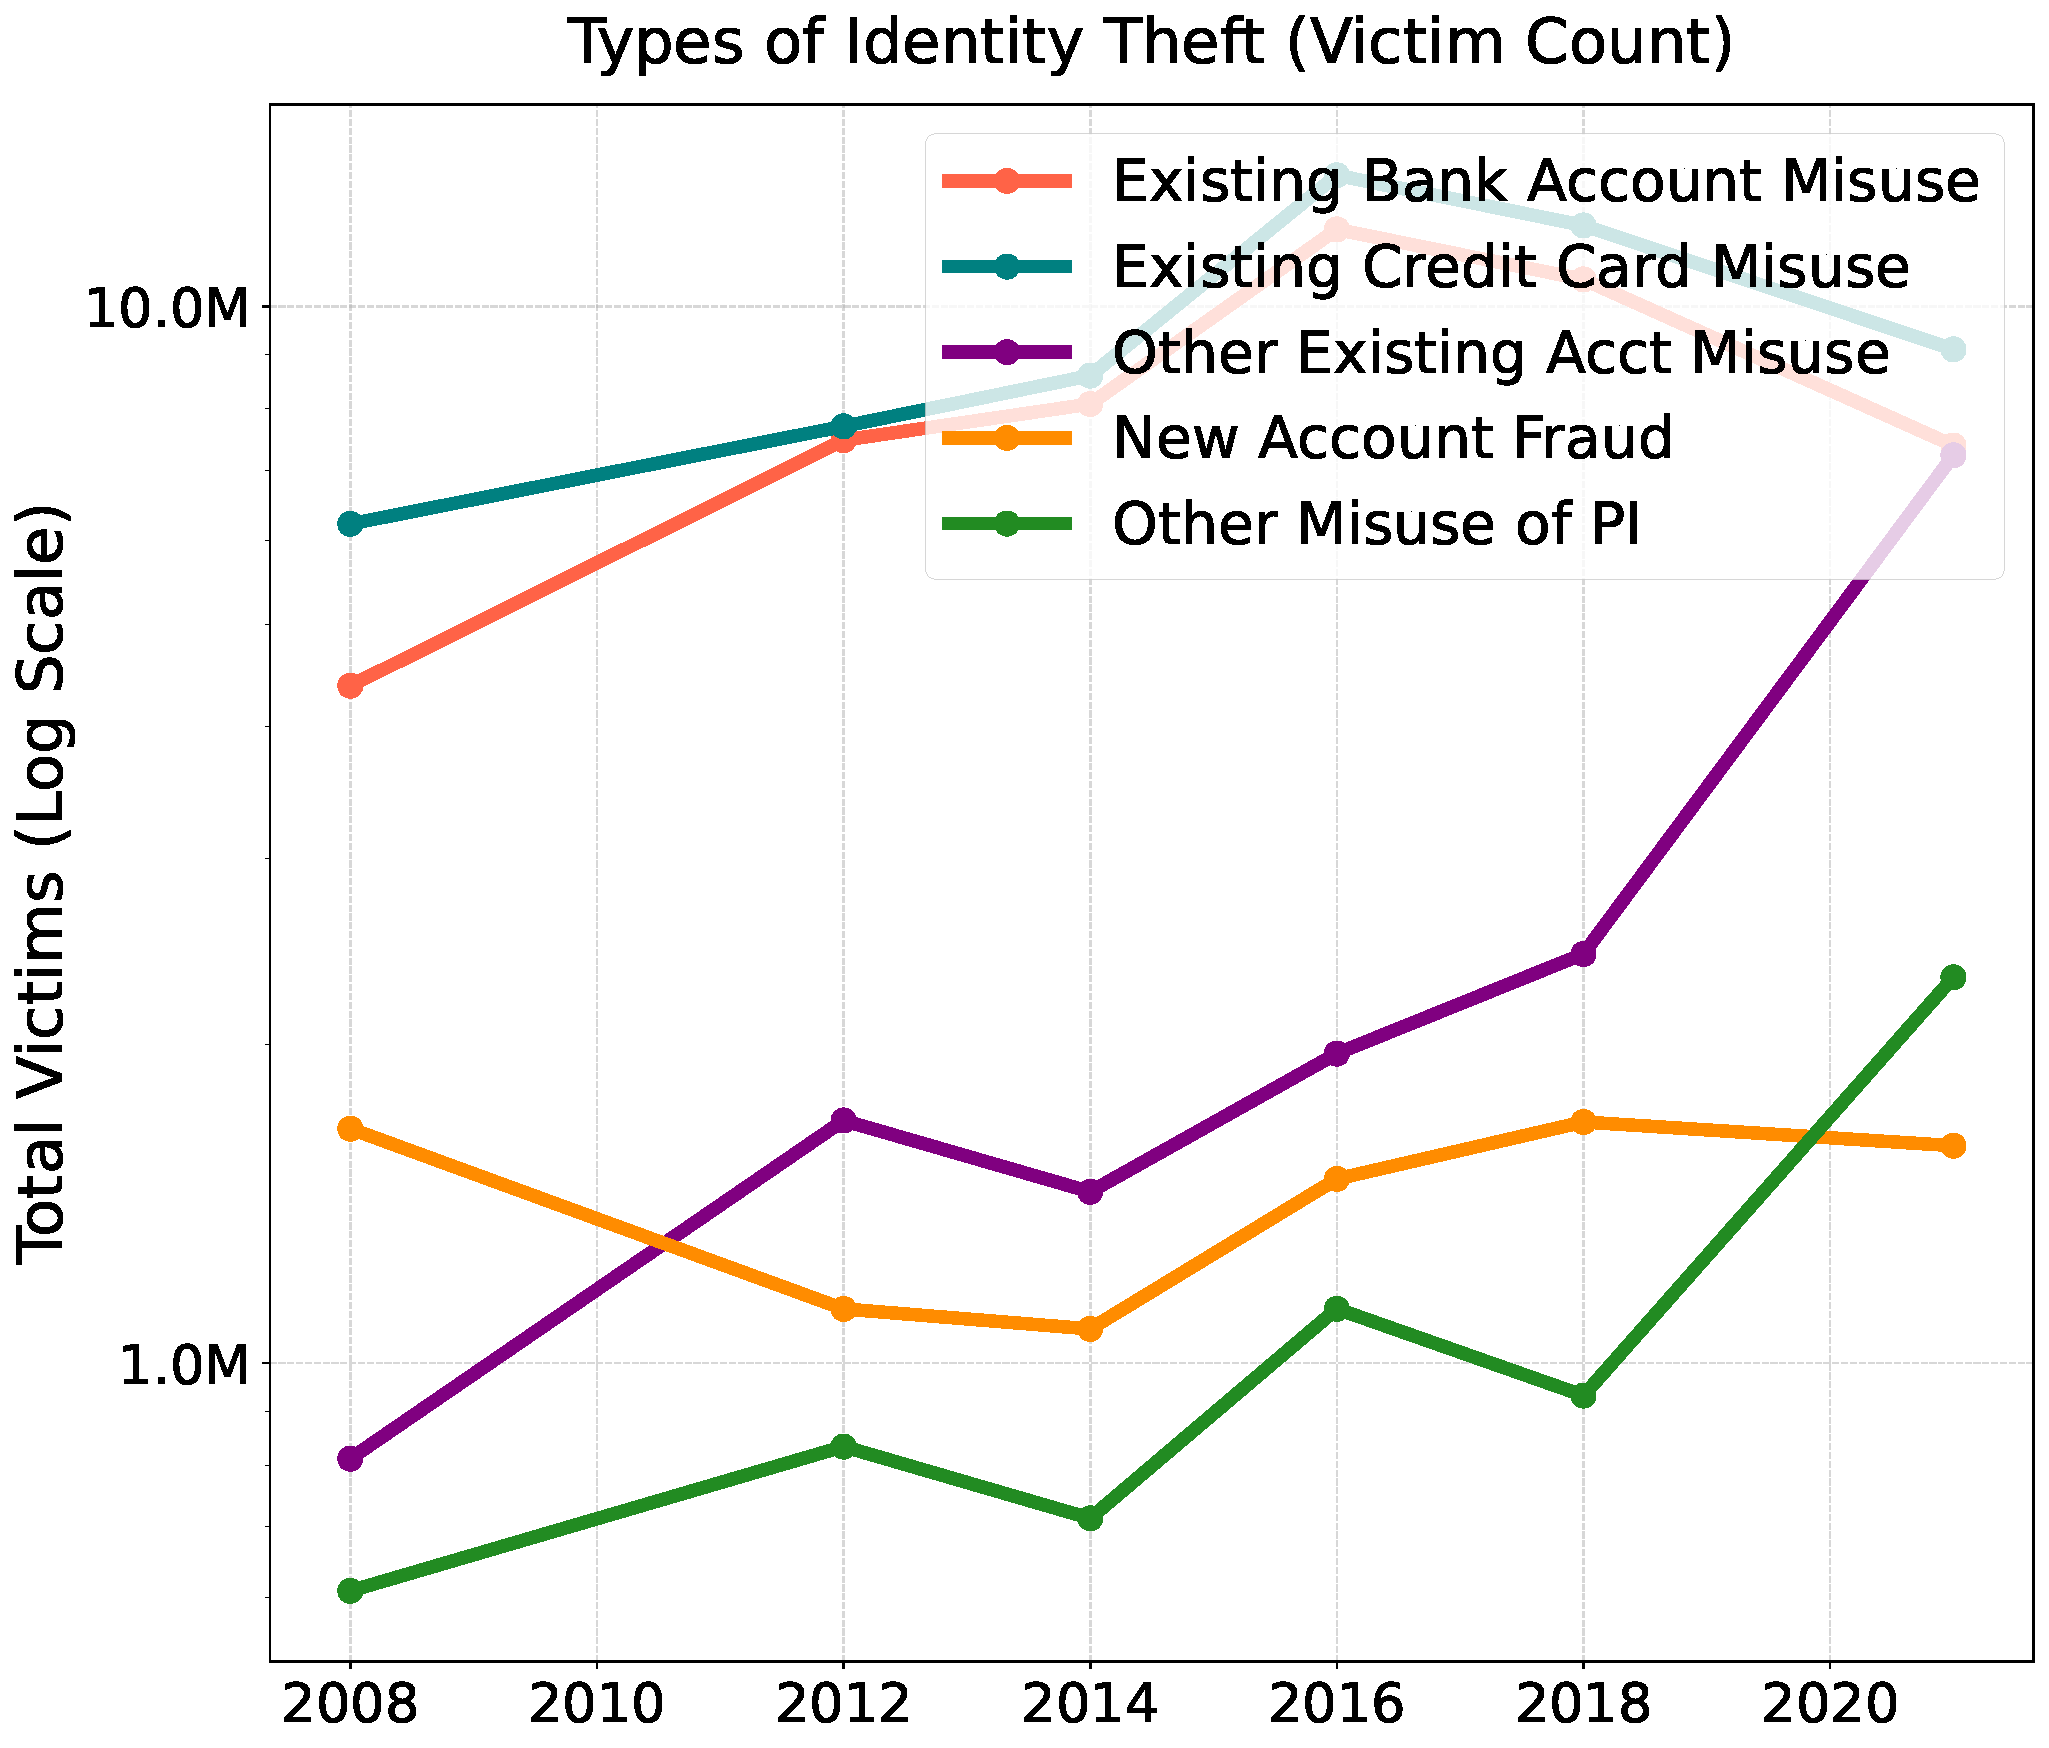
\includegraphics[width=\textwidth]{figures/incident_trends/plot2_theft_types_count.pdf}
        \caption{Number of victims categorized by the type of identity theft they suffered from.}
        \label{fig:theft_type_long_a}
    \end{subfigure}
    \hfill
    % --- Subfigure B: Percentages ---
    \begin{subfigure}[b]{0.48\textwidth}
        \centering
        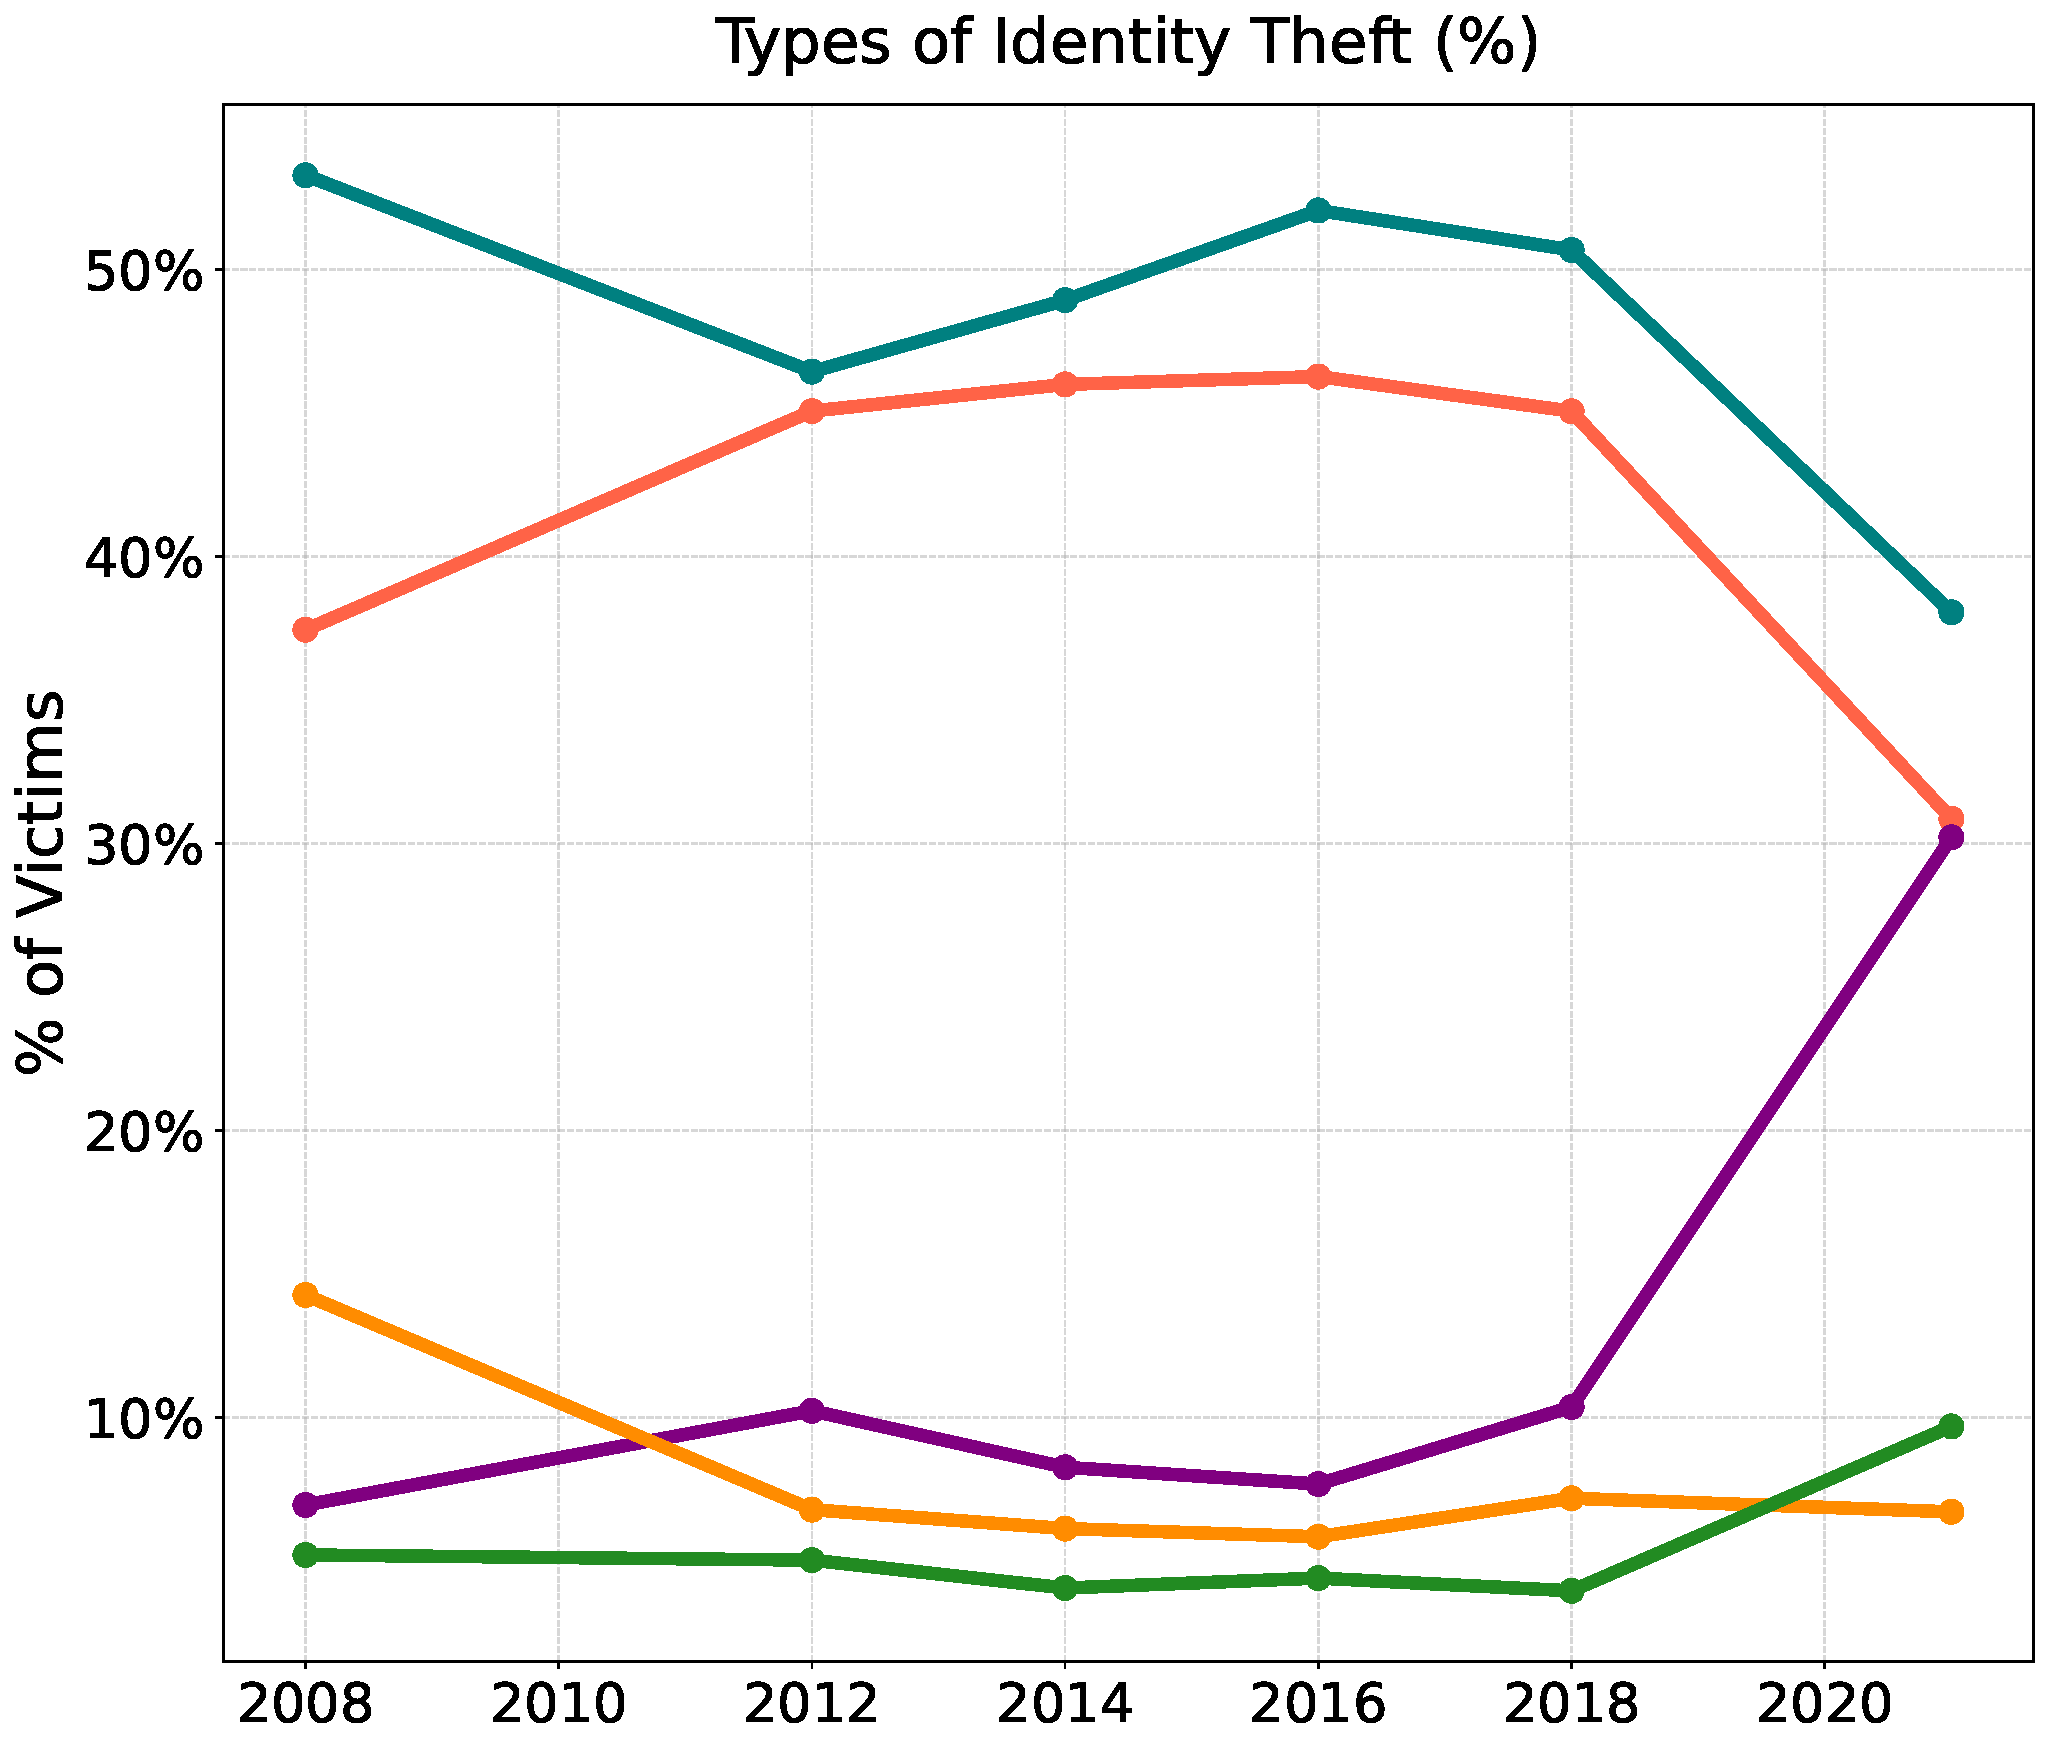
\includegraphics[width=\textwidth]{figures/incident_trends/plot2_theft_types_percentage.pdf}
        \caption{Percentage of victims categorized by the type of identity theft they suffered from.}
        \label{fig:theft_type_long_b}
    \end{subfigure}
    
    \caption{Analysis of theft types over the longitudinal study period.}
    \label{fig:theft_type_long}
\end{figure}

% Figure \ref{fig:theft_method_long} displays how victims reported their information was obtained by offenders, which adds more context to the nature of the crime they suffered. A noticeable trend is the considerable decline in information being compromised during a transaction. This method, although always the most common identified theft method, peaked in 2012 and 2014, and then fell sharply after, accounting for less than 8\% in 2021. Note that in October 2015, the major credit card networks (Europay, MasterCard, and Visa) implemented the EMV liability shift, a policy change that transferred financial responsibility for in-person counterfeit card fraud from the card issuer to whichever party in the transaction (either the merchant or the issuer) had not adopted the more secure chip card technology. This was not a government mandated law but rather a policy change by the major credit card networks to financially incentivize the adoption of chip technology. The policy forced a nationwide payment infrastructure upgrade in an effort to counter the vulnerability of the easily cloned magnetic strip, which had been a leading carrier of counterfeit card fraud. The EMV liability shift was a major turning point in the fight against in-person payment fraud. The reduction in information being stolen during a transaction in Figure \ref{fig:theft_method_long} aligns with the time frame of the October 2015 liability shift for EMV chip card adoption in the United States. The efficacy of this transition was reported by the Federal Reserve, which reported that in-person card fraud, including counterfeit cards, declined from \$3.68 billion in 2015 to \$2.91 billion in 2016 \cite{fed2018fraud}. Similarly, Visa also reported that by October 2016, counterfeit fraud dollars at chip enabled merchants had dropped by 43\% compared to a year earlier \cite{visa2016infographic}, and later data showed this decline reached 66\% by June 2017 \cite{visa2017report}.

% \begin{wrapfigure}{r}{0.5\textwidth}
%     \centering
%     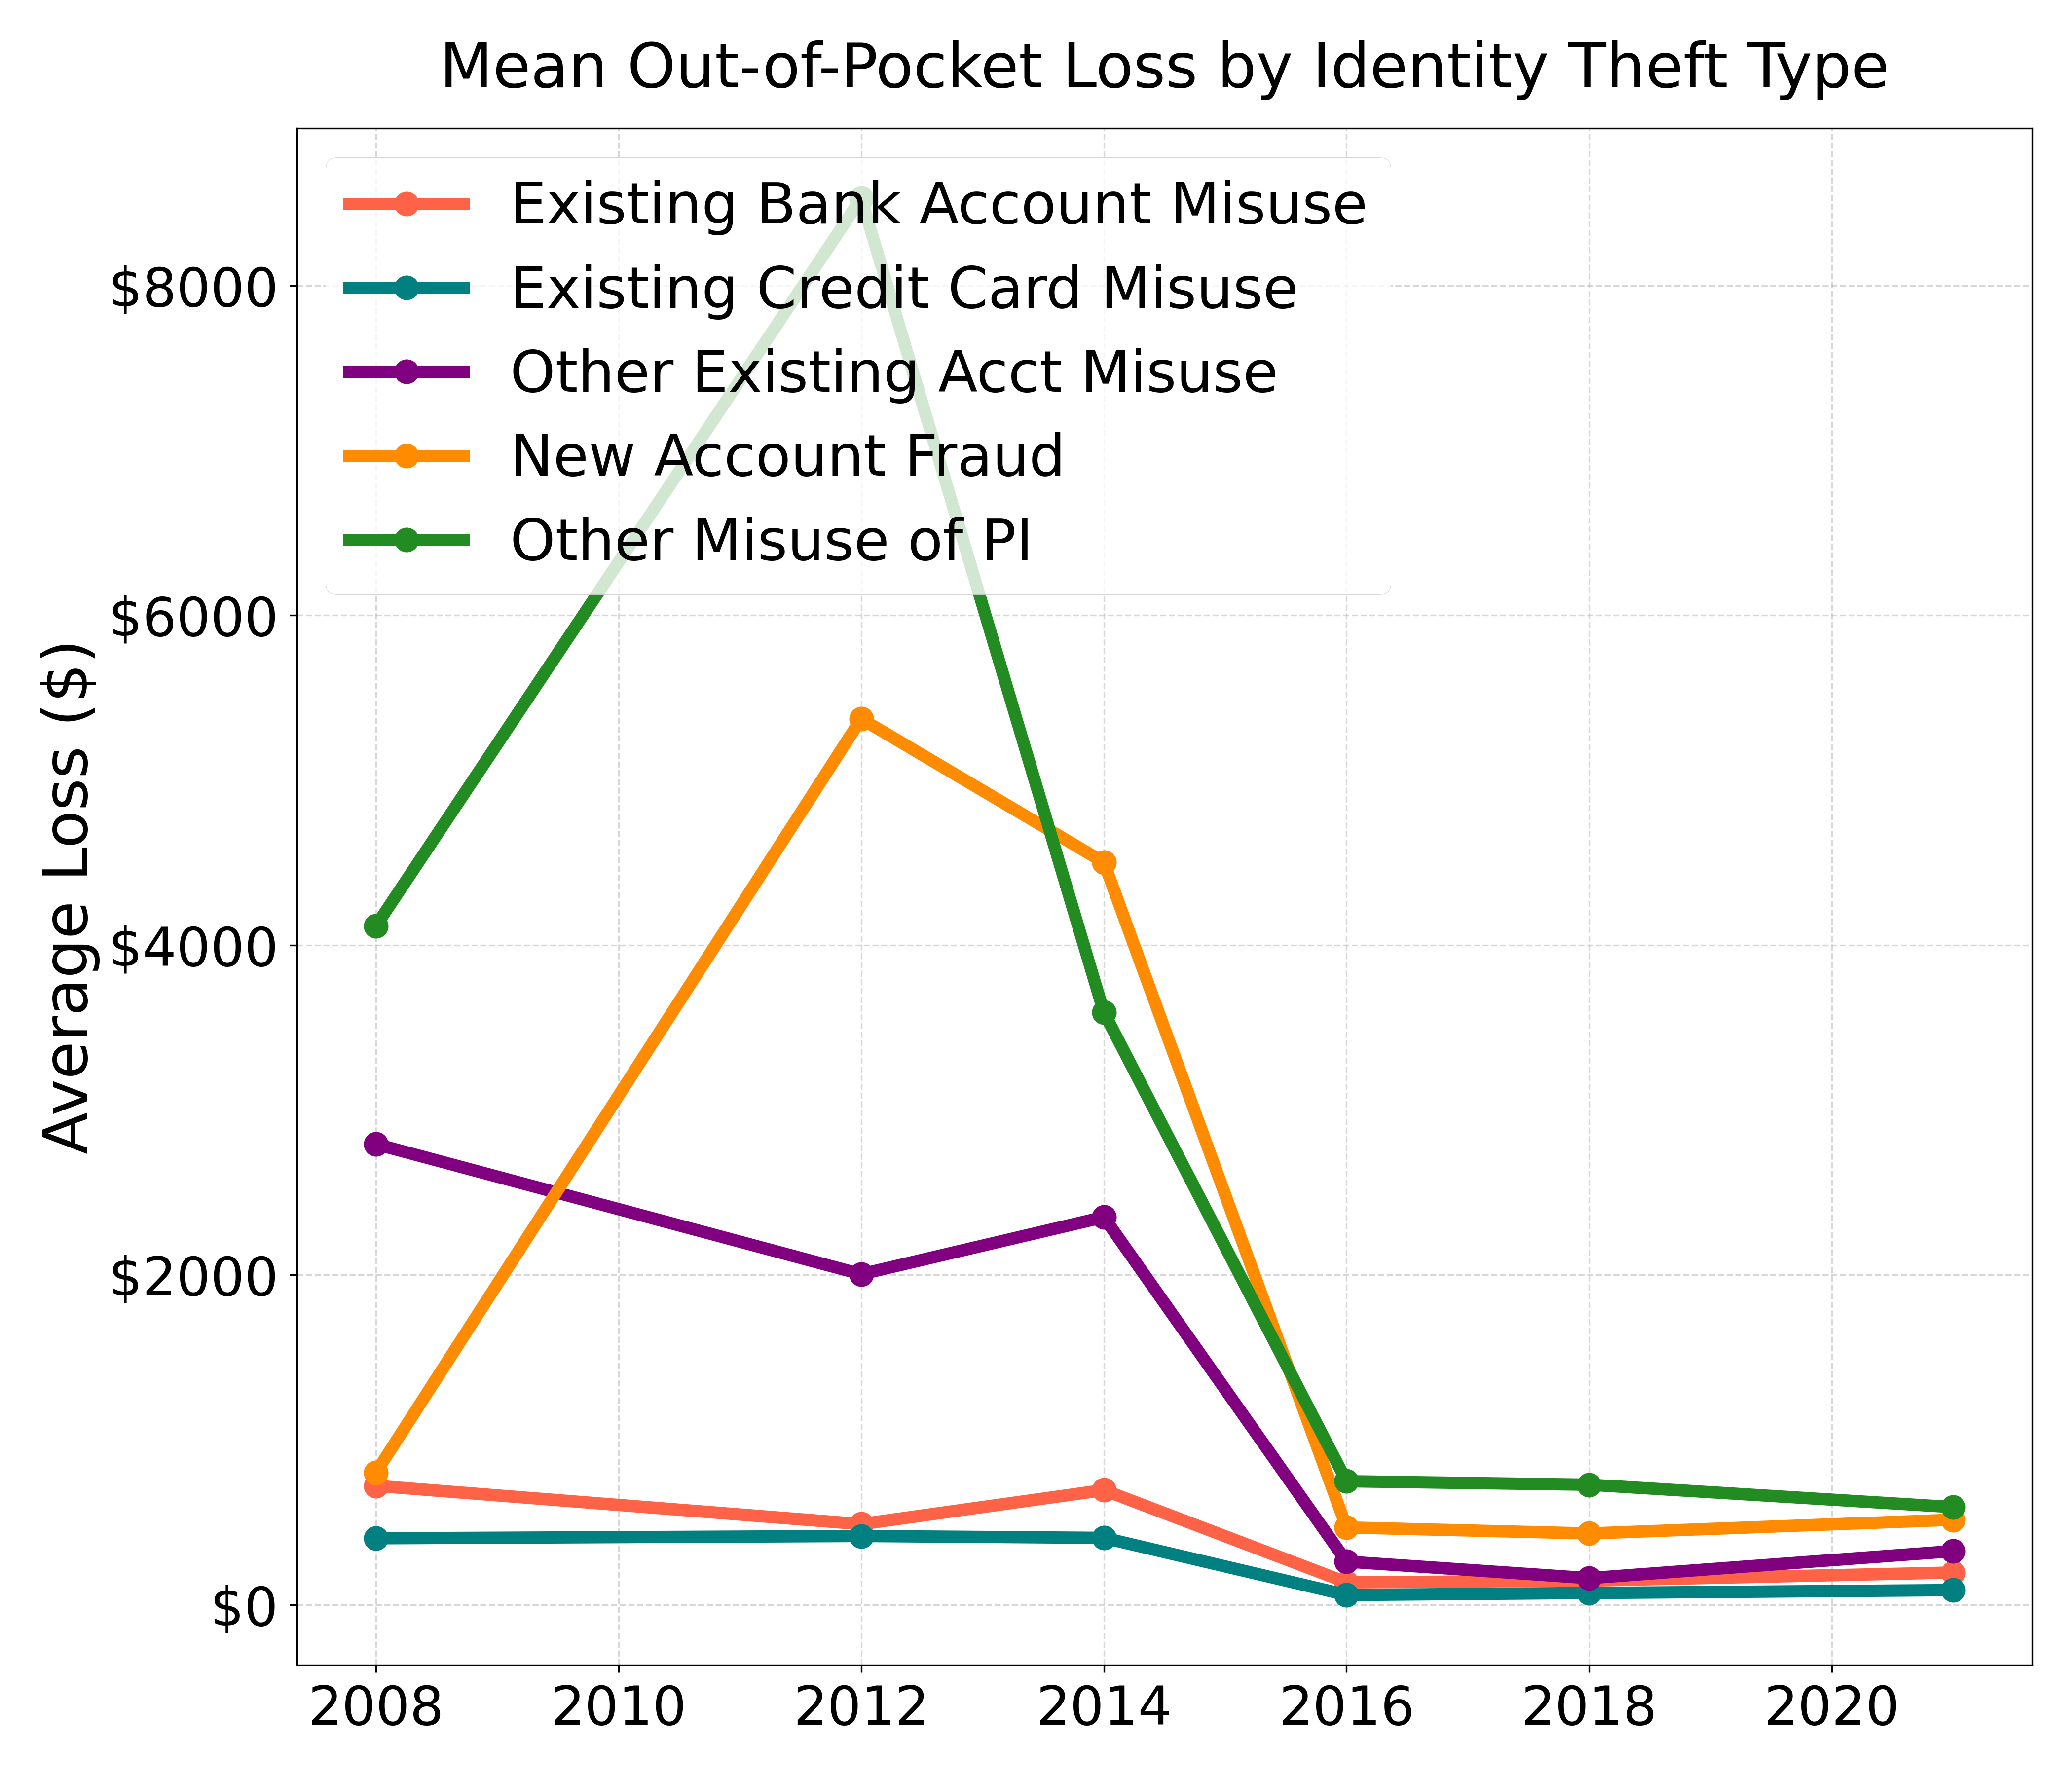
\includegraphics[width=0.48\textwidth]{figures/incident_trends/plot5_oop_loss_by_type.png}
%     \caption{Mean Out-of-Pocket Loss by Identity Theft Type (2008–2021).}
%     \label{fig:oop_loss_comparison}
% \end{wrapfigure}

Next, Figure \ref{fig:discovery_method_long} illustrates how victims became aware of the misuse, and its trends mirror the shift in crime types. "Notified by Bank," which rose significantly between 2008 and 2016 to become the most common discovery method (peaking at nearly 50\%), saw a sharp reversal, dropping considerably by 2021 to around 26\%. On the other hand, "Notified by Other Person/Organization," which began as a less common method, rose dramatically in 2021, increasing from roughly 6\% in 2018 to over 21\%. This aligns with the rise of social media and email account misuse as seen in Figure \ref{fig:theft_type_long}, suggesting victims are increasingly learning about compromises through their social networks or other non-financial organizations.


% \begin{figure}[htbp]
%     \centering
%     % --- Subfigure A: Counts ---
%     \begin{subfigure}[b]{0.48\textwidth}
%         \centering
%         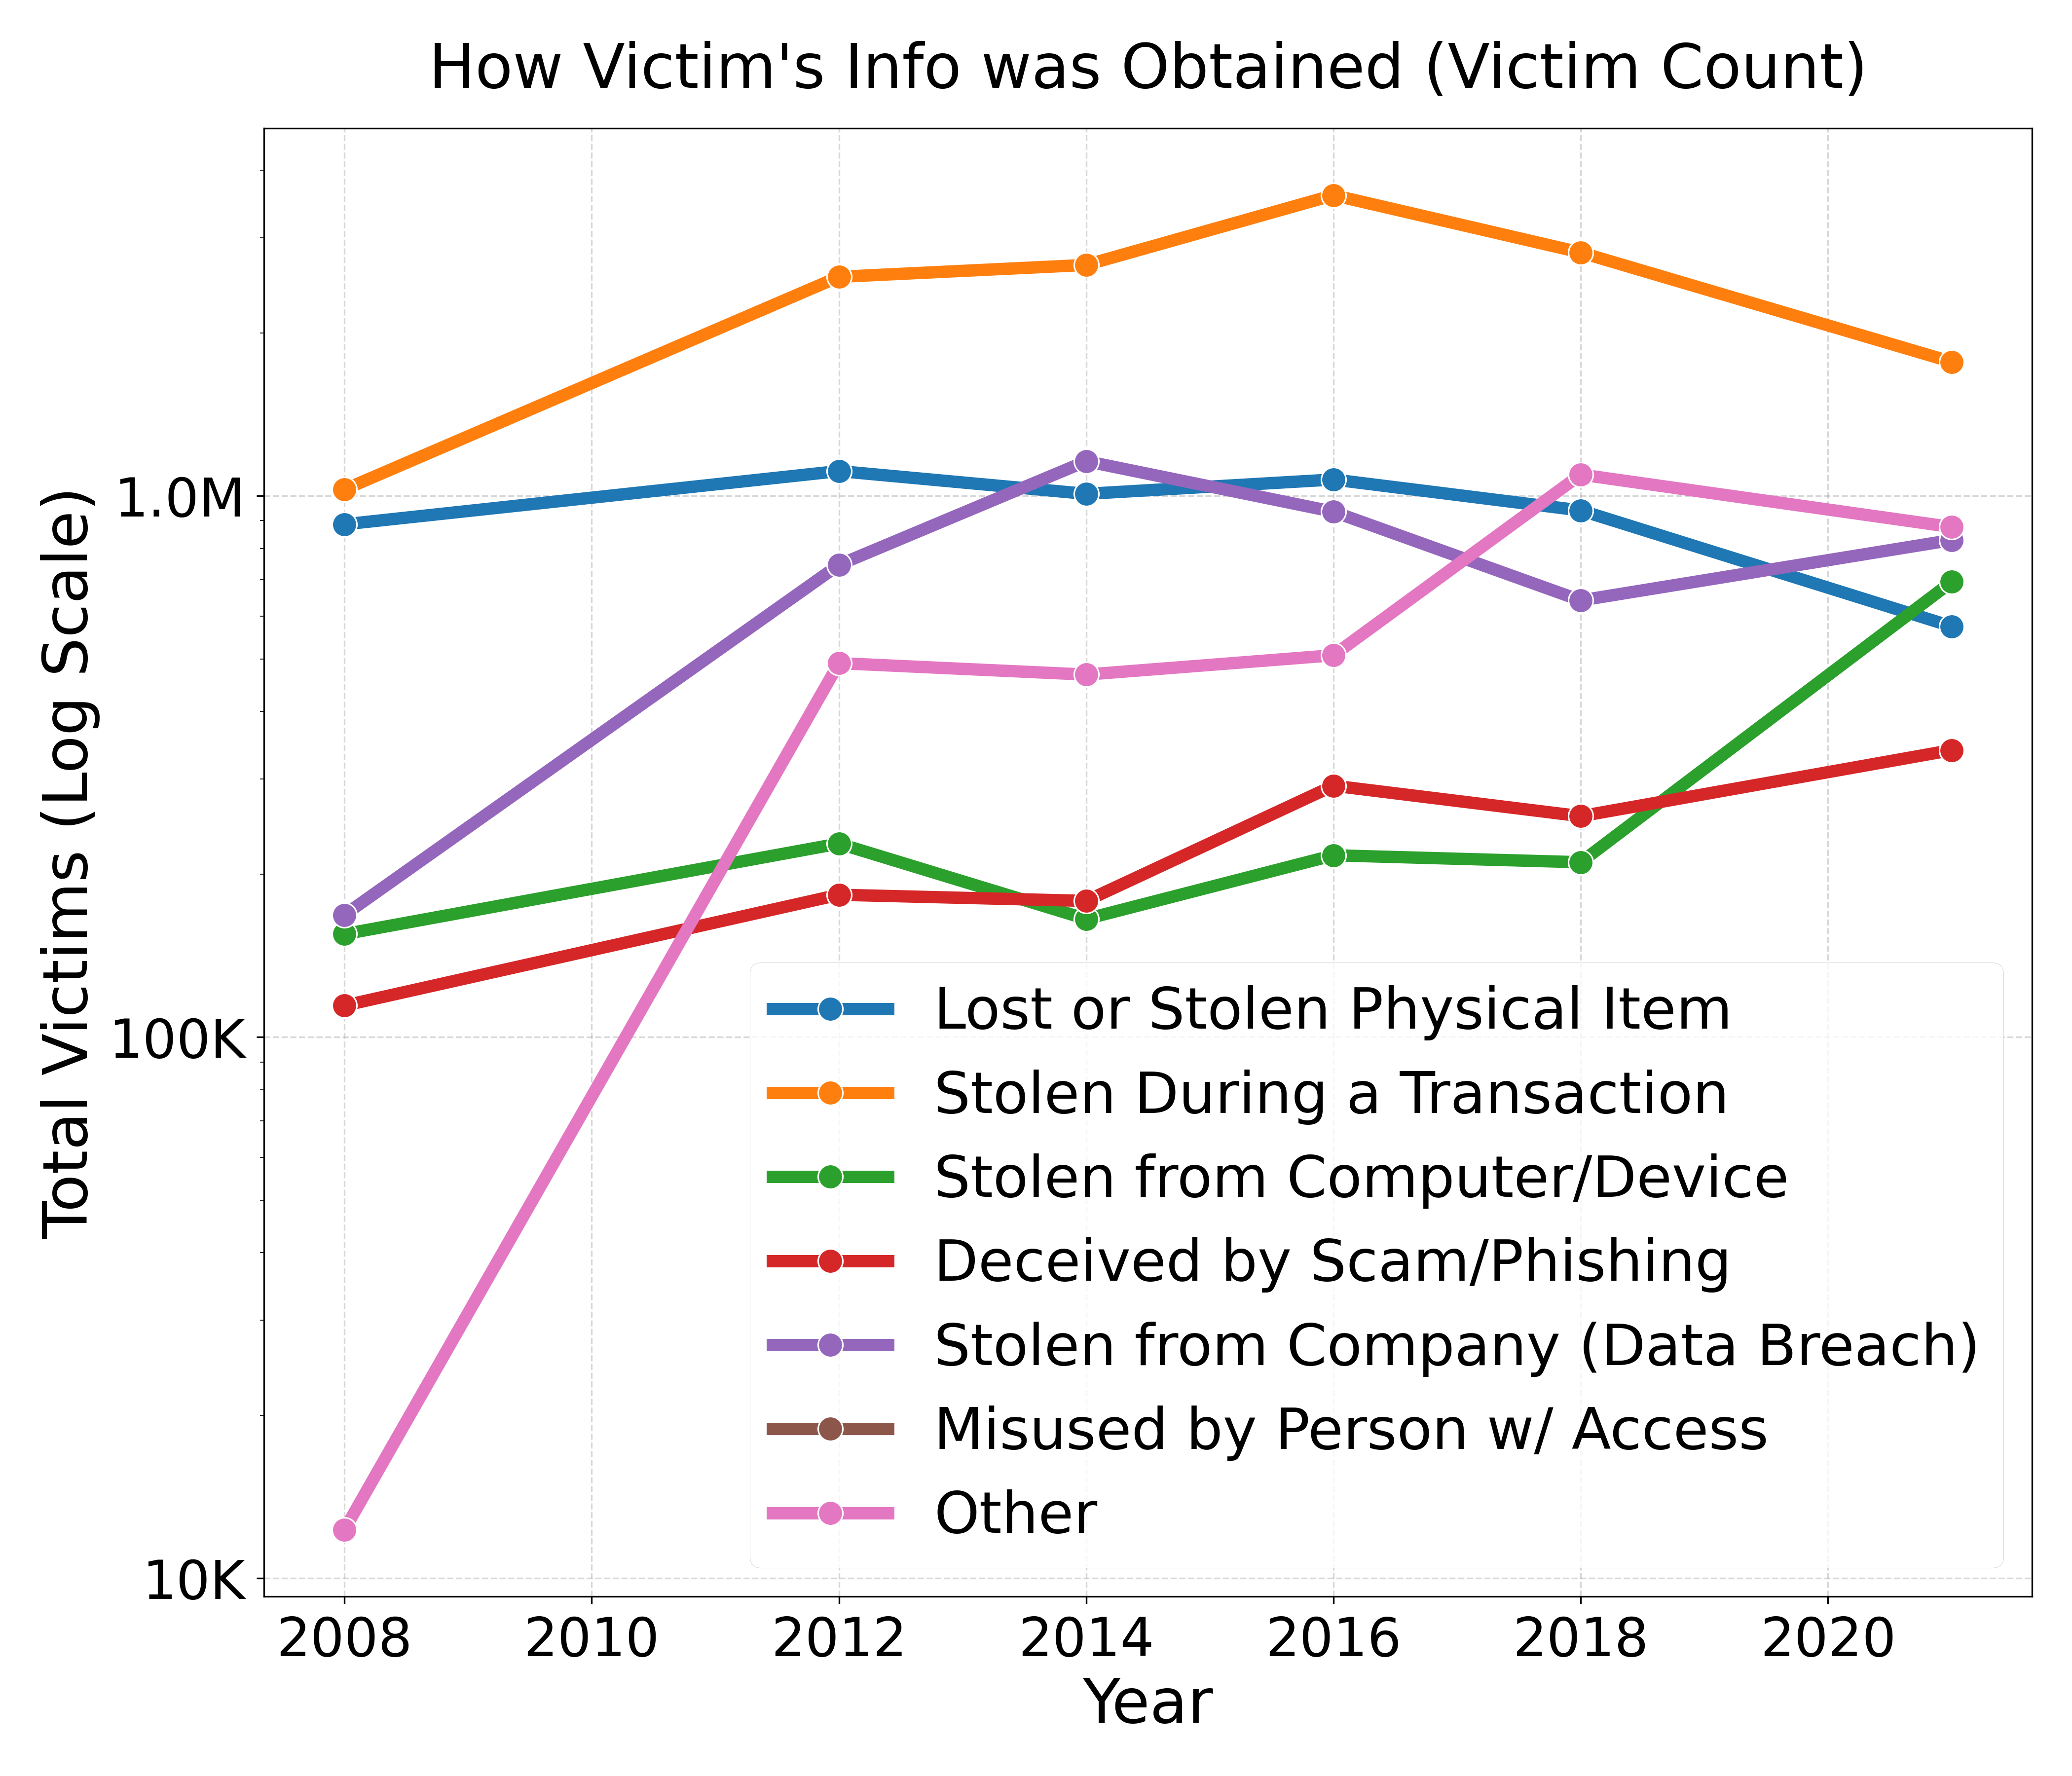
\includegraphics[width=\textwidth]{figures/incident_trends/plot1_theft_methods_count.png}
%         \caption{Number of victims categorized by how their information was stolen.}
%         \label{fig:theft_method_long_a}
%     \end{subfigure}
%     \hfill % Adds horizontal space between the two images
%     % --- Subfigure B: Percentages ---
%     \begin{subfigure}[b]{0.48\textwidth}
%         \centering
%         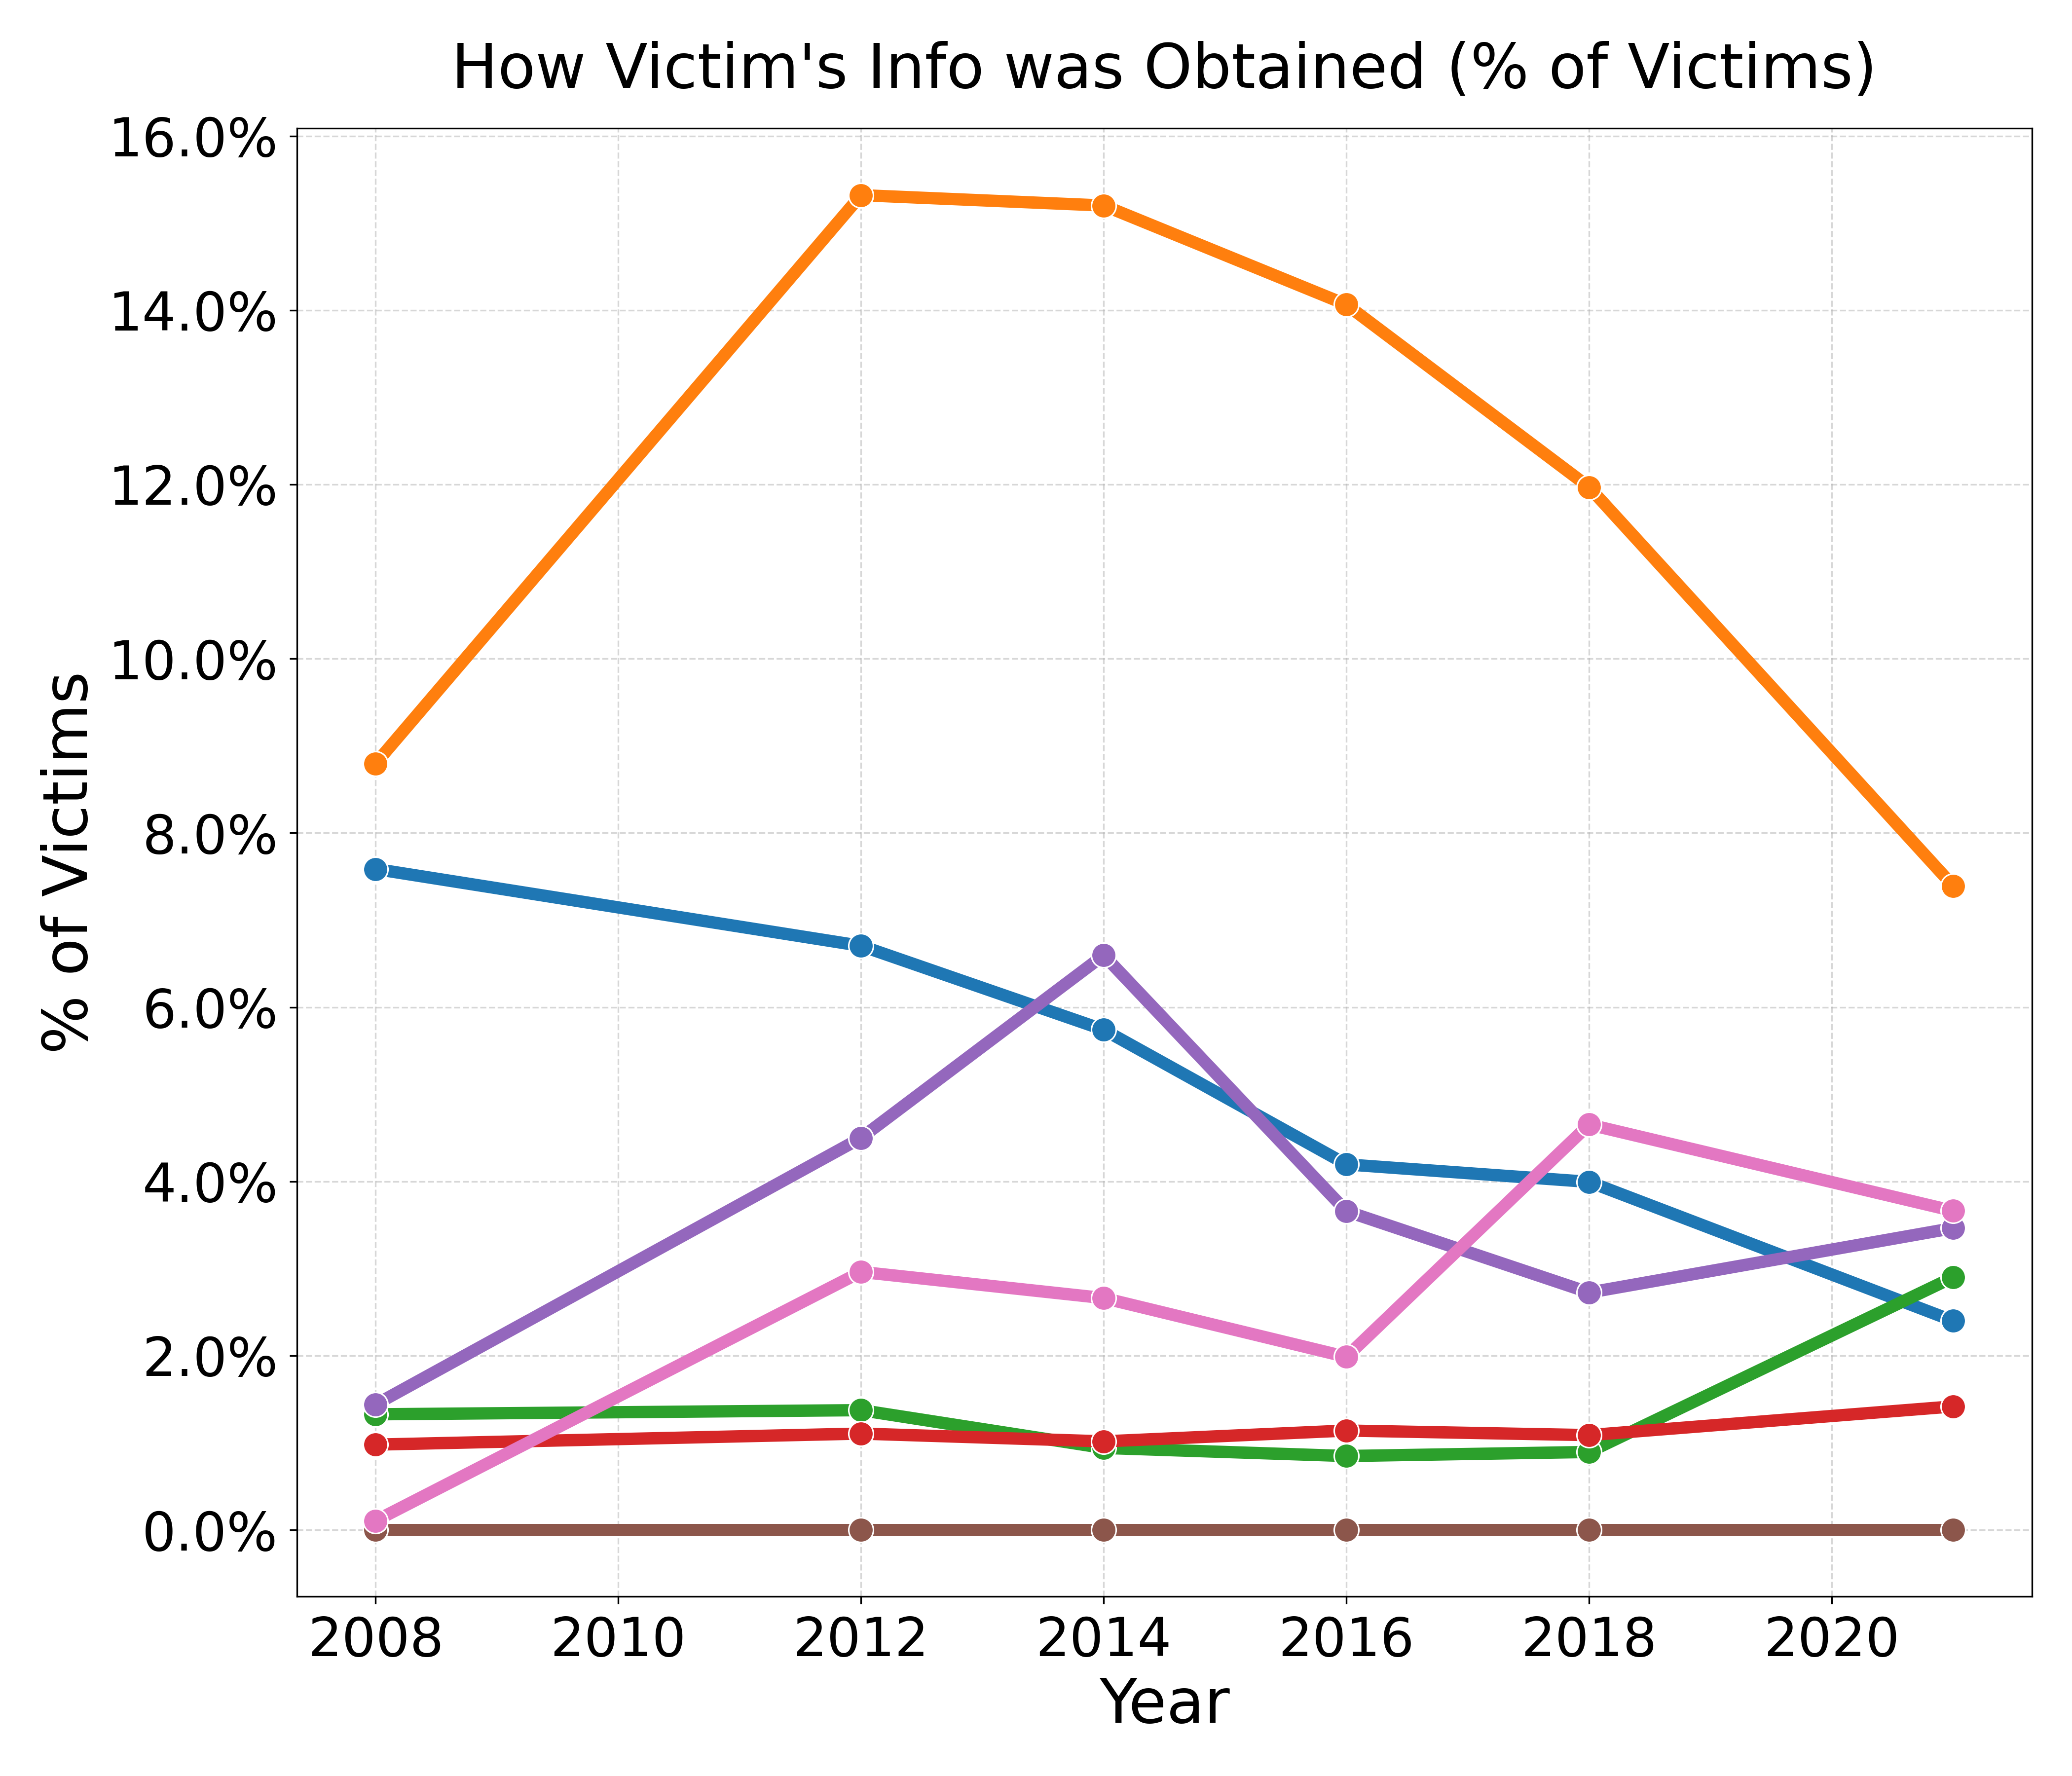
\includegraphics[width=\textwidth]{figures/incident_trends/plot1_theft_methods_percentage.png}
%         \caption{Percentage of victims categorized by how their information was stolen.}
%         \label{fig:theft_method_long_b}
%     \end{subfigure}
    
%     \caption{Analysis of theft methods over the longitudinal study period.}
%     \label{fig:theft_method_long}
% \end{figure}

\begin{figure}[htbp]
    \centering
    % --- Subfigure A: Counts ---
    \begin{subfigure}[b]{0.48\textwidth}
        \centering
        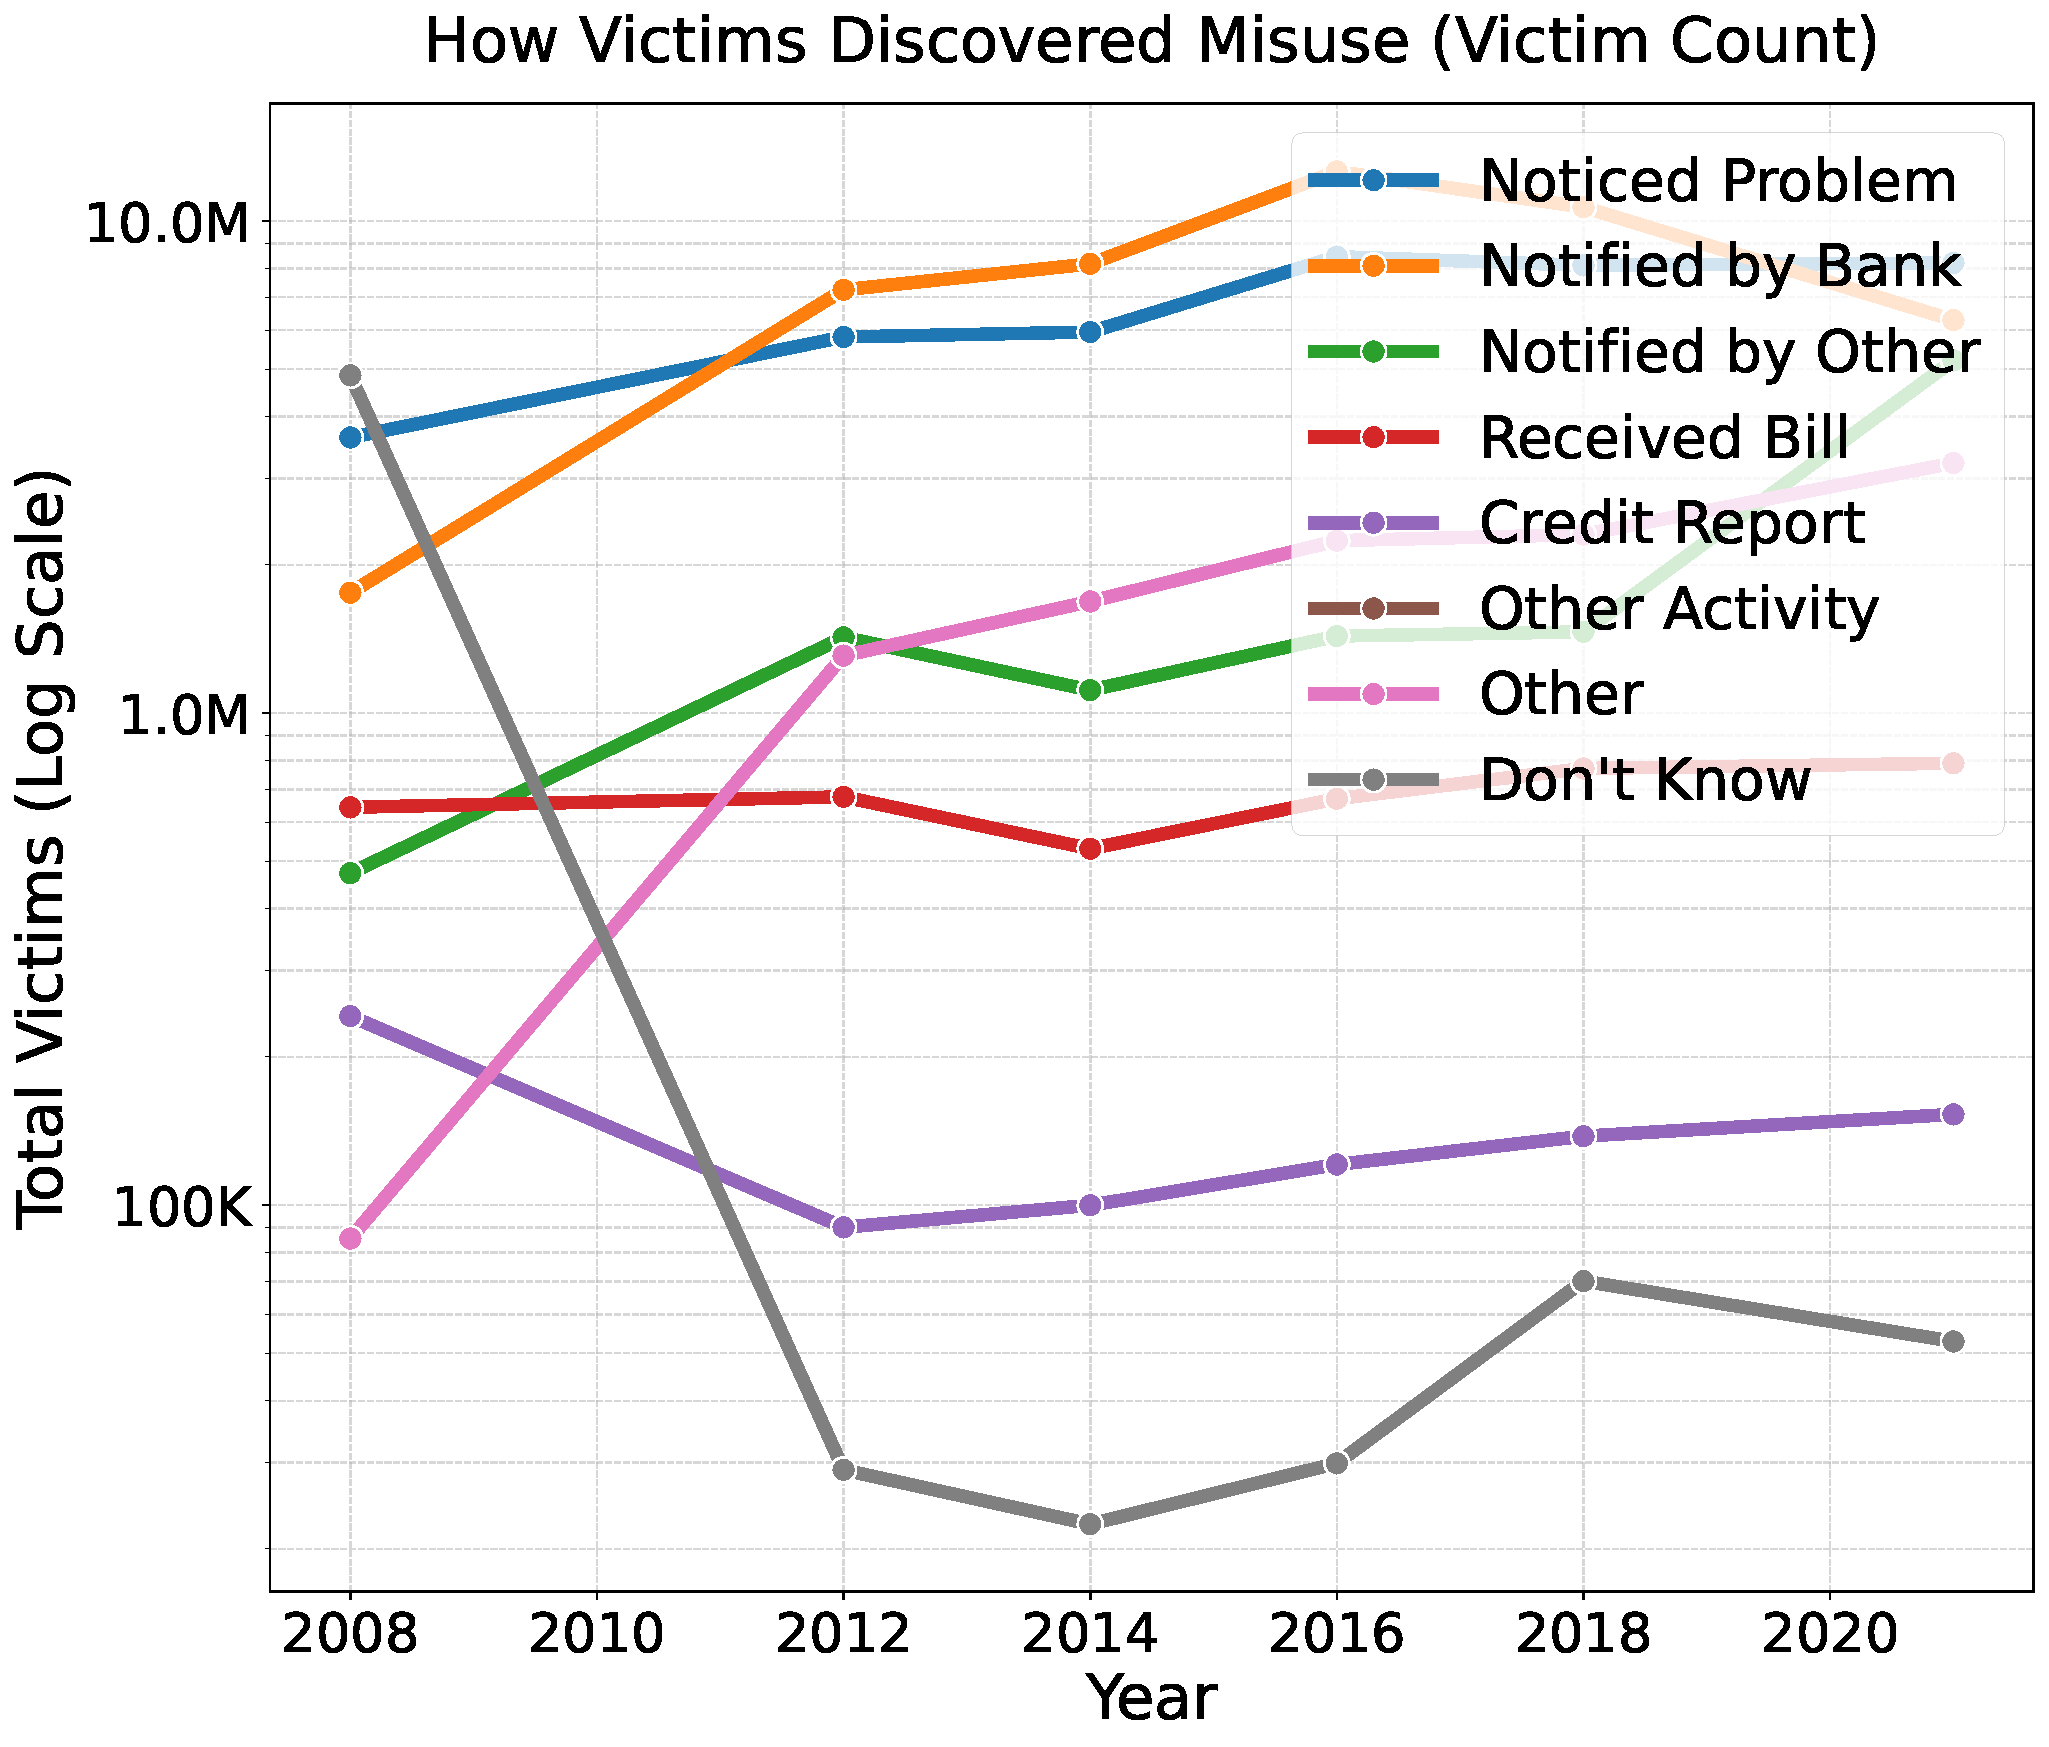
\includegraphics[width=\textwidth]{figures/incident_trends/plot3_discovery_count.pdf}
        \caption{Number of victims categorized by their discovery method.}
        \label{fig:discovery_method_long_a}
    \end{subfigure}
    \hfill
    % --- Subfigure B: Percentages ---
    \begin{subfigure}[b]{0.48\textwidth}
        \centering
        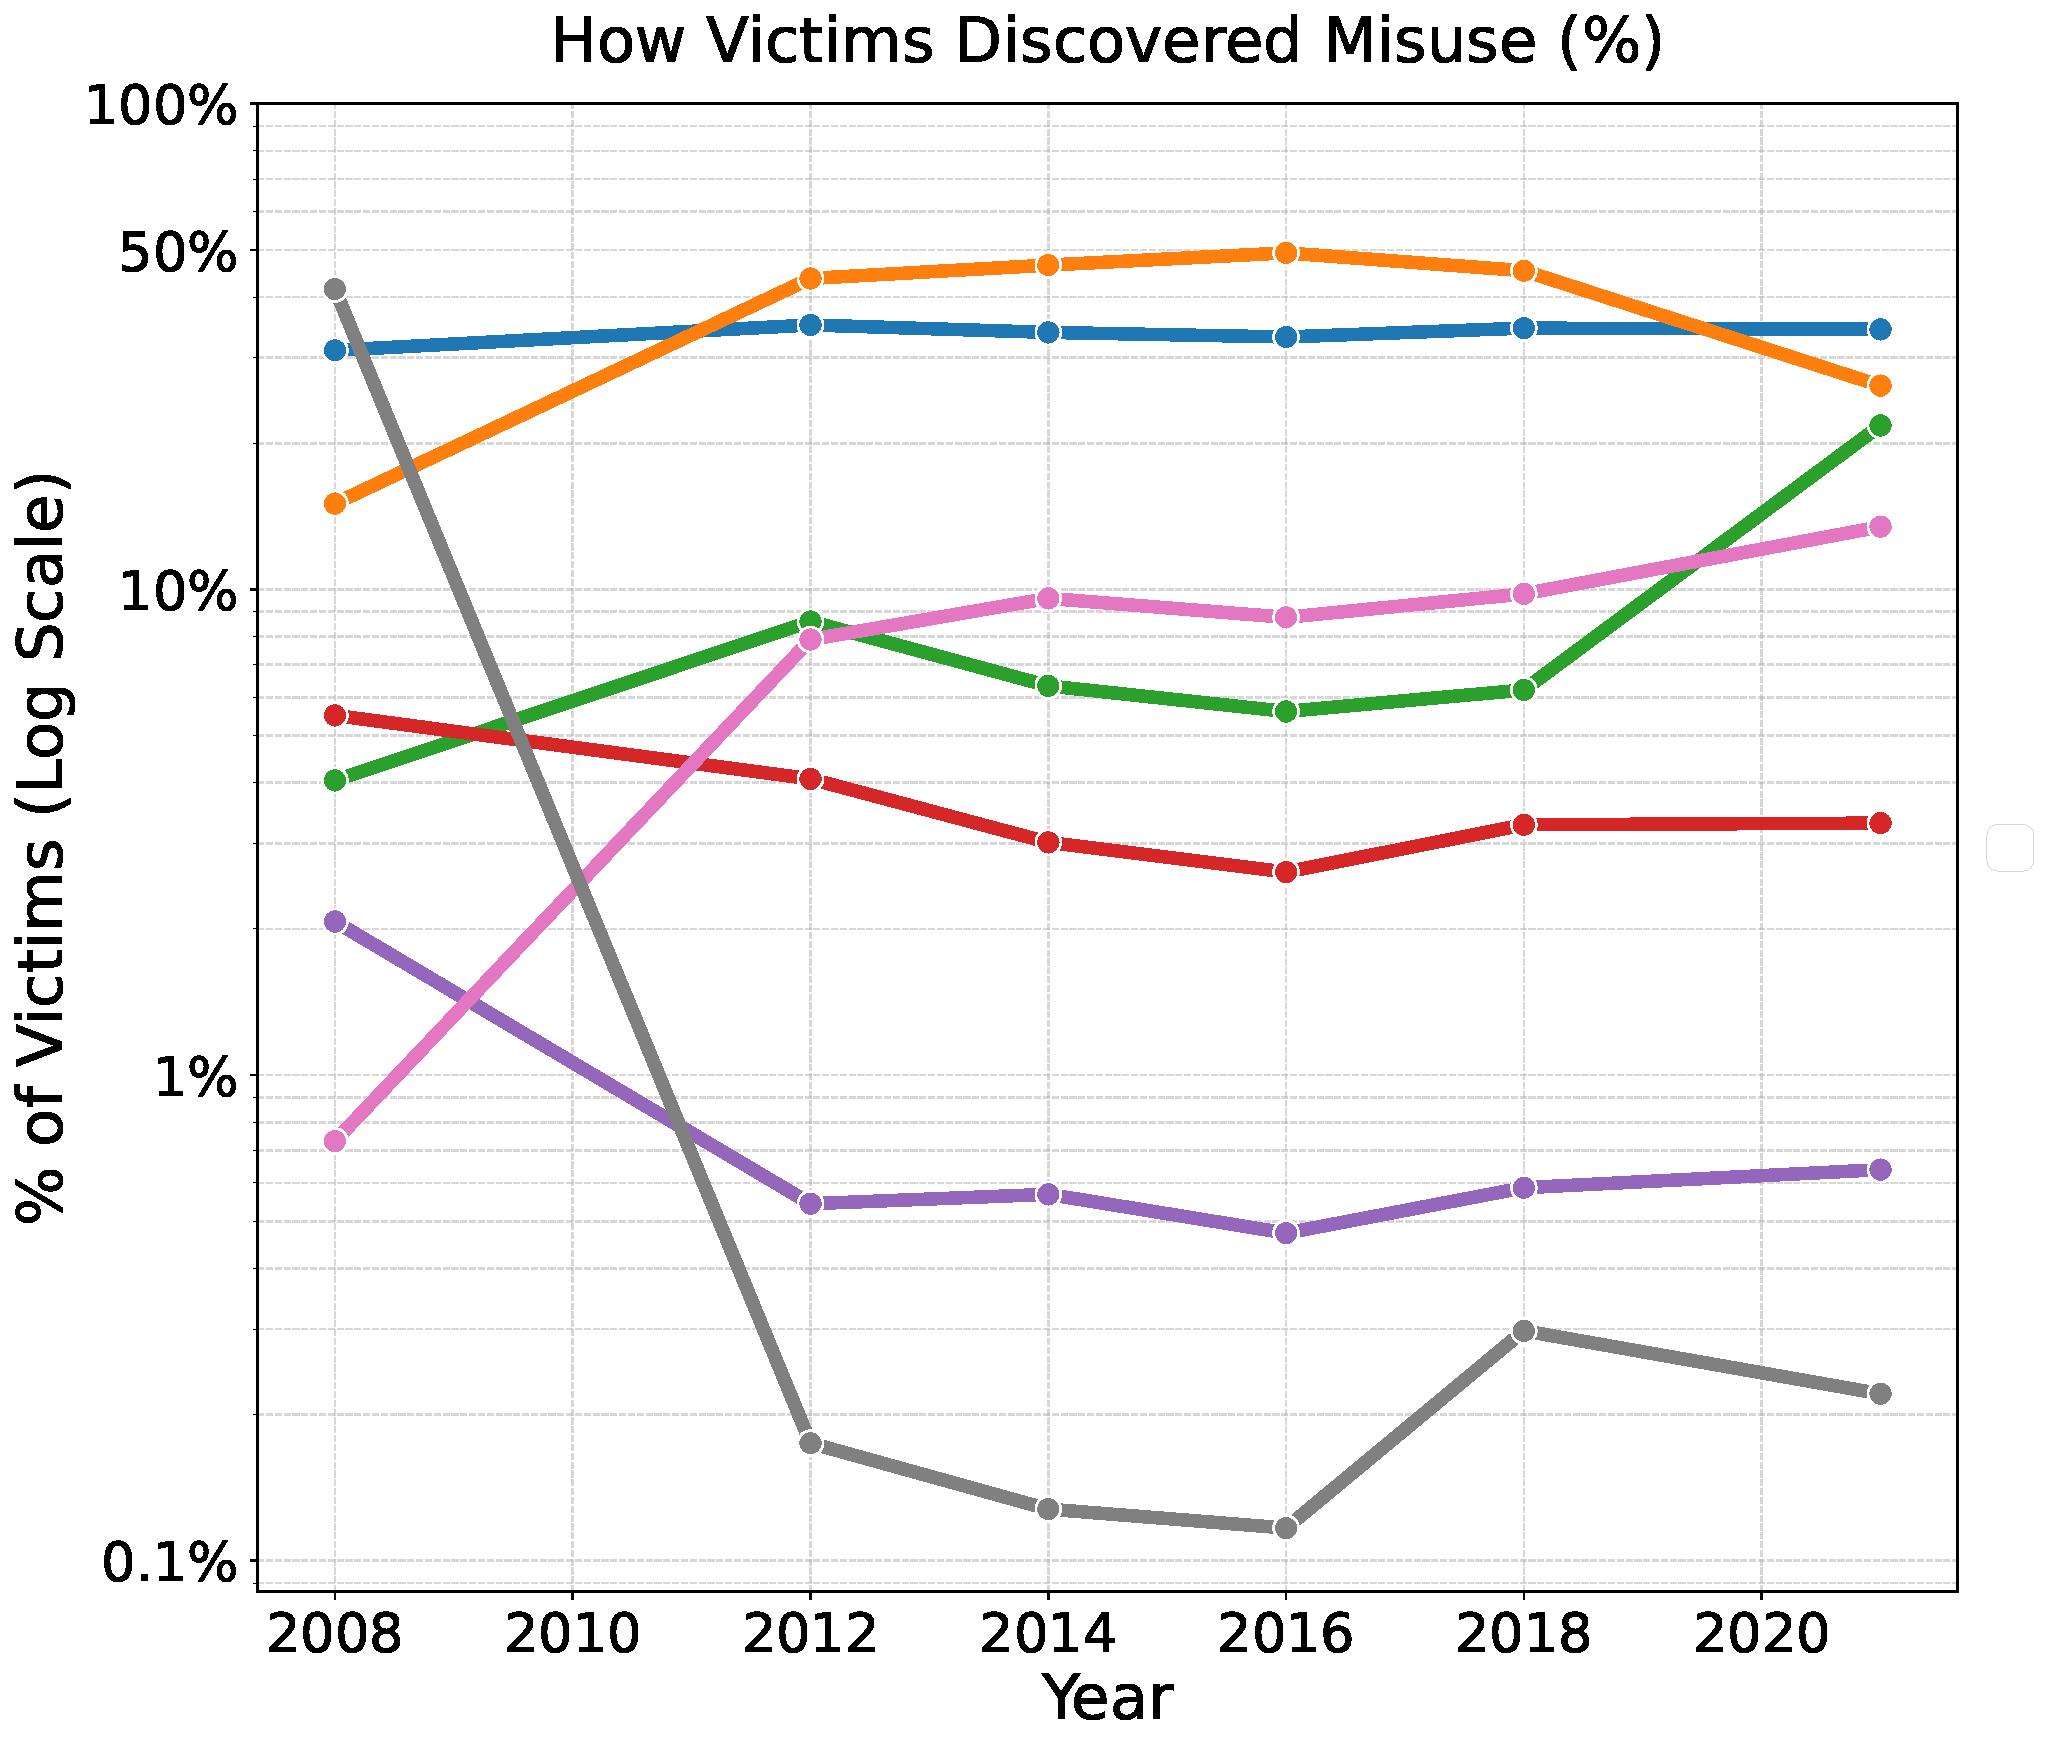
\includegraphics[width=\textwidth]{figures/incident_trends/plot3_discovery_percentage.pdf}
        \caption{Percentage of victims categorized by their discovery method.}
        \label{fig:discovery_method_long_b}
    \end{subfigure}
    
    \caption{Longitudinal trends in how victims discovered the theft incidents.}
    \label{fig:discovery_method_long}
\end{figure}


% Finally, a financial trend is evident in Figure \ref{fig:oop_loss_comparison}, which compares the average out of pocket (OOP) losses adjusted to 2021 dollars, specifically for victims of existing credit card misuse versus existing bank account misuse. It is worth noting that our OOP loss is less than direct loss values noted by BJS official reports \cite{HarrellThompson2024}, because we include only costs that were not recoverable to the victim, rather than including reimbursed costs. Both categories show a dramatic drop in average OOP loss between 2014 and 2016. Figure \ref{fig:oop_loss_comparison} displays that all categories show a dramatic drop and convergence between 2014 and 2016. We present two hypothesized explanations for this trend. 



% First, for the existing bank account misuse and existing credit card misuse OOP loss, the EMV transition could have played a role, because it reduced the most common type of high value, card present fraud, and for the fraud that did occur, liability was clearer and banks had implemented faster detection systems, leading to more \$0 liability outcomes for consumers \cite{aba2018report}. Victims still reported "credit card misuse" because criminals pivoted to online, card not present fraud \cite{fed2018fraud}. This remote fraud is often more easily and quickly reimbursed by banks. Unlike in-person counterfeit fraud, where a dispute could be complex, in a remote fraud case the victim is still in physical possession of their card, and bank systems can often use location data or IP addresses to quickly confirm the transaction was fraudulent. This shift to a more easily reimbursable type of fraud meant the number of victims in our survey experiencing a direct, unrecoverable OOP loss fell dramatically, pulling the average loss for the entire group down. The EMV mandate applied to both credit and debit cards, the latter of which are the primary driver of bank account fraud losses according to a report by the American Bankers Association \cite{aba2018report}. While EMV chips directly impacted counterfeit card fraud, the concurrent drop for bank accounts represents this debit card protection as well as other broader improvements in banks' fraud detection systems \cite{aba2018report}.   



% However, the fact that this drop is observed over all identity theft categories, including those unrelated to the EMV mandate, such as "Other Misuse of PI" and "New Account Fraud," suggests that the structural changes to the ITS survey during 2016 played a large role. In 2016, the survey underwent a sample redesign, where household sample sizes were increased by 41\%, and weights were recalibrated to reflect the 2010 Decennial Census \cite{Harrell2019Victims}. BJS mentions that these changes require caution when comparing 2016 estimates to previous waves \cite{Harrell2019Victims}. This survey shift likely explains the volatility seen in the "Other Misuse of PI" and "New Account Fraud" categories, which were characterized by lower incidence rates but potentially very high value outlier losses. The surge in mean loss for these types in 2012 and 2014 is likely due to a few extreme outlier cases that affect the smaller sample mean. The stabilization after 2016 suggests that the improved, larger scale sampling better diluted the impact of high loss outliers that previously skewed averages.
% \com{Both are sound and plausible explanations. Let's discuss when we next meet.}

\input{extended_version/extended_demographics}

\section{Detailed Data Demographics and Census Comparison}
\label{app:demographics_census}

Here we display a set of descriptive statistics for the combined dataset,  shown in Table \ref{tab:demographics_percent}, which provides an averaged demographic profile of victims and juxtaposes it against data for the general U.S. population from the Census Bureau. The Victim \% column reflects the characteristics of the sample of 41,091 victims from the harmonized data. To achieve this, the survey weights for victims within a specific category (for example, those aged 30-49 or holding a Bachelor's degree) were summed and then divided by the total weighted victim population. The result is an averaged demographic of a typical identity theft victim between 2008 and 2021. 

For the Census \% column, data was aggregated from several U.S. Census Bureau surveys corresponding to the ITS years (2008, 2012, 2014, 2016, 2018, and 2021). Race data was sourced from the American Community Survey (ACS) 1-Year Data Profile DP05 \cite{Census_ACS_DP05}, while household income data came from the Current Population Survey's (CPS) Table H-17 \cite{Census_CPS_H17}. The remaining categories of age, sex, and educational attainment were derived from ACS tables on U.S. age and sex composition \cite{Census_AgeSex}. The final percentages represent the average demographic makeup of the U.S. population across these years. Note that in this process, age related categories were aligned to ensure a valid comparison, because the ITS sample includes only individuals aged 16 or older. Thus, because ACS groups individuals aged 15-19, a proportional allocation of 80\% or four fifths of this group was used to estimate the 16-19 population. A similar adjustment was made for the educational attainment data where a 15-17 age bracket appeared, and two thirds of that population was taken to estimate the count for ages 16-17. 

\begin{longtable}{lrr}
\caption{Comparison of victim demographics to Census data (\%), averaged over 2008-2021.} \label{tab:demographics_percent} \\
\toprule
\textbf{Category} & \textbf{Victim \%} & \textbf{Census \%} \\
\midrule
\endfirsthead
\multicolumn{3}{c}%
{{\tablename\ \thetable{} -- continued from previous page}} \\
\toprule
\textbf{Category} & \textbf{Victim \%} & \textbf{Census \%} \\
\midrule
\endhead
\midrule
\multicolumn{3}{r}{{Continued on next page}} \\
\endfoot
\bottomrule
\endlastfoot
\multicolumn{3}{c}{\textbf{Age Group}} \\
\midrule
16-29 & 18.03 & 24.35 \\
30-49 & 38.25 & 33.32 \\
50-64 & 28.14 & 24.44 \\
65+ & 15.58 & 17.89 \\
\midrule
\multicolumn{3}{c}{\textbf{Victim Sex}} \\
\midrule
Male & 47.43 & 47.73 \\
Female & 52.57 & 52.27 \\
\midrule
\multicolumn{3}{c}{\textbf{Victim Race/Ethnicity}} \\
\midrule
White alone & 81.96 & 75.3 \\
Black or African American alone & 10.35 & 13.2 \\
Asian alone & 4.96 & 5.5 \\
American Indian/Alaska Native alone & 0.62 & 0.9 \\
Native Hawaiian/Pacific Islander alone & 0.29 & 0.2 \\
Two or More Races & 1.83 & 4.9 \\
\midrule
\multicolumn{3}{c}{\textbf{Victim Educational Attainment}} \\
\midrule
Less than High School & 5.60 & 15.17 \\
High School Graduate (or equivalent) & 18.12 & 28.38 \\
Some College/Associate Degree & 30.16 & 27.18 \\
Bachelor's Degree & 28.10 & 18.87 \\
Graduate/Professional Degree & 18.02 & 10.38 \\
\midrule
\multicolumn{3}{c}{\textbf{Victim Household Income}} \\
\midrule
Under \$15,000 & 5.78 & 8.32 \\
\$15,000 to \$24,999 & 5.46 & 7.95 \\
\$25,000 to \$49,999 & 19.92 & 19.12 \\
\$50,000 to \$74,999 & 18.26 & 15.78 \\
\$75,000 and over & 50.58 & 48.90 \\
\end{longtable}

Table \ref{tab:demographics_percent} provides several insights about the differences between the demographic profile of a victim versus the entire population. For example, adults aged 30-49 and 50-64, are overrepresented among victims compared to their share of the general population. Younger individuals aged 16-29 and seniors aged 65+ are underrepresented. This could suggest that identity theft disproportionately affects individuals who are in their prime working and earning years. On the other hand, victimization rates between sexes are remarkably aligned with the national population, suggesting that sex is not a significant differentiating factor in identity theft victimization. 

Table \ref{tab:demographics_percent} also highlights disparities in victimization rates across racial lines. White individuals are overrepresented among victims, making up 82\% of the victim population but only 75\% of the general population. In contrast, individuals of Black, Asian, American Indian or Alaskan Native descent, or of two or more races, are all underrepresented among victims. It is also noticeable that individuals with a Bachelor's degree or a Graduate/Professional degree are overrepresented among victims. For example, those with a graduate degree make up over 18\% of victims but only about 10\% of the census population. Those with a High school education or less are significantly underrepresented among victims. The impact of income is also shown, where households earning \$75,000 and over are slightly overrepresented, and  households in the lower income brackets (\$25,000 or less) are underrepresented. These disparities are further explored in \ref{app:underrep}.

\section{Analysis of Victimization Factors}
\label{app:underrep}

\subsection{Why are middle aged individuals (ages 30-64)  overrepresented among victims?}
The data indicates that individuals in their prime earning and working years are victimized at a higher rate than their younger and older counterparts. For instance, the 30-64 age bracket contains over 66\% of the victim population while representing less than 58\% of the general population. This overrepresentation may be due to a combination of their financial activity, the value they represent to criminals, and their patterns of digital purchasing. 

A testable hypothesis is that this demographic is "digitally active but not digitally native," meaning that vulnerability is a function of both digital nativity and digital activity. This suggests that while this middle aged group is highly active online for banking, work, and commerce, they may be more susceptible to sophisticated online scams (e.g. phishing) than younger, more "digitally native" generations who grew up with the technology. To investigate this hypothesis, a weighted proportions test was conducted using the harmonized dataset. This analysis required first isolating the age, theft method, and weight variables. Victims were categorized into the same age groups as in Table \ref{tab:demographics_percent}. To isolate the method of compromise, the theft method variable was filtered to only include unambiguous cases. This means that any theft method that is not clearly digital or physical was filtered out. This step was essential because some of the survey's categories are too broad for this analysis. For example, the category "Stolen during a transaction" is ambiguous, as it does not distinguish between an online transaction/digital theft and in in-person/physical theft. This category, along with the "Other" response was therefore excluded. 

This filtering process resulted in two mutually exclusive categories for analysis. The "Digital" group included victims whose information was obtained via "Stolen from a Computer/Device (Hacking)," "Deceived by a scam (e.g. Phishing)," and "Stolen from a Company/Employer (Data Breach)." The "Physical" group included victims whose information came from a "Lost or Stolen Physical Item (Wallet, Mail, etc.)." After filtering the dataset to these cases, a weighted proportions test, using the ITS weight variable, was run to compare the two age groups. Within each resulting cell (e.g., "16-29" and "Digital"), the final survey weights of all respondents were summed. This yielded a table of weighted totals, representing the estimated national count for each combination. Finally, the proportion of digital versus physical theft within each age group was calculated by dividing the weighted sum for each theft method by the total weighted sum for that age group. This process produces nationally representative proportions, allowing for accurate comparisons of victimization patterns across demographics.

\begin{table}[htbp]
  \centering % Center the table horizontally
  \caption{Weighted Proportion of Theft Method by Age Group.}
  \label{tab:age_theft_method} 
  \begin{tabular}{@{}lcc@{}} 
    \toprule
    \textbf{Age Group} & \textbf{Digital Theft (\%)} & \textbf{Physical Theft (\%)} \\
    \midrule
    16--29    & 44.7               & 55.3                \\
    30--49    & 58.5               & 41.5                \\
    50--64    & 63.4               & 36.6                \\
    65+       & 63.1               & 36.9                \\
    \bottomrule
  \end{tabular}
  \par 
  \vspace{0.5ex} 
  \small
 
\end{table}

The results of this analysis, shown in Table \ref{tab:age_theft_method}, support the hypothesis that middle aged individuals are digitally active but not digitally native." The proportion of victimization from digital methods is lowest for the 16-29 age group (44.7\%), which was the only age group more likely to be victimized by physical means (55.3\%). This suggests that being a digital native can lead to a degree of resilience to online scams. For all other age groups, the vulnerability to digital theft is high and similar. The 30-49 age group (58.5\%), 50-64 age group (63.4\%), and the 65+ age group (63.1\%) all show a vulnerability to digital compromise. This confirms that the non-digital native groups are more susceptible to these digital methods of theft. This finding, however, does not explain why the 65+ age group has a lower overall victimization rate. We theorize this is due to the second factor, the level of digital activity. The 30-64 age groups likely represent a unique target for criminals because they combine high vulnerability (not digitally native) with high activity (a larger digital footprint from banking, commerce, and work). The 65+ age group shares the same vulnerability, but likely has a smaller average digital footprint, presenting fewer targets for compromise. While this theory provides an explanation for the pattern seen in Table \ref{tab:demographics_percent}, it is a limitation of this study that the ITS dataset does not contain variables to directly measure digital activity. Therefore, we present this as our interpretation of our findings that warrants further research with more specialized data.


\subsection{Why are White individuals overrepresented among victims?}

While victimization occurs among all racial groups, the data shows that White individuals are victims at a rate higher than their share of the U.S. population (82\% of victims vs. 75\% of the census population). It is hypothesized that this disparity is a reflection of underlying socioeconomic variables. Overrepresentation of White individuals among victims may be due to them being overrepresented in the higher income and higher education brackets, which are also noted in the data as being groups with higher rates of victimization.

To explore this relationship more deeply, a series of weighted logistic regression models were developed using the full dataset including all survey respondents (not solely victims). The logistic regression models calculate Odds Ratios (OR), which quantify how the odds of being a victim change in relation to each predictor, relative to a baseline group. An OR that is greater than 1 indicates increased odds compared to the baseline, and vice versa. All models incorporated the final survey weight provided in the dataset to ensure findings generalize to the U.S. population, not just the sample characteristics. 

The primary predictor of interest was a binary indicator identifying respondents who reported their race solely as White versus all other respondents combined (who were the reference group). Additional control variables included categorical representations of the highest level of education completed and income, mirroring the groups in Table \ref{tab:demographics_percent}. Respondent age was also included as a continuous control variable in the third model. To integrate the categorical predictors for education and income into the regression, they were represented by sets of binary indicators. For each variable, one category was designated as a reference category ('Less than high school' for education, and 'Under than \$15,000' for income). These categories were chosen as they represent the lowest levels on their scales, providing a baseline against which to measure the effects of higher attainment or income.  Separate binary indicators then represented the remaining categories. This method allows the model coefficients to reflect the change in odds associated with belonging to a specific category relative to the baseline. Respondents missing any key variables were excluded, resulting in a sample of 544,837 individuals for these models.

Each model produces coefficients and corresponding p-values for each predictor. The p-value indicates statistical significance and indicates the probability of observing an association as strong as (or stronger than) the one found in the sample, if no true association existed in the population. A small p-value suggests that the observed relationship is unlikely due to random chance and is considered statistically significant. The modeling results are shown in Tables \ref{tab:logit_results}, \ref{tab:logit_age_results} and \ref{tab:race_profile_comparison}. In Table \ref{tab:logit_results}, the initial model ("Race Only"), containing only the White race indicator, confirmed that identifying as White was associated with significantly higher odds of victimization (OR = 1.320, p $<$ 0.001), compared to non-White respondents.

\begin{table}[htbp]
  \centering
  \begin{threeparttable}
  \caption{Weighted Logistic Regression Predicting Likelihood of Identity Theft Victimization.}
  \label{tab:logit_results}
  % Apply small font size to the entire table content
  \small
  % Adjust siunitx setup
  \sisetup{
    table-format=1.3,
    table-align-text-post=false,
    table-number-alignment=center,
    input-comparators = <, % Define < as an input comparator
    table-sign-comparator = true, % Use < > >= <= signs
    round-mode=places,
    round-precision=3 % Ensure p-values round correctly
  }
  % Reduce inter-column spacing slightly
  \setlength{\tabcolsep}{4pt}
  \begin{tabular}{@{} l
                     S[table-format=1.3] S[table-format=<1.3] @{\hspace{2pt}} % Use table-format=<1.3 directly
                     S[table-format=1.3] S[table-format=<1.3] @{\hspace{2pt}}
                     S[table-format=1.3] S[table-format=<1.3] @{\hspace{2pt}}
                     S[table-format=1.3] S[table-format=<1.3]
                     @{}}
    \toprule
    & \multicolumn{2}{c}{\textbf{Race Only}} & \multicolumn{2}{c}{\textbf{+ SES Controls}} & \multicolumn{2}{c}{\textbf{+ SES + Age}} & \multicolumn{2}{c}{\textbf{+ Interaction (Race*Edu})} \\
    \cmidrule(lr){2-3} \cmidrule(lr){4-5} \cmidrule(lr){6-7} \cmidrule(lr){8-9}
    Predictor & {OR} & {p} & {OR} & {p} & {OR} & {p} & {OR} & {p} \\
    \midrule
    \textbf{Race} & & & & & & & & \\
    \quad White (Ref: Non-White) & 1.320 & <0.001 & 1.268 & <0.001 & 1.257 & <0.001 & 1.048 & 0.427 \\
    \addlinespace
    \textbf{Education} (Ref: $<$ HS) & & & & & & & & \\
    \quad HS Graduate & & & 1.954 & <0.001 & 1.928 & <0.001 & 1.630 & <0.001 \\
    \quad Some College/Assoc. & & & 3.173 & <0.001 & 3.144 & <0.001 & 2.930 & <0.001 \\
    \quad Bachelor's & & & 3.852 & <0.001 & 3.809 & <0.001 & 3.085 & <0.001 \\
    \quad Graduate/Professional & & & 4.743 & <0.001 & 4.654 & <0.001 & 3.812 & <0.001 \\
    \addlinespace
    \textbf{Income} (Ref: $<$ \$15k) & & & & & & & & \\
    \quad \$15k -- \$24,999 & & & 1.002 & 0.963 & 0.995 & 0.867 & 1.004 & 0.895 \\
    \quad \$25k -- \$49,999 & & & 1.024 & 0.349 & 1.021 & 0.420 & 1.028 & 0.289 \\
    \quad \$50k -- \$74,999 & & & 1.188 & <0.001 & 1.187 & <0.001 & 1.192 & <0.001 \\
    \quad \$75k and over & & & 1.366 & <0.001 & 1.369 & <0.001 & 1.371 & <0.001 \\
    \addlinespace
    \textbf{Age} & & & & & & & & \\
    \quad Age & & & & & 1.002 & <0.001 & & \\
    \addlinespace
    \textbf{Interaction: White*Edu} & & & & & & & & \\
    \quad White * HS Grad & & & & & & & 1.245 & 0.002 \\
    \quad White * Some College & & & & & & & 1.105 & 0.122 \\
    \quad White * Bachelor's & & & & & & & 1.305 & <0.001 \\
    \quad White * Graduate & & & & & & & 1.301 & <0.001 \\
    \addlinespace
    \midrule
    % Pseudo R-squared & \multicolumn{2}{S[table-format=0.3]}{0.001} & \multicolumn{2}{S[table-format=0.3]}{0.031} & \multicolumn{2}{S[table-format=0.3]}{0.031} & \multicolumn{2}{S[table-format=0.3]}{0.031} \\
    % Log-Likelihood & \multicolumn{2}{S[table-format=-1.3e+1]}{-1.376e+05} & \multicolumn{2}{S[table-format=-1.3e+1]}{-1.336e+05} & \multicolumn{2}{S[table-format=-1.3e+1]}{-1.335e+05} & \multicolumn{2}{S[table-format=-1.3e+1]}{-1.335e+05} \\
    N (Respondents, in thousands) & \multicolumn{2}{S[table-format=6.0, table-space-text-pre=(]}{544,837} & \multicolumn{2}{S[table-format=6.0]}{544,837} & \multicolumn{2}{S[table-format=6.0]}{544,837} & \multicolumn{2}{S[table-format=6.0]}{544,837} \\
    \bottomrule
  \end{tabular}
    \begin{tablenotes}[para,flushleft] % Make notes paragraph style
      \small % Ensure notes match table font size
      \item \textit{Note:} Table displays odds ratios (OR) and p-values (p) from weighted logistic regressions. SES = Socioeconomic Status (Income and Education). Edu = Education. HS = High School. Assoc. = Associate Degree.
      Reference category for Race is Non-White. Reference category for Education is Less than High School ($<$ HS). Reference category for Income is Under \$15,000 ($<$ \$15k). $p$-values less than 0.001 are shown as "$<$0.001".
      Models used final survey weights. 
    \end{tablenotes}
  \end{threeparttable}
\end{table}

The second model ("+SES controls") added indicators for education and income levels. Adding these control variables allows the model to statistically isolate the specific association between the primary predictor (the White race indicator) and the outcome (victimization), while holding the influence of these other factors constant. The odds ratio for the White race indicator decreased in this model (OR = 1.268), which is consistent with the hypothesis that socioeconomic factors contribute to the disparity. This reduction confirms that education and income differences account for some, but not all, of the initial race based difference.

The third model, ("+SES, + Age") incorporated the respondent's age. The odds ratio for the White race indicator reduced slightly again (OR = 1.257), but stayed highly significant (p$<$0.001). This finding strengthens the conclusion that race maintains an independent association with victimization risk, beyond what can be explained by education, income, and age differences. Age itself also emerged as having a small, statistically significant positive relationship with victimization odds (OR=1.002, p$<$0.001) in this model. 

The final model, ("+Interaction (Race*Edu)") tested whether the relationship between education and victimization risk differs systematically for White versus non-White individuals. This involved adding interaction terms to the model. An interaction term tests if the effect of one predictor (like having a Bachelor's degree) depends on, or is modified by, the level of another predictor (like being White). Creating these interaction terms involves mathematically combining the indicators for the two variables in question. In our analysis code, this was done by multiplying the binary indicator for being White (0 or 1) by the binary indicator for each specific education level (0 or 1). The resulting term (e.g., "White * Bachelor's") will only equal 1 if a person is both White and has a Bachelor's degree; otherwise, it is 0. By including these combined terms in the regression, the model can estimate this joint effect separately from the individual effects of race and education alone.

This fourth model yielded the most interesting findings. The main effect associated with the White race indicator (representing the effect of being White compared to non-White specifically among those in the reference education group, 'Less than High School') became non significant (OR = 1.048, p = 0.427). However, several interaction terms were statistically significant (e.g., White * HS Grad: OR = 1.245, p = 0.002; White * Bachelor's: OR = 1.305, p $<$ 0.001). These results refute the initial hypothesis that race serves only as a proxy for socioeconomic status. The analysis reveals a significant interaction, which is the way educational attainment relates to the odds of identity theft victimization is different for White individuals compared to non-White individuals. The positive interaction odds ratios suggest that higher levels of education correspond to a greater increase in victimization risk for White respondents than for non-White respondents, relative to those with less than a high school education. This relationship requires deeper examination than originally anticipated.

Regarding the observation that most odds ratios in Table \ref{tab:logit_results} are above 1, this simply reflects the patterns in the data relative to the chosen reference groups. For education and income, the higher categories consistently show increased odds of victimization compared to the lowest categories ('Less than High School' and 'Under \$15,000'). Similarly, the initial models showed White individuals had higher odds than non-White individuals. Odds ratios close to 1 (like those for the lower middle income brackets, which are not statistically significant) indicate little difference in odds compared to the reference group. An odds ratio significantly less than 1 would indicate lower odds of victimization, but such a pattern was not observed for most primary predictors in these models. A similar analysis was done for Tables \ref{tab:logit_age_results} and \ref{tab:race_profile_comparison}, where Table \ref{tab:race_profile_comparison} performs a comparative profile analysis that measures the percentage of each reported category with respect to race.

\begin{table}[htbp]
  \centering
  \begin{threeparttable}
  \caption{Weighted Logistic Regression Predicting Likelihood of Identity Theft Victimization by Age Group.}
  \label{tab:logit_age_results}
  % Apply small font size to the entire table content
  \small
  % Adjust siunitx setup
  \sisetup{
    table-format=1.3,
    table-align-text-post=false,
    table-number-alignment=center,
    input-comparators = <, % Define < as an input comparator
    table-sign-comparator = true, % Use < > >= <= signs
    round-mode=places,
    round-precision=3 % Ensure p-values round correctly
  }
  % Reduce inter-column spacing slightly
  \setlength{\tabcolsep}{4pt}
  \begin{tabular}{@{} l
                     S[table-format=1.3] S[table-format=<1.3] @{\hspace{2pt}} % Age Only
                     S[table-format=1.3] S[table-format=<1.3] @{\hspace{2pt}} % + SES Controls
                     S[table-format=1.3] S[table-format=<1.3] % + Full Controls
                     @{}}
    \toprule
    & \multicolumn{2}{c}{\textbf{Age Only}} & \multicolumn{2}{c}{\textbf{+ SES Controls}} & \multicolumn{2}{c}{\textbf{+ SES/Race Controls}} \\
    \cmidrule(lr){2-3} \cmidrule(lr){4-5} \cmidrule(lr){6-7}
    \textbf{Predictor} & {OR} & {p} & {OR} & {p} & {OR} & {p} \\
    \midrule
    \textbf{Age Group (Ref: 65+)} & & & & & & \\
    \quad 16-29 & 0.722 & <0.001 & 0.817 & <0.001 & 0.836 & <0.001 \\
    \quad 30-49 & 1.312 & <0.001 & 1.149 & <0.001 & 1.176 & <0.001 \\
    \quad 50-64 & 1.319 & <0.001 & 1.210 & <0.001 & 1.223 & <0.001 \\
    \addlinespace
    \textbf{Education (Ref: $<$ HS)} & & & & & & \\
    \quad HS Graduate & {} & {} & 1.845 & <0.001 & 1.842 & <0.001 \\
    \quad Some College/Assoc. & {} & {} & 3.016 & <0.001 & 3.009 & <0.001 \\
    \quad Bachelor's & {} & {} & 3.585 & <0.001 & 3.629 & <0.001 \\
    \quad Graduate/Professional & {} & {} & 4.322 & <0.001 & 4.429 & <0.001 \\
    \addlinespace
    \textbf{Income (Ref: $<$ \$15k)} & & & & & & \\
    \quad \$15k -- \$24,999 & {} & {} & 0.997 & 0.916 & 0.986 & 0.653 \\
    \quad \$25k -- \$49,999 & {} & {} & 1.022 & 0.389 & 1.005 & 0.848 \\
    \quad \$50k -- \$74,999 & {} & {} & 1.180 & <0.001 & 1.154 & <0.001 \\
    \quad \$75k and over & {} & {} & 1.341 & <0.001 & 1.311 & <0.001 \\
    \addlinespace
    \textbf{Race (Ref: Other)} & & & & & & \\
    \quad White & {} & {} & {} & {} & 0.827 & <0.001 \\
    \quad Black & {} & {} & {} & {} & 0.673 & <0.001 \\
    \quad Asian & {} & {} & {} & {} & 0.500 & <0.001 \\
    \midrule
    N (Respondents, in thousands) & \multicolumn{2}{c}{544.837} & \multicolumn{2}{c}{544.837} & \multicolumn{2}{c}{544.837} \\
    \bottomrule
  \end{tabular}
    \begin{tablenotes}[para,flushleft] % Make notes paragraph style
      \small % Ensure notes match table font size
      \item \textit{Note:} Table displays odds ratios (OR) and p-values (p) from weighted logistic regressions. Model 1 includes only Age Group. Model 2 adds Socioeconomic Status (SES: Income and Education). Model 3 adds Race (White, Black, Asian) to the controls. Reference category for Age Group is 65+. Reference categories for Income and Education are as follows: Income is Under \$15,000; Education is Less than High School. Race reference is 'Other' (Non-White, Non-Black, Non-Asian). $p$-values less than 0.001 are shown as "$<$0.001". Models used final survey weights. 
    \end{tablenotes}
  \end{threeparttable}
\end{table}


\begin{table}[htbp]
  \centering
  \begin{threeparttable}
  \caption{Victim Profile Comparison: Theft and Discovery Methods by Race (Weighted \%)}
  \label{tab:race_profile_comparison}
  \small % Use a smaller font size to ensure fit

  \begin{tabular}{@{} l *{4}{R} *{3}{P} @{}}
  
    \toprule
    \textbf{Category} & \multicolumn{4}{c}{\textbf{Weighted \% of Victims in Group}} & \multicolumn{3}{c}{\textbf{Difference vs. All Other (pp)}} \\
    \cmidrule(lr){2-5} \cmidrule(lr){6-8}
     & {White} & {Black} & {Asian} & {All Other} & {Diff} & {Diff} & {Diff} \\
     & {(\%)} & {(\%)} & {(\%)} & {(\%)} & {(White)} & {(Black)} & {(Asian)} \\
    \midrule
    \multicolumn{8}{@{} l}{\textbf{Type of Identity Theft}} \\
    \midrule
    Existing Bank Account Misuse & 40.89 & 54.03 & 27.01 & 51.89 & -11.00 & +2.14 & -24.87 \\
    Existing Credit Card Misuse & 49.81 & 28.01 & 64.55 & 31.12 & +18.69 & -3.11 & +33.43 \\
    Other Existing Account Misuse & 12.48 & 17.25 & 12.61 & 18.20 & -5.72 & -0.95 & -5.59 \\
    New Account Fraud & 6.52 & 12.77 & 6.31 & 12.30 & -5.78 & +0.46 & -5.99 \\
    Other Misuse of PI & 5.21 & 8.54 & 3.85 & 6.15 & -0.95 & +2.39 & -2.30 \\
    \midrule
    \multicolumn{8}{@{} l}{\textbf{How Misuse Was Discovered}} \\
    \midrule
    Problem with Account & 33.18 & 36.51 & 36.85 & 37.92 & -4.74 & -1.41 & -1.07 \\
    Notified by Bank & 40.86 & 28.65 & 39.04 & 31.24 & +9.62 & -2.59 & +7.80 \\
    Notified by Other  & 9.02 & 12.03 & 7.21 & 13.23 & -4.21 & -1.20 & -6.02 \\
    Checked Credit Report & 0.57 & 1.89 & 0.45 & 1.34 & -0.78 & +0.55 & -0.89 \\
    Other/Unspecified & 8.74 & 12.19 & 9.59 & 9.13 & -0.38 & +3.06 & +0.46 \\
    Don't Know & 0.00 & 0.00 & 0.00 & 0.00 & +0.00 & +0.00 & +0.00 \\
    \midrule
    \multicolumn{8}{@{} l}{\textbf{How Information Was Obtained}} \\
    \midrule
    Lost or Stolen Physical Item & 4.20 & 8.71 & 4.13 & 6.84 & -2.65 & +1.87 & -2.71 \\
    Stolen During Transaction & 12.45 & 9.92 & 10.22 & 13.36 & -0.91 & -3.43 & -3.13 \\
    Hacking/Computer Theft & 1.34 & 1.53 & 1.56 & 2.43 & -1.09 & -0.90 & -0.88 \\
    Data Breach (Company/Employer) & 3.79 & 3.46 & 3.41 & 4.74 & -0.95 & -1.28 & -1.33 \\
    Other & 2.78 & 3.85 & 1.88 & 4.71 & -1.93 & -0.86 & -2.83 \\
    \bottomrule
  \end{tabular}
  \begin{tablenotes}
    \item \textit{Note}: Table displays weighted percentage profiles of victims by racial group. "All Other Victims" includes American Indian/Alaska Native, Native Hawaiian/Pacific Islander, Two or More Races, and Latino groups, and serves as the reference category. Categories for theft type may sum to $>100\%$ as victims can experience multiple types of fraud.
  \end{tablenotes}
  \end{threeparttable}
\end{table}



\subsection{Why are individuals with higher educational attainment and income overrepresented among victims?}

% \com{I have to say this question jumps out at me as being the most significant: the race/age/income related disparity in representation pales by comparison to education related disparity..}

The data also shows that individuals with higher socioeconomic status (individuals with more education or higher education levels) are overrepresented in the victim sample. For example, individuals with a graduate or professional degree make up 18\% of victims but only 10\% of the general population. In addition, Table \ref{tab:logit_results} revealed a strong association between education and likelihood of victimization. Even after controlling for race, age, and income, as education level increased, the odds ratio of becoming a victim increased as well. Having a graduate or professional degree was especially notable, being associated with an odds ratio of 4.743, meaning those individuals are almost five times as likely to be victims. This suggests that they could be more attractive or accessible targets for criminals.

One prominent hypothesis suggests that these individuals represent more valuable targets due to potentially greater assets, higher credit limits, and larger savings. An alternative but not mutually exclusive hypothesis is that these individuals might have a larger digital and commercial footprint, thereby creating more opportunities for their data to be compromised. 

This analysis focused on testing the "More to steal" hypothesis by examining whether higher socioeconomic status correlates with greater financial losses among those who experienced identity theft. The initial, most intuitive step was to calculate the simple weighted average out of pocket loss for victims in each education and income category. The results of this analysis, presented in Table \ref{tab:weighted_avg_loss}, were counterintuitive. They appeared to contradict the hypothesis, showing that the highest average losses were borne by victims in the lowest socioeconomic groups, such as those with less than a high school education (\$414.96) and those earning under \$15,000 (\$565.86).

% --- Table 3.4a: Weighted Averages ---
\begin{table}[htbp]
  \centering
  \begin{threeparttable}
  \caption{Weighted Average Out-of-Pocket Loss per Victim by Socioeconomic Group}
  \label{tab:weighted_avg_loss}
  \begin{tabular}{@{} l S[table-format=3.2] @{}}
    \toprule
    \textbf{Category} & {\textbf{Weighted Average Loss (\$)}} \\
    \midrule
    \multicolumn{2}{@{}l}{\textbf{Education Level}} \\
    \hspace{1em} Less than High School & 414.96 \\
    \hspace{1em} High School Graduate & 281.56 \\
    \hspace{1em} Some College/Assoc. Degree & 309.63 \\
    \hspace{1em} Bachelor's Degree & 166.51 \\
    \hspace{1em} Graduate/Professional Degree & 213.25 \\
    \midrule
    \multicolumn{2}{@{}l}{\textbf{Income Level}} \\
    \hspace{1em} Under \$15,000 & 565.86 \\
    \hspace{1em} \$15,000 to \$24,999 & 412.49 \\
    \hspace{1em} \$25,000 to \$49,999 & 439.74 \\
    \hspace{1em} \$50,000 to \$74,999 & 250.81 \\
    \hspace{1em} \$75,000 and over & 128.05 \\
    \bottomrule
  \end{tabular}
    \begin{tablenotes}[para,flushleft]
      \small
      \item \textit{Note:} Table displays the simple weighted average out-of-pocket loss for victims.
    \end{tablenotes}
  \end{threeparttable}
\end{table}

To further explore potential reasons why individuals with higher educational attainment are overrepresented, a comparative profile analysis was also conducted. Using the victim-only data, respondents were segmented into three mutually exclusive groups based on their highest education level: Graduate/Professional, Bachelor's Degree, and All Other Victims. The average weighted percentage for each type of theft, discovery method, and theft method was then calculated for each of these three groups. The results are presented in Table \ref{tab:victim_profile_education}. The most significant finding in Table \ref{tab:victim_profile_education} is a dramatic difference in the type of fraud experienced. Both high education groups are far more likely to be victims of Existing Credit Card Misuse. The Bachelor's Degree group experiences this fraud at a rate of 18.39\% higher than the baseline group, while the Graduate/Professional group's rate is 27.53\% higher than the baseline. This finding is mirrored by Existing Bank Account Misuse, where both high education groups are underrepresented (13.43 and 21.93\% lower than baseline, respectively). This strongly suggests that the high victimization odds ratio observed in the regression models is driven mainly by credit card fraud, not attacks on debit cards or bank accounts. This is further explained by the findings on discovery methods. Both the Bachelor's Degree and Graduate/Professional groups were significantly more likely to be notified by a financial institution (7.30 and 9.43\% higher than baseline, respectively). They also were less likely to have noticed a problem with their accounts themselves.

\begin{table}[htbp]
  \centering
  \begin{threeparttable}
  \caption{Victim Profile Comparison by Education Level}
  \label{tab:victim_profile_education}
  
  % Setup for siunitx columns
  \sisetup{
    table-align-text-post=false,
    round-mode=places,
    round-precision=2
  }
  
  % l = left-aligned text column
  % S[...] = numeric columns aligned by decimal
  \begin{tabular}{@{} l
                     S[table-format=2.2]
                     S[table-format=2.2]
                     S[table-format=2.2]
                     S[table-format=+2.2]
                     S[table-format=+2.2] @{}}
    \toprule
    Category & {Grad./Prof.} & {Bach.'s} & {All Other} & {(Grad - Other)} & {(Bach. - Other)} \\
             & {(\%)}           & {(\%)}              & {(\%)}              & {(\%)}            & {(\%)}            \\
    \midrule
    
    % --- Type of Theft ---
    \multicolumn{6}{@{}l}{\textbf{Type of Identity Theft}} \\
    \quad Existing Bank Account    & 27.62 & 36.12 & 49.55 & -21.93 & -13.43 \\
    \quad Existing Credit Card     & 65.29 & 56.16 & 37.76 &  27.53 &  18.39 \\
    \quad Other Existing Account   & 12.28 & 12.64 & 13.61 &  -1.34 &  -0.97 \\
    \quad New Account Fraud              & 6.15  & 6.25  & 8.17  &  -2.02 &  -1.92 \\
    \quad Other Misuse  & 5.22  & 4.47  & 6.04  &  -0.82 &  -1.57 \\
    \quad Multiple Types                 & 14.72 & 14.23 & 13.24 &   1.48 &   0.99 \\
    \addlinespace % Adds a little vertical space

    % --- Discovery Method ---
    \multicolumn{6}{@{}l}{\textbf{How Misuse Was Discovered}} \\
    \quad  Problem with Account     & 29.76 & 32.00 & 36.18 & -6.42 & -4.19 \\
    \quad Notified by Bank & 45.02 & 42.89 & 35.59 &  9.43 &  7.30 \\
    \quad Notified by Other    & 8.95  & 8.74  & 9.74  & -0.79 & -1.00 \\
    \quad Received Bill Not Ordered   & 2.94  & 3.01  & 3.82  & -0.88 & -0.81 \\
    \quad Checked Credit Report            & 0.45  & 0.63  & 0.84  & -0.40 & -0.22 \\
    \quad Other/Unspecified                & 9.10  & 8.99  & 9.15  & -0.05 & -0.16 \\
    \quad Don't Know                     & 0.15  & 0.09  & 0.10  &  0.05 & -0.01 \\
    \addlinespace % Adds a little vertical space

    % --- Theft Method ---
    \multicolumn{6}{@{}l}{\textbf{How Info Was Obtained}} \\
    \quad Lost/Stolen Physical Item   & 3.43  & 3.81  & 5.56  & -2.13 & -1.75 \\
    \quad  During Transaction      & 11.91 & 12.45 & 12.12 & -0.21 &  0.33 \\
    \quad Hacking/Computer Theft         & 1.39  & 1.27  & 1.50  & -0.11 & -0.23 \\
    \quad Scam/Phishing      & 1.08  & 0.93  & 1.29  & -0.21 & -0.36 \\
    \quad Data Breach  & 4.11  & 4.05  & 3.51  &  0.60 &  0.54 \\
    \quad Other                          & 1.91  & 2.20  & 3.59  & -1.68 & -1.39 \\
    
    \bottomrule
  \end{tabular}
    \begin{threeparttable}
      \small
    \end{threeparttable}
  \end{threeparttable}
\end{table}

This indicates that the overrepresentation of high education individuals as victims could be due to them having a heavier reliance on credit cards, which are a high-volume target for fraud. Their high odds of victimization in the survey are likely a function of their increased exposure to this specific fraud type, and the real-time fraud detection systems that credit card companies use. This effective monitoring means that frauds against this group are more likely to be detected and reported to the victim, thus captured by the survey.


\section{Social Cost by Demographic Group}

\subsection{Demographic Disparities in Social Cost}

While our detailed demographic analysis in Appendix \ref{app:demographics} showed that high socio-economic status (SES) individuals have higher odds of victimization, the social cost results shown in Figures \ref{fig:social_cost_age}, \ref{fig:social_cost_race}, \ref{fig:social_cost_education}, and \ref{fig:social_cost_income} demonstrate that the severity of the burden falls disproportionately on vulnerable populations. In terms of age, the highest average social cost affects the 50-64 age group, exceeding \$400 per victim, as shown in Figure \ref{fig:social_cost_age}. This aligns with our hypothesis that this group is ``digitally active but not digitally native,'' discussed in Appendix \ref{app:underrep}. Another interesting finding is that completely opposite of victimization odds, the per-victim social cost is highest for those with the lowest educational attainment and income. Victims with less than a high school education face an average cost of nearly \$850, compared to roughly \$350 for those with graduate degrees, as seen in Figure \ref{fig:social_cost_education}. Similarly, Figure \ref{fig:social_cost_income} shows that victims in the lowest income bracket (under \$15k) bear nearly \$700 in social costs, while the highest earners face only about \$200. Disparities are also evident in terms of race, as seen in Figure \ref{fig:social_cost_race}. Black victims experience the highest average social cost at over \$600 per victim, followed by Hispanic and Native American victims. In contrast, White and Asian victims report significantly lower average social costs, around \$300 and \$250, respectively. These results indicate that the social harm of IDT is far more devastating for low-SES and minority victims.
%\com{Could this be that higher-income higher-education victims are more likely to have insurance coverage?}
%\resp{If you are referring to IDT insurance, then I think that's plausible. If you are referring to health insurance for the medical costs, I just calculated them using the same averages for everybody, with no insurance assumptions, so it should not make a difference.}


\label{app:social_cost_groups}
\begin{figure}[htbp]
    \centering
    % --- Left Subfigure: Age Group ---
    \begin{subfigure}[b]{0.48\textwidth}
        \centering
        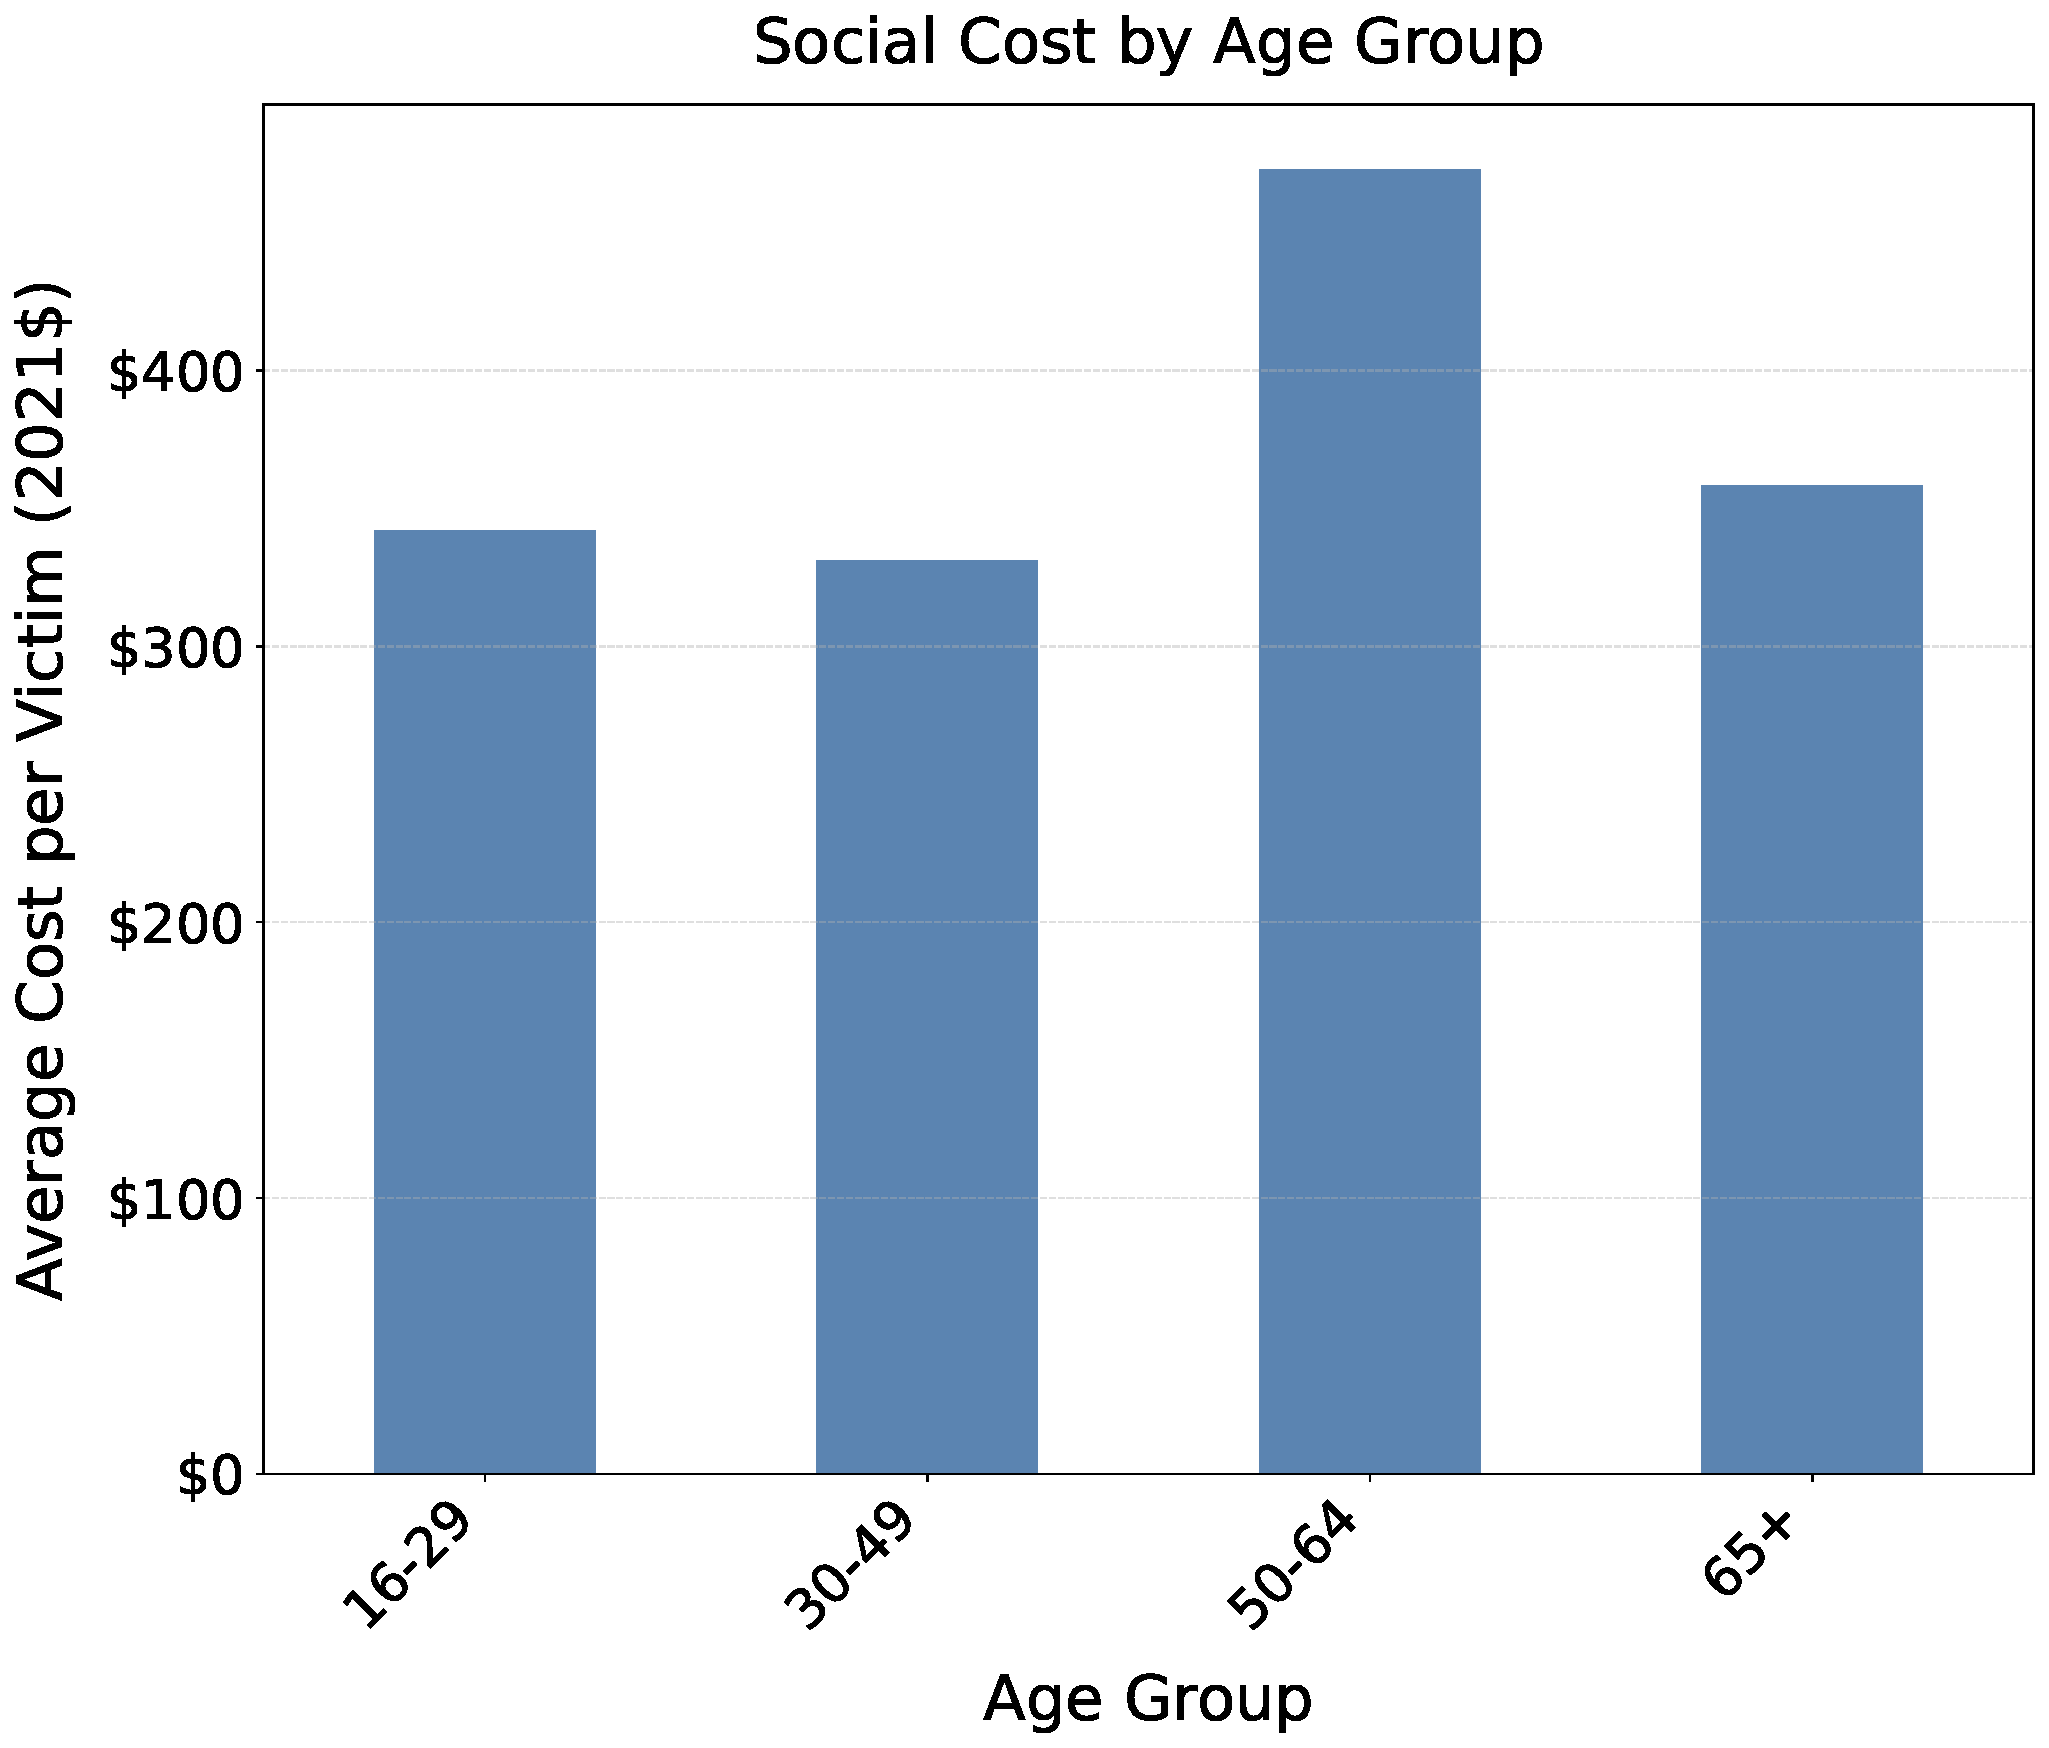
\includegraphics[width=\textwidth]{figures/social_cost/plot6_social_cost_by_age_group.pdf}
        \caption{By age group.}
        \label{fig:social_cost_age}
        
    \end{subfigure}
    \hfill % Adds horizontal space to push the images to the margins
    % --- Right Subfigure: Race/Ethnicity ---
    \begin{subfigure}[b]{0.48\textwidth}
        \centering
        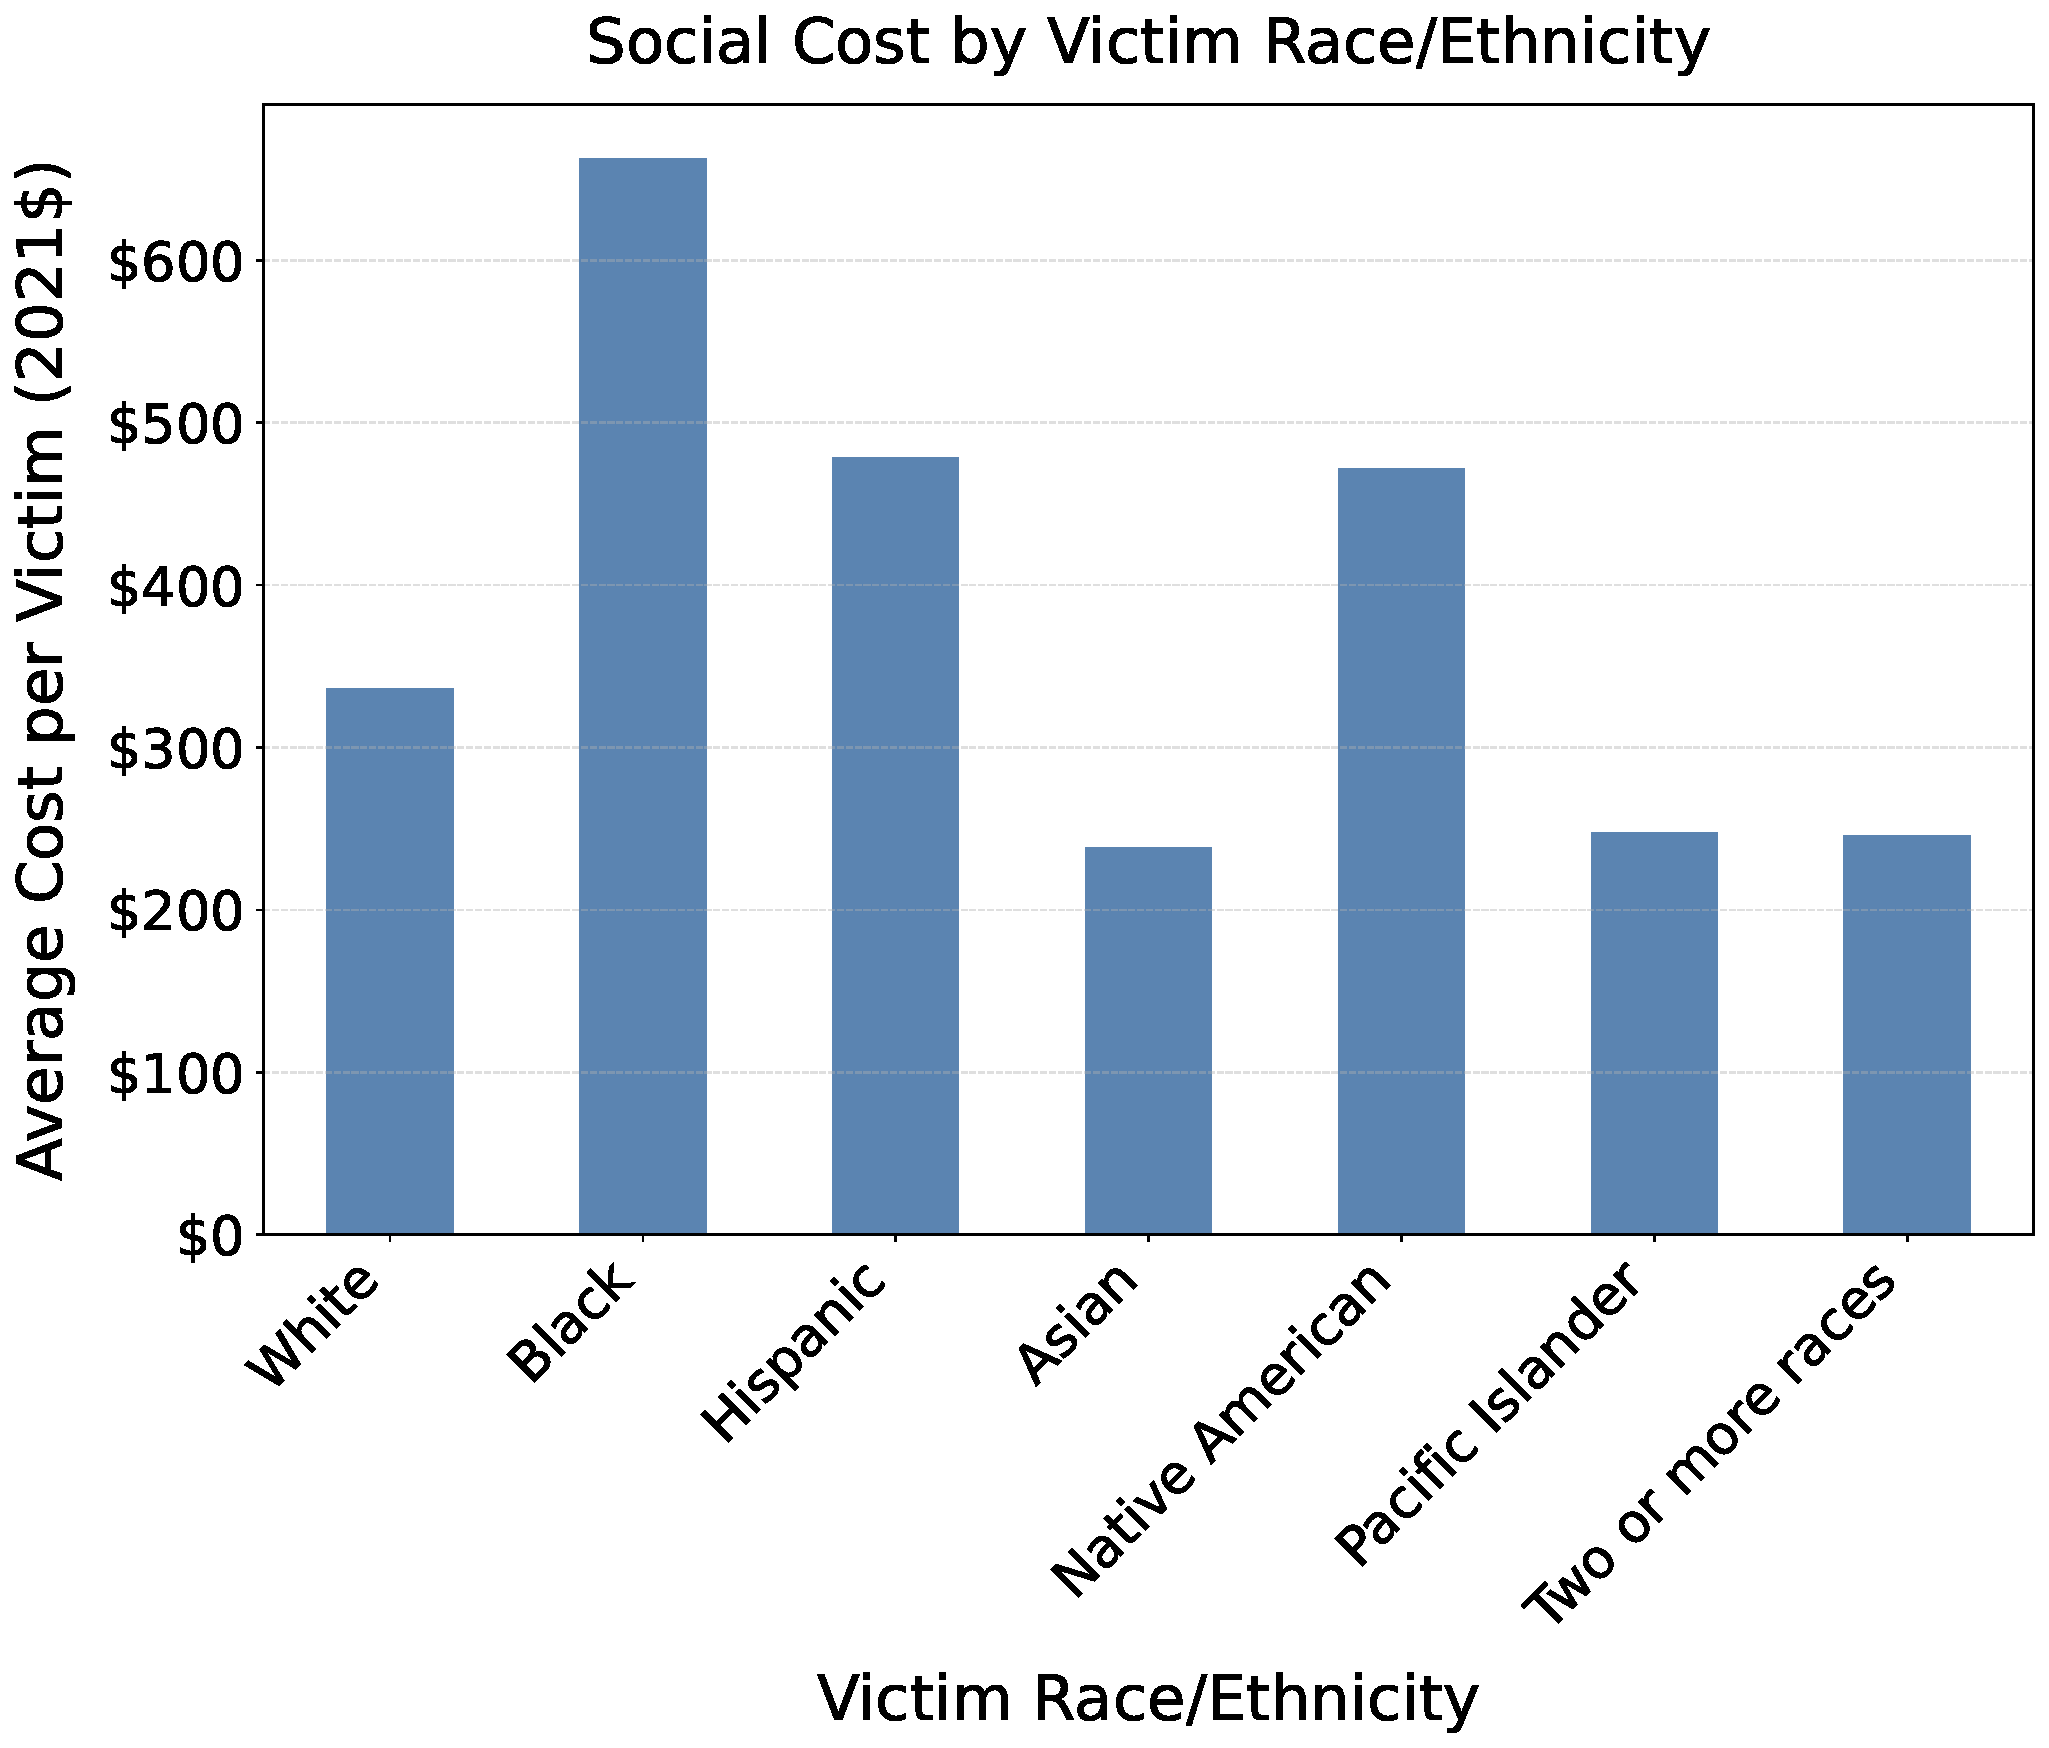
\includegraphics[width=\textwidth]{figures/social_cost/plot7_social_cost_by_victim_race_ethnicity.pdf}
        \caption{By race.}
        \label{fig:social_cost_race}
    \end{subfigure}
    
    \caption{Average social cost of data breaches by demographic characteristics (Age and Race).}
    \label{fig:social_cost_demographics}
\end{figure}

\begin{figure}[htbp]
    \centering
    % --- First Subfigure (Education) ---
    \begin{subfigure}[b]{0.48\textwidth}
        \centering
        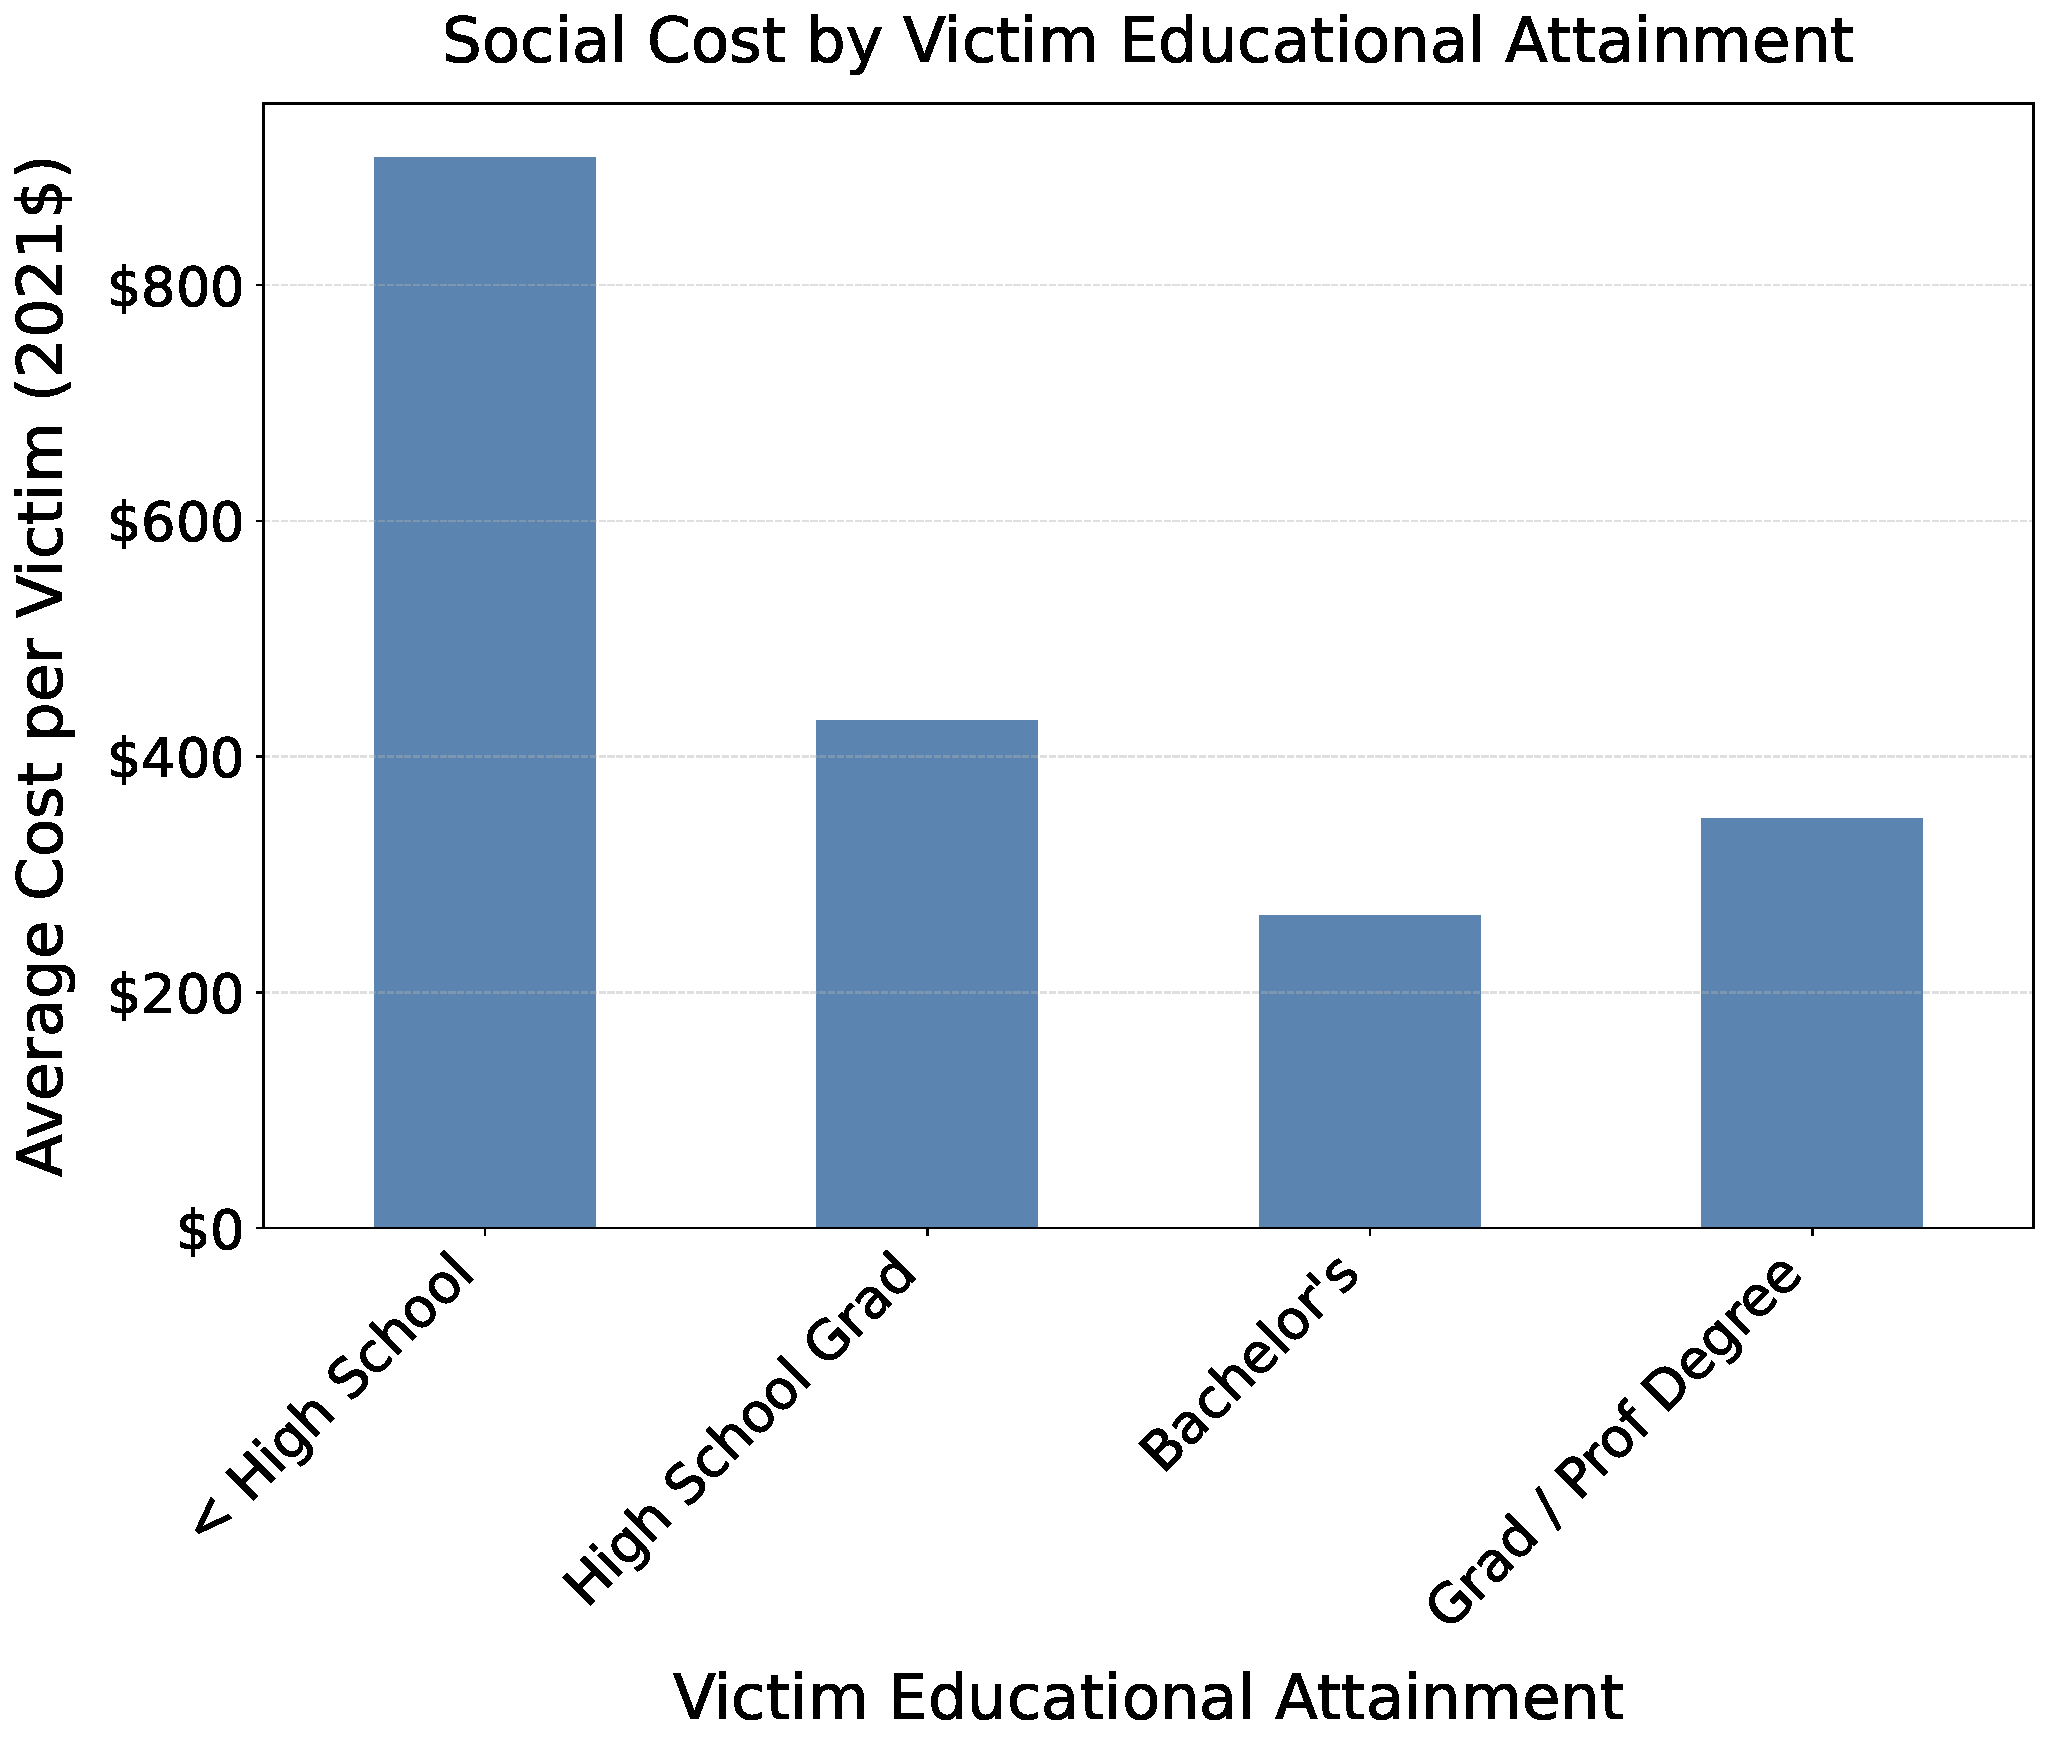
\includegraphics[width=\textwidth]{figures/social_cost/plot8_social_cost_by_victim_educational_attainment.pdf}
        \caption{By education.}
        \label{fig:social_cost_education}
    \end{subfigure}
    \hfill % Adds horizontal space between the two images
    % --- Second Subfigure (Income) ---
    \begin{subfigure}[b]{0.48\textwidth}
        \centering
        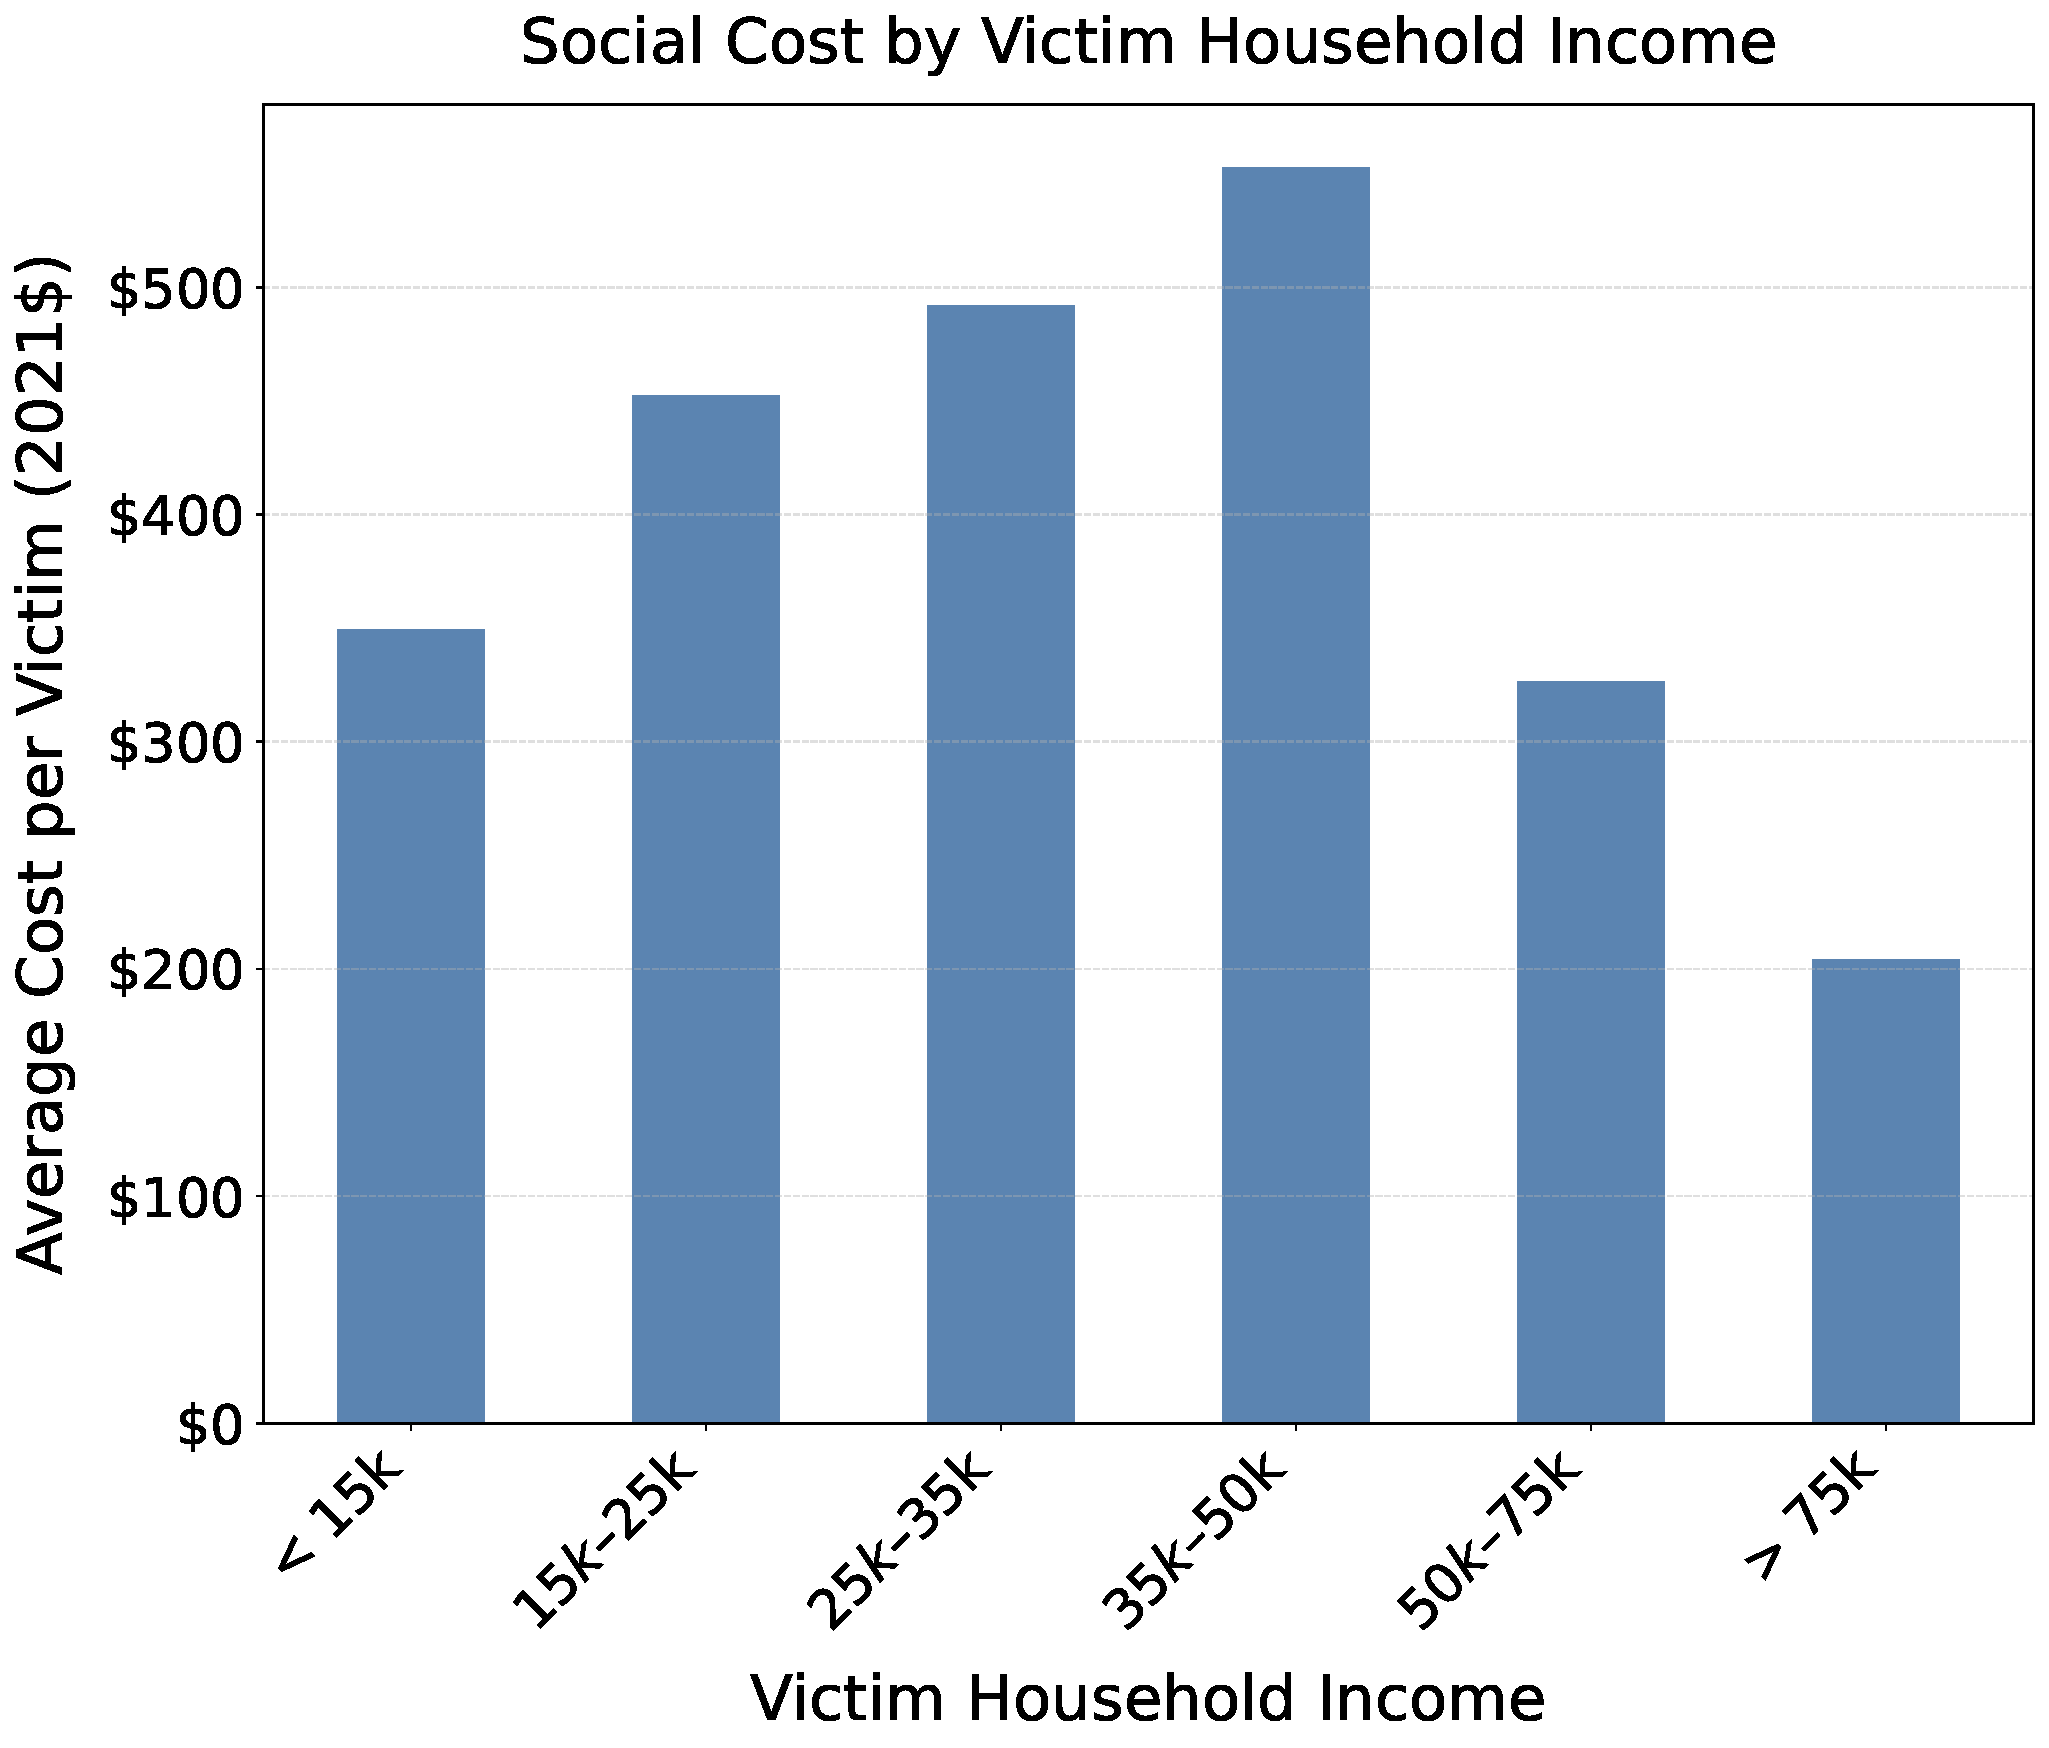
\includegraphics[width=\textwidth]{figures/social_cost/plot9_social_cost_by_victim_household_income.pdf}
        \caption{By income.}
        \label{fig:social_cost_income}
    \end{subfigure}
    
    \caption{Average social cost of data breaches segmented by demographic factors.}
    \label{fig:social_cost_combined}
\end{figure}

\section{Social Cost for Victims who were Notified of a Data Breach}
\label{app:social_cost_breach}




\subsection{Social Cost for Victims Notified that their Data was Breached}
\label{sec:breach_victim_social_cost}

While the overall social cost of IDT provides an interesting overview, the method by which a criminal obtains personal information can significantly influence the nature and severity of consequences for the victim. To investigate this, we compare victims who were notified that their data was leaked in a data breach to victims who were not notified of such (this was a question in the ITS survey). It is important to note that this distinction is only a proxy. The IDT of victims who were notified that their data was exposed could be attributed to the breach, but could also be just a coincidence (e.g. the data used for IDT was stolen separately). Our comparative analysis, detailed in Table \ref{tab:social_costs_by_type}, reveals an interesting trend, where victims who were notified of a data breach often incur lower per-victim social costs than those who were not. For example, in 2008, breach-notified victims faced a total social cost of \$428.72 per person, while victims not notified of a breach faced \$716.61. After 2016, the difference in social costs faced by breach-notified victims and victims not notified of a breach became much smaller, again likely as a result of the EMV shift as well as structural changes to the ITS survey. In 2021, breach-notified victims faced a total social cost of \$221.61 per person, while non-breach-notified victims faced \$222.64. These results could be due to the fact that breach victims are often alerted early by institutional safeguards, described in Section \ref{sec:incident_characteristics}, allowing for faster remediation. 

When considering the effect of social security number (SSN) compromise on the social cost, we found that SSN compromise was associated with higher social costs. As shown in Table \ref{tab:social_costs_ssn}, victims of an SSN breach consistently faced higher costs across nearly all cost categories compared to victims of a data breach whose SSNs were not leaked. In 2021, the per-victim social cost for an SSN-related breach victim was \$337.24, more than double the \$155.84 faced by victims whose SSN was not exposed. This difference is largely attributable to the lost time cost, since resolving an SSN requires more intensive interaction with government agencies and credit bureaus, leading to higher lost time costs and more emotional distress. Note that in Tables \ref{tab:social_costs_by_type} and \ref{tab:social_costs_ssn}, the breach victim numbers are relatively low compared to the hundreds of millions of users whose records have been exposed. This is because the vast majority of people whose records were exposed did not become IDT victims. 

% \com{You did not use this level of granularity of differentiated cost estimates in Sec 5 \& 6 when calculating the total, did you?}  \resp{No we didn't, I will move this to the appendix.}



\begin{table}[ht]
\centering
\caption{Social Costs of Identity Theft for Data Breach Victims versus Victims not Notified of a Breach.}
\label{tab:social_costs_by_type}

% Set up siunitx to handle the specific precision of your CSV data
\sisetup{
    group-separator={,}, 
    group-minimum-digits=4,
    round-mode=places,
    round-precision=2 % Rounds decimals to 2 places for readability while keeping raw data in code
}

\footnotesize 

\begin{tabular}{
  l l 
  S[table-format=8.2] % Total Weighted Victims
  S[table-format=3.2] % Avg. Out-of-Pocket Loss
  S[table-format=1.2] % Avg. Legal Cost
  S[table-format=3.2] % Avg. Lost Time Cost
  S[table-format=1.2] % Avg. Healthcare Cost
  S[table-format=4.2] % Total Social Cost per Victim
  S[table-format=11.2] % Total National Social Cost
}
\toprule
{\thead{Year}} & {\thead{Group}} & {\thead{Total \\ Weighted \\ Victims}} & {\thead{Avg. Out-of- \\ Pocket Loss (\$)}} & {\thead{Avg. \\ Legal \\ Cost (\$)}} & {\thead{Avg. Lost \\ Time \\ Cost (\$)}} & {\thead{Avg. \\ Healthcare \\ Cost (\$)}} & {\thead{Total Social \\ Cost per \\ Victim (\$)}} & {\thead{Total \\ National \\ Social Cost (\$)}} \\
\midrule

\multirow{2}{*}{\textbf{2008}} & Breach & 1607267.02 & 151.84 & 6.38 & 268.50 & 2.01 & 428.72 & 689074940.96 \\
& Non-Breach & 9884125.17 & 494.79 & 5.64 & 215.17 & 1.01 & 716.61 & 7083094274.71 \\
\midrule

\multirow{2}{*}{\textbf{2012}} & Breach & 2108805.36 & 62.79 & 1.58 & 162.33 & 1.21 & 227.91 & 480627748.03 \\
& Non-Breach & 14298624.65 & 510.84 & 4.06 & 233.81 & 0.93 & 749.63 & 10718748301.44 \\
\midrule

\multirow{2}{*}{\textbf{2014}} & Breach & 3511656.24 & 953.50 & 2.28 & 206.12 & 0.90 & 1162.80 & 4083351744.90 \\
& Non-Breach & 13941551.04 & 291.84 & 3.60 & 169.56 & 0.63 & 465.63 & 6491616163.16 \\
\midrule

\multirow{2}{*}{\textbf{2016}} & Breach & 5426070.22 & 79.43 & 3.59 & 135.56 & 0.73 & 219.31 & 1190005853.99 \\
& Non-Breach & 19851764.64 & 78.57 & 3.16 & 116.15 & 0.65 & 198.52 & 3941058367.52 \\
\midrule

\multirow{2}{*}{\textbf{2018}} & Breach & 6432045.33 & 69.51 & 0.44 & 127.64 & 0.83 & 198.43 & 1276280960.88 \\
& Non-Breach & 15869463.46 & 85.00 & 1.67 & 118.13 & 0.52 & 205.32 & 3258310823.36 \\
\midrule

\multirow{2}{*}{\textbf{2021}} & Breach & 5747212.66 & 79.33 & 1.82 & 139.16 & 1.30 & 221.61 & 1273655029.05 \\
& Non-Breach & 17868922.65 & 90.67 & 1.78 & 129.54 & 0.66 & 222.64 & 3978280747.92 \\
\bottomrule
\end{tabular}
\end{table}

\begin{table}[ht]
\centering
\caption{Social Costs of Identity Theft for Breach Victims by SSN Breach Status and Year.}
\label{tab:social_costs_ssn}

% siunitx setup to handle CSV precision and comma separation
\sisetup{
    group-separator={,}, 
    group-minimum-digits=4,
    round-mode=places,
    round-precision=2
}

\footnotesize 

\begin{tabular}{
  l l 
  S[table-format=7.2] % Total Weighted Victims
  S[table-format=4.2] % Avg. Out-of-Pocket Loss
  S[table-format=1.2] % Avg. Legal Cost
  S[table-format=3.2] % Avg. Lost Time Cost
  S[table-format=1.2] % Avg. Healthcare Cost
  S[table-format=4.2] % Total Social Cost per Victim
  S[table-format=10.2] % Total National Social Cost
}
\toprule
{\thead{Year}} & {\thead{Group}} & {\thead{Total \\ Weighted \\ Victims}} & {\thead{Avg. Out-of- \\ Pocket Loss (\$)}} & {\thead{Avg. \\ Legal \\ Cost (\$)}} & {\thead{Avg. Lost \\ Time \\ Cost (\$)}} & {\thead{Avg. \\ Healthcare \\ Cost (\$)}} & {\thead{Total Social \\ Cost per \\ Victim (\$)}} & {\thead{Total \\ National \\ Social Cost (\$)}} \\
\midrule

\multirow{2}{*}{\textbf{2008}} & SSN Exposed & 770793.01 & 215.16 & 6.55 & 434.98 & 2.48 & 659.18 & 508087860.87 \\
& SSN Not Exposed & 693362.57 & 32.22 & 2.98 & 119.82 & 1.90 & 156.93 & 108810349.32 \\
\midrule

\multirow{2}{*}{\textbf{2012}} & SSN Exposed & 707503.97 & 62.25 & 2.87 & 260.87 & 1.79 & 327.77 & 231897760.95 \\
& SSN Not Exposed & 1299621.39 & 65.07 & 1.01 & 112.66 & 0.65 & 179.40 & 233150967.13 \\
\midrule

\multirow{2}{*}{\textbf{2014}} & SSN Exposed & 548160.54 & 2547.90 & 2.46 & 453.16 & 3.49 & 3007.00 & 1648321393.54 \\
& SSN Not Exposed & 2818797.89 & 690.37 & 2.36 & 164.17 & 0.44 & 857.35 & 2416687892.50 \\
\midrule

\multirow{2}{*}{\textbf{2016}} & SSN Exposed & 2635897.53 & 101.19 & 5.54 & 165.78 & 1.11 & 273.62 & 721247422.80 \\
& SSN Not Exposed & 2400462.74 & 64.46 & 2.04 & 115.06 & 0.44 & 181.99 & 436868321.44 \\
\midrule

\multirow{2}{*}{\textbf{2018}} & SSN Exposed & 1345760.50 & 62.70 & 0.65 & 174.79 & 1.44 & 239.57 & 322404919.80 \\
& SSN Not Exposed & 1425157.50 & 70.06 & 0.00 & 118.03 & 0.37 & 188.46 & 268591628.42 \\
\midrule

\multirow{2}{*}{\textbf{2021}} & SSN Exposed & 1177409.42 & 137.56 & 4.58 & 193.08 & 2.02 & 337.24 & 397069893.06 \\
& SSN Not Exposed & 1422882.78 & 37.73 & 0.99 & 116.04 & 1.09 & 155.84 & 221742562.24 \\
\bottomrule
\end{tabular}
\end{table}


% \section{Imputation of Undisclosed Records}
% \label{app:imputation_nu}

% To ensure the continuity of the data breach chronology, we addressed the volume of incidents lacking disclosed record counts by calculating an annual baseline number of undisclosed records, $n_u$. 




\section{Inflation Adjustments}
\label{app:inflation}
The formula used to convert a nominal monetary value from a given year to its real value in 2021 dollars is as follows:
\begin{equation}
\label{eq:inflation_adjustment}
\text{Adjusted Value (in 2021 \$)} = \text{Nominal Value} \times \left( \frac{\text{CPI}_{2021}}{\text{CPI}_{\text{Original Year}}} \right)
\end{equation}

Table \ref{tab:appendix_cpi} displays all the CPI values that were used for these calculations. This inflation adjustment was applied to any monetary value in this paper. These CPI values were obtained from the U.S. Bureau of Labor Statistics \cite{BLS_CPI, USInflationCalc_CPI}.

\begin{table}[ht]
\centering
\caption{Annual Average Consumer Price Index (CPI)}
\label{tab:appendix_cpi}
\begin{tabular}{lr}
\toprule
\textbf{Year} & \textbf{Annual Average CPI} \\
\midrule
2008 & 215.297 \\
2012 & 233.165 \\
2014 & 236.736 \\
2016 & 240.007 \\
2018 & 251.107 \\
2021 & 270.970 \\
% 2023 & 304.702 \\
% 2024 & 313.689 \\
\bottomrule
\end{tabular}
\end{table}

\section{Average Private Nonfarm Hourly Wages}
\label{app:hourly_wages}
To estimate opportunity cost of lost time in the social cost calculations, time lost was multiplied by the respective year's average hourly wage, shown in Table \ref{tab:appendix_wage}. This private nonfarm hourly wage data represents the vast majority of the U.S. workforce, and was obtained from \cite{FRED_Wage}.

\begin{table}[ht]
\centering
\caption{Nominal and Inflation-Adjusted Average Private Hourly Wage}
\label{tab:appendix_wage}
\begin{tabular}{lrr}
\toprule
\textbf{Year} & \multicolumn{2}{c}{\textbf{Average Private Hourly Wage}} \\
\cmidrule(lr){2-3} % Draws a line under columns 2 and 3 only
& \textbf{Nominal} & \textbf{Adjusted} \\
\midrule
2008 & 21.19 & 26.67 \\
2012 & 23.26 & 27.03 \\
2014 & 24.23 & 27.73 \\
2016 & 25.37 & 28.64 \\
2018 & 26.72 & 28.83 \\
2021 & 29.92 & 29.92 \\
\bottomrule
\end{tabular}
\end{table}

\section{Fixed Service Costs for Social Cost Calculations}
\label{app:fixed_service_costs}
To estimate the cost of hiring a lawyer, a doctor or therapy appointment, or obtaining medication, we constructed the following Table \ref{tab:appendix_cost_estimates_sourced}, where costs were also adjusted for inflation.

\begin{table}[ht]
\centering
\caption{Cost Estimates and Sources for Social Cost Calculations}
\label{tab:appendix_cost_estimates_sourced}
\small % Using a smaller font size to help the table fit
\begin{tabular}{l l r c r l l}
\toprule
\thead{Item} & 
\thead{Reported \\ Nominal Cost} & 
\thead{Assumed \\ Nominal \\ Cost (\$)} & 
\thead{Source \\ Year} & 
\thead{Adjusted \\ Cost \\ (2021 \$)} & 
\thead{Notes} &
\thead{Source} \\
\midrule
Lawyer & \$327 per hour & 500 & 2023 & 444.65 & Based on approx. 1.5 hours & \cite{USNews_Lawyer}\\
Doctor Visit & \$79--172 & 100 & 2024 & 86.38 & Without insurance & \cite{DebtOrg_Doctor} \\
Therapist Visit & \$100--200 & 100 & 2024 & 86.38 & Without insurance & \cite{GoodRx_Therapy} \\
Medication & \$50 & 50 & 2018 & 53.96 & Generic prescription & \cite{CBO_Prescription} \\
\bottomrule
\end{tabular}
\end{table}

% \section{Data Breach Chronology Data Supplementation}
% \label{app:PRC_data}

% The number of records exposed for major breaches were referenced as detailed in Table \ref{tab:major_breaches}. The cross-referencing of the PRC, Maine, and New Hampshire datasets was performed using fuzzy string matching in Python. Matches between the state-level predictor and national baseline were only accepted if they met a token sort ratio of 0.7 or higher. To further ensure data integrity, a manual audit was done on the high-magnitude matches to prevent pairing of distinct entities with similar names. The magnitude estimation was performed using Ordinary Least Squares (OLS) regression. 

% The resulting multiplier represents the scaling factor between a localized sample and the estimated national impact. 


% \begin{table}[ht]
% \centering
% \caption{Major Breach Events and Sources.}
% \label{tab:major_breaches}
% \begin{tabular}{@{}llrl@{}}
% \toprule
% \textbf{Entity / Event} & \textbf{Month/Year} & \textbf{Records Exposed} & \textbf{Source} \\ \midrule
% Bank of New York Mellon & May 2008 & 12,500,000 & \cite{Reuters_BNY_Mellon} \\
% Heartland Payment Systems & Jan 2009 & 130,000,000 & \cite{USCourts_Heartland} \\
% Sony PlayStation Network & Apr 2011 & 77,000,000 & \cite{OAIC_Sony} \\
% Target Corporation & Dec 2013 & 40,000,000 & \cite{Target_Breach} \\
% Home Depot & Sep 2014 & 56,000,000 & \cite{HomeDepot_Breach} \\
% Equifax & Sep 2017 & 147,000,000 & \cite{House_Equifax} \\ \bottomrule
% \end{tabular}
% \end{table}



% Results of the OLS regression are detailed in Table \ref{tab:regression_stats} below.

% \begin{table}[h]
% \centering
% \caption{OLS Regression Results for National Magnitude Estimation ($N=606$)}
% \label{tab:regression_stats}
% \begin{tabular}{l S[table-format=3.4]} % Aligns decimals, allows 3 digits before and 4 after
% \toprule
% \textbf{Metric} & {\textbf{Value}} \\ 
% \midrule
% Multiplier           & 153.22   \\
% Standard Error (SE)            & 16.49    \\
% \addlinespace % Adds a small gap for readability
% 95\% Conf. Interval (Low)      & 120.91   \\
% 95\% Conf. Interval (High)     & 185.54   \\ 
% \bottomrule
% \end{tabular}
% \end{table}






\section{Details of Dataset Filtering}

% \subsection{Dataset Filtering}

To create the sample of identity theft victims, the dataset was filtered to include any respondent who answered "Yes" (coded as 1) to any of the following five questions concerning events in the past 12 months: misuse of an existing bank account, misuse of an existing credit card, misuse of another existing account, fraudulent opening of a new account, or the use of personal information for other fraudulent purposes. This is detailed in Table \ref{tab:victim_filtering}.

\begin{table}[ht]
\centering
\caption{Filtering Rules to Identify Identity Theft Victims}
\label{tab:victim_filtering}
\begin{tabular}{p{0.6\textwidth}l}
\toprule
\textbf{Condition Met if Variable...} & \textbf{Equals Value...} \\
\midrule
\multicolumn{2}{l}{\textit{A respondent is a victim if ANY of the following are true:}} \\
\addlinespace % Adds a bit of vertical space
EXISTING\_BANK\_ACCT\_MISUSE\_12MO   & 1 (Yes) \\
EXISTING\_CC\_MISUSE\_12MO         & 1 (Yes) \\
EXISTING\_OTHER\_ACCT\_MISUSE\_12MO  & 1 (Yes) \\
NEW\_ACCT\_OPENED\_12MO            & 1 (Yes) \\
OTHER\_FRAUDULENT\_PURPOSE\_12MO   & 1 (Yes) \\
\bottomrule
\end{tabular}
\end{table}

After identifying all identity theft victims (both attempted and successful), a second filtering step was applied to remove records where the theft was attempted but not successful. The specific variables and codes used to identify an "attempted only" case vary by survey year due to changes in the survey instrument. For the 2021 survey, no filtering was necessary, as the questionnaire was designed to capture only successful incidents. The precise logic for each year is detailed in Table \ref{tab:successful_theft_filtering}.

\begin{table}[ht]
\centering
\caption{Rules for Identifying and Removing 'Attempted Only' Identity Theft Incidents}
\vspace{0.2cm}
\label{tab:successful_theft_filtering}
\begin{tabular}{lp{0.65\textwidth}}
\toprule
\textbf{Survey Year} & \textbf{Condition to REMOVE a record because theft was not successful} \\
\midrule
\addlinespace % Adds a bit of vertical space
2008 & A record is removed if \texttt{VS012=2} AND \texttt{VS014=2} AND \texttt{VS016=2} AND \texttt{VS018=2} AND \texttt{VS020=2}. \\
\addlinespace
2012 & A record is removed if the variable \texttt{VS098 = 009} (Not applicable, it was not actually used). \\
\addlinespace
2014 & A record is removed if the variable \texttt{VS093 = 009}  (Not applicable, it was not actually used). \\
\addlinespace
2016 & A record is removed if the variable \texttt{VS093 = 9}  (Not applicable, it was not actually misused). \\
\addlinespace
2018 & A record is removed if the variable \texttt{VS093 = 9}  (Not applicable, it was not actually misused). \\
\addlinespace
2021 & No filtering action is needed. The survey design for this year ensures all identified victims are successful incidents. \\
\bottomrule
\end{tabular}
\end{table}

\section{ITS Victim Timeline}
\label{app:timeline}
To plot the number of reported identity thefts per month from the ITS dataset, the following assumptions were made. The primary variable used for the timeline is the month in which the victim first discovered the identity theft. For survey years where this specific "discovery month" was explicitly recorded (such as the redesigned 2021 ITS), that value was used directly. For survey waves or individual records where a specific discovery month was missing or not collected, the month was estimated using the Interview Quarter variable. In cases where only the interview quarter was available, incidents were mapped to the mid-month of that quarter to provide a representative point estimate (e.g., Quarter 1 $\rightarrow$ February, Quarter 2 $\rightarrow$ May, Quarter 3 $\rightarrow$ August, Quarter 4 $\rightarrow$ November). This ensures the timeline reflects the general seasonal distribution of reports while acknowledging the six-month reference period typically used in the NCVS core interview. Monthly counts were calculated by summing the final ITS weights of all confirmed victims discovered or reported in that month. This allows the timeline to represent national-level estimates of identity theft discovery rather than raw sample counts. 

\section{Dynamic Saturation Model}
\label{app:sat_model}
Here we display the month-to-month overlay and conversion rate results, as well as Wilcoxon signed-rank testing results, for the output of our dynamic saturation model (with $Y=1$)(proposed in Section \ref{sec:estimating_number_records}). Recall that the purpose of this model is to take the augmented PRC data as an input, and output the estimated number of unique individuals whose data was compromised.

\begin{figure}[htbp]
    \centering
    % First Figure
    \begin{minipage}[t]{0.32\textwidth}
        \centering
        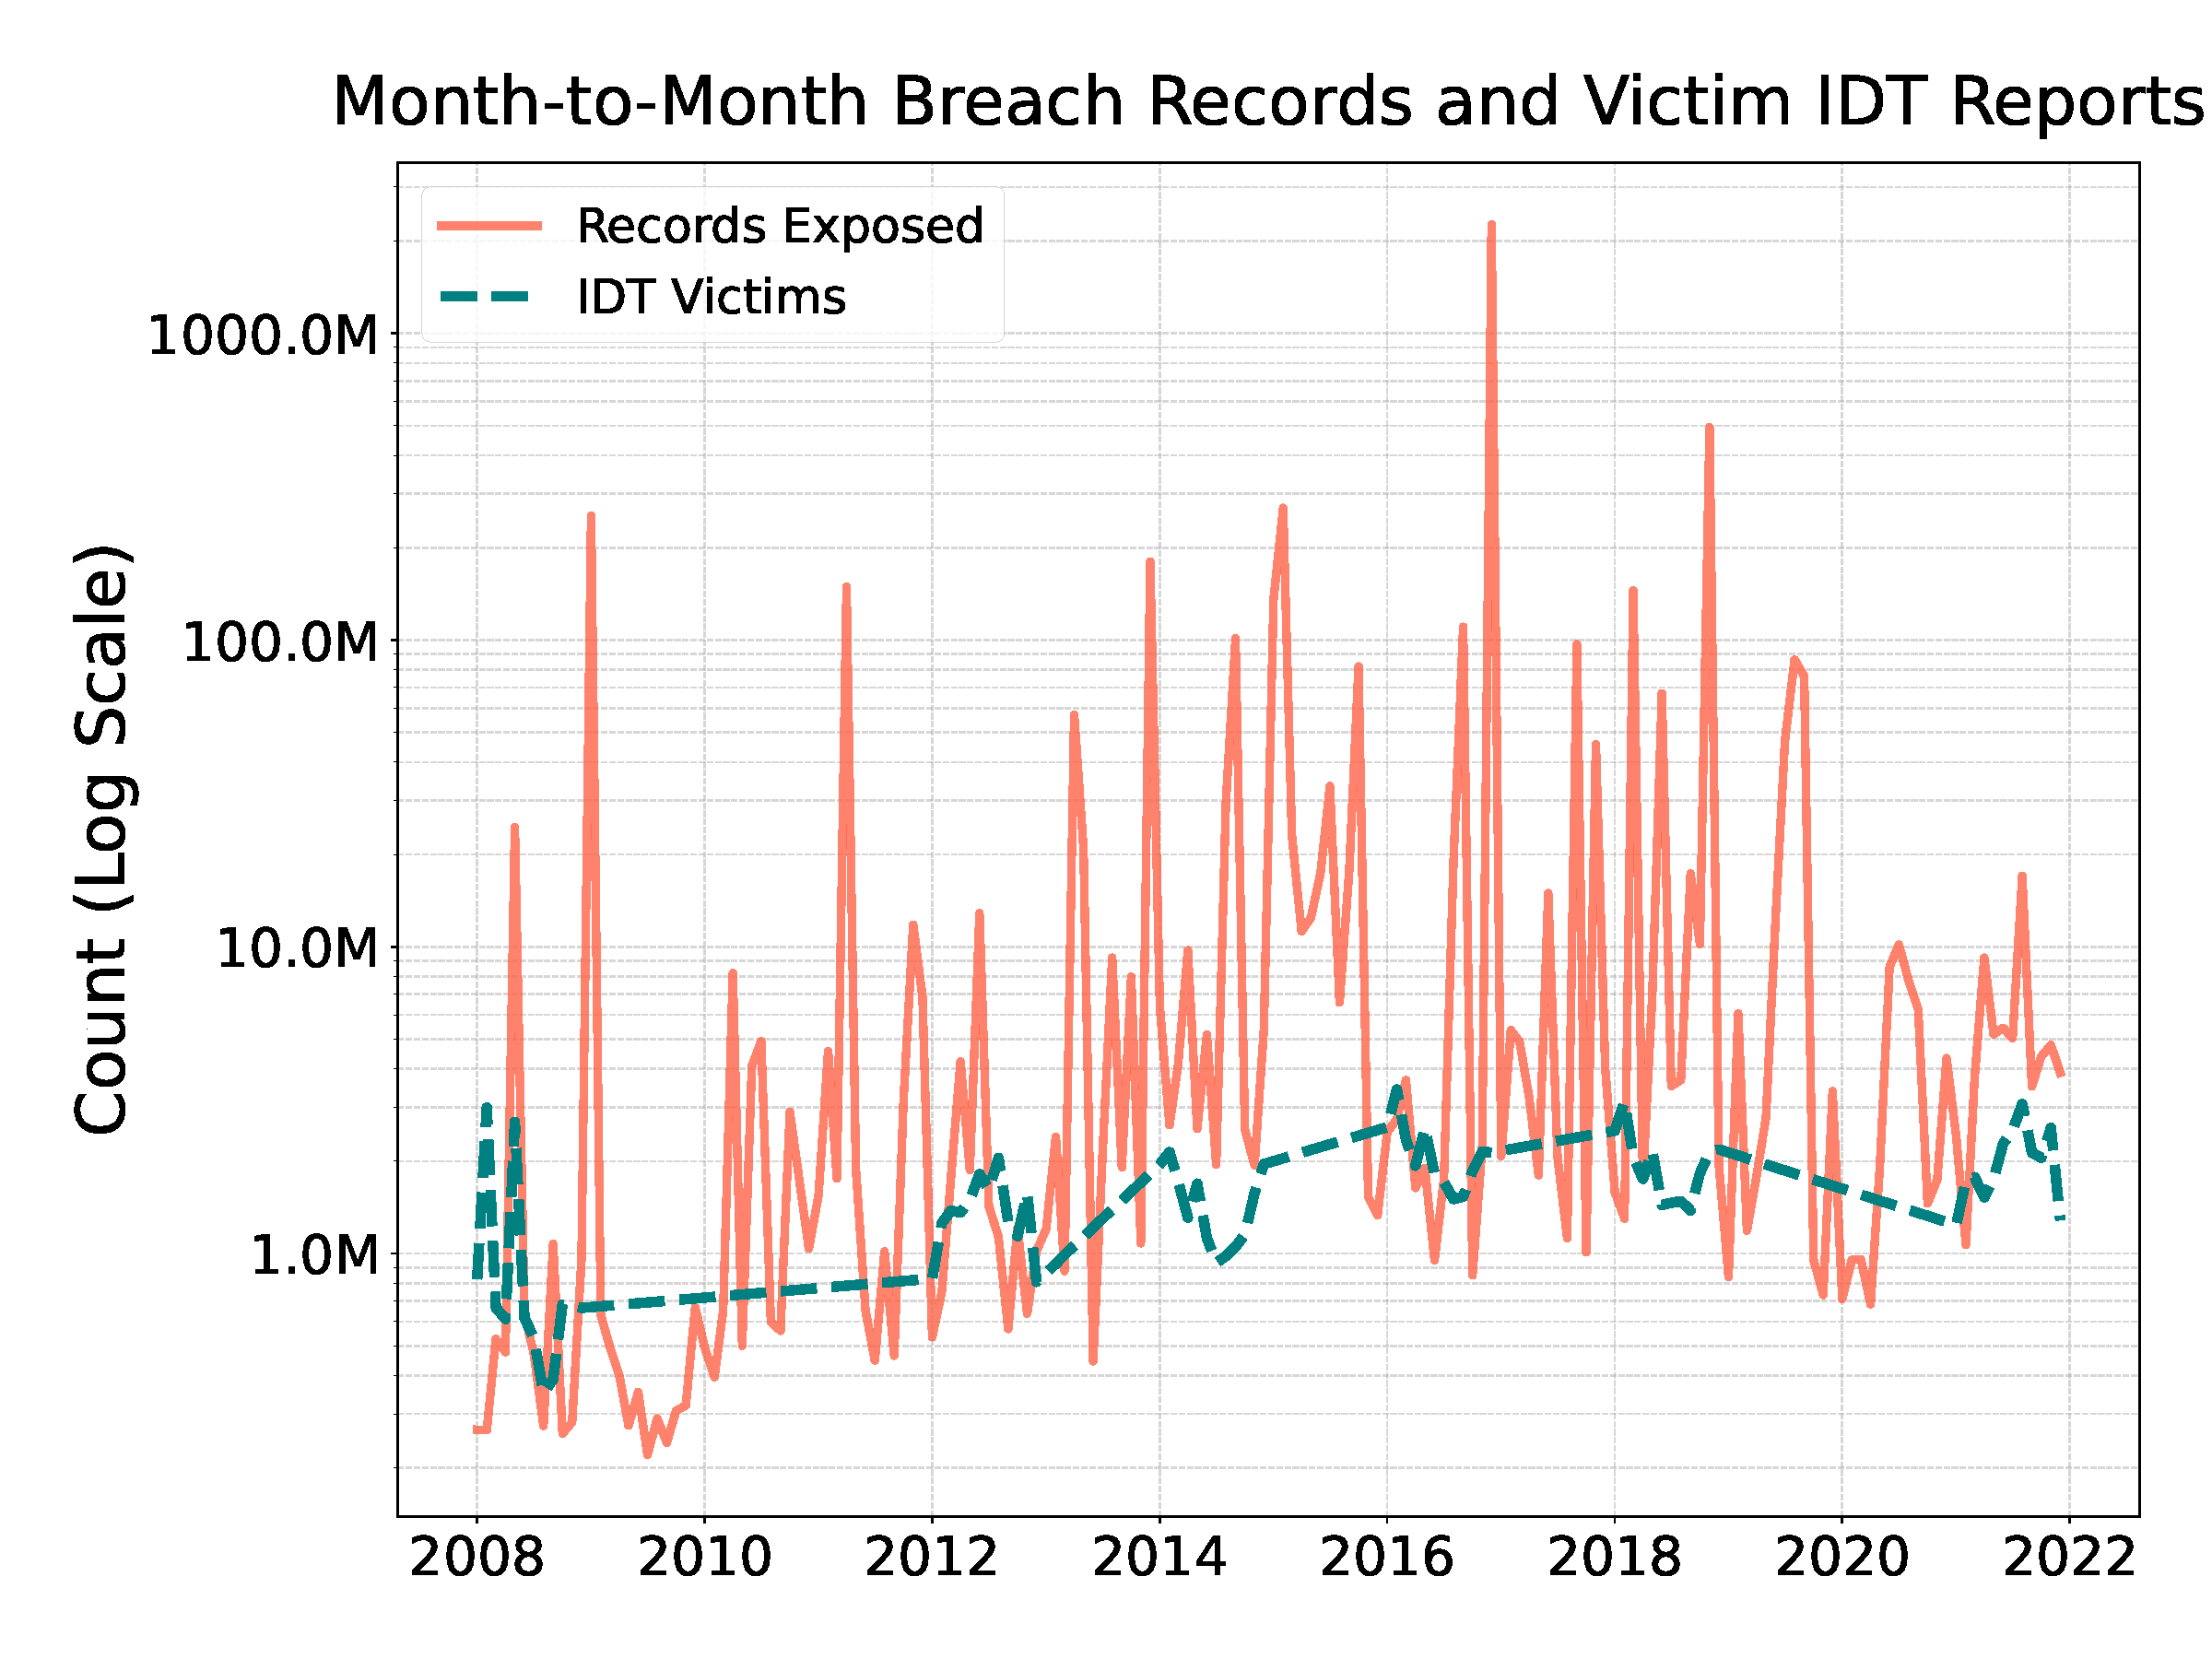
\includegraphics[width=\textwidth]{figures/part5/overlay.pdf}
        \caption{Estimated number of unique individuals compromised (saturation model PRC)} and number of reported IDT victims (ITS).
        \label{fig:saturation_fig5}
    \end{minipage}
    \hfill 
    % Second Figure
    \begin{minipage}[t]{0.32\textwidth}
        \centering
        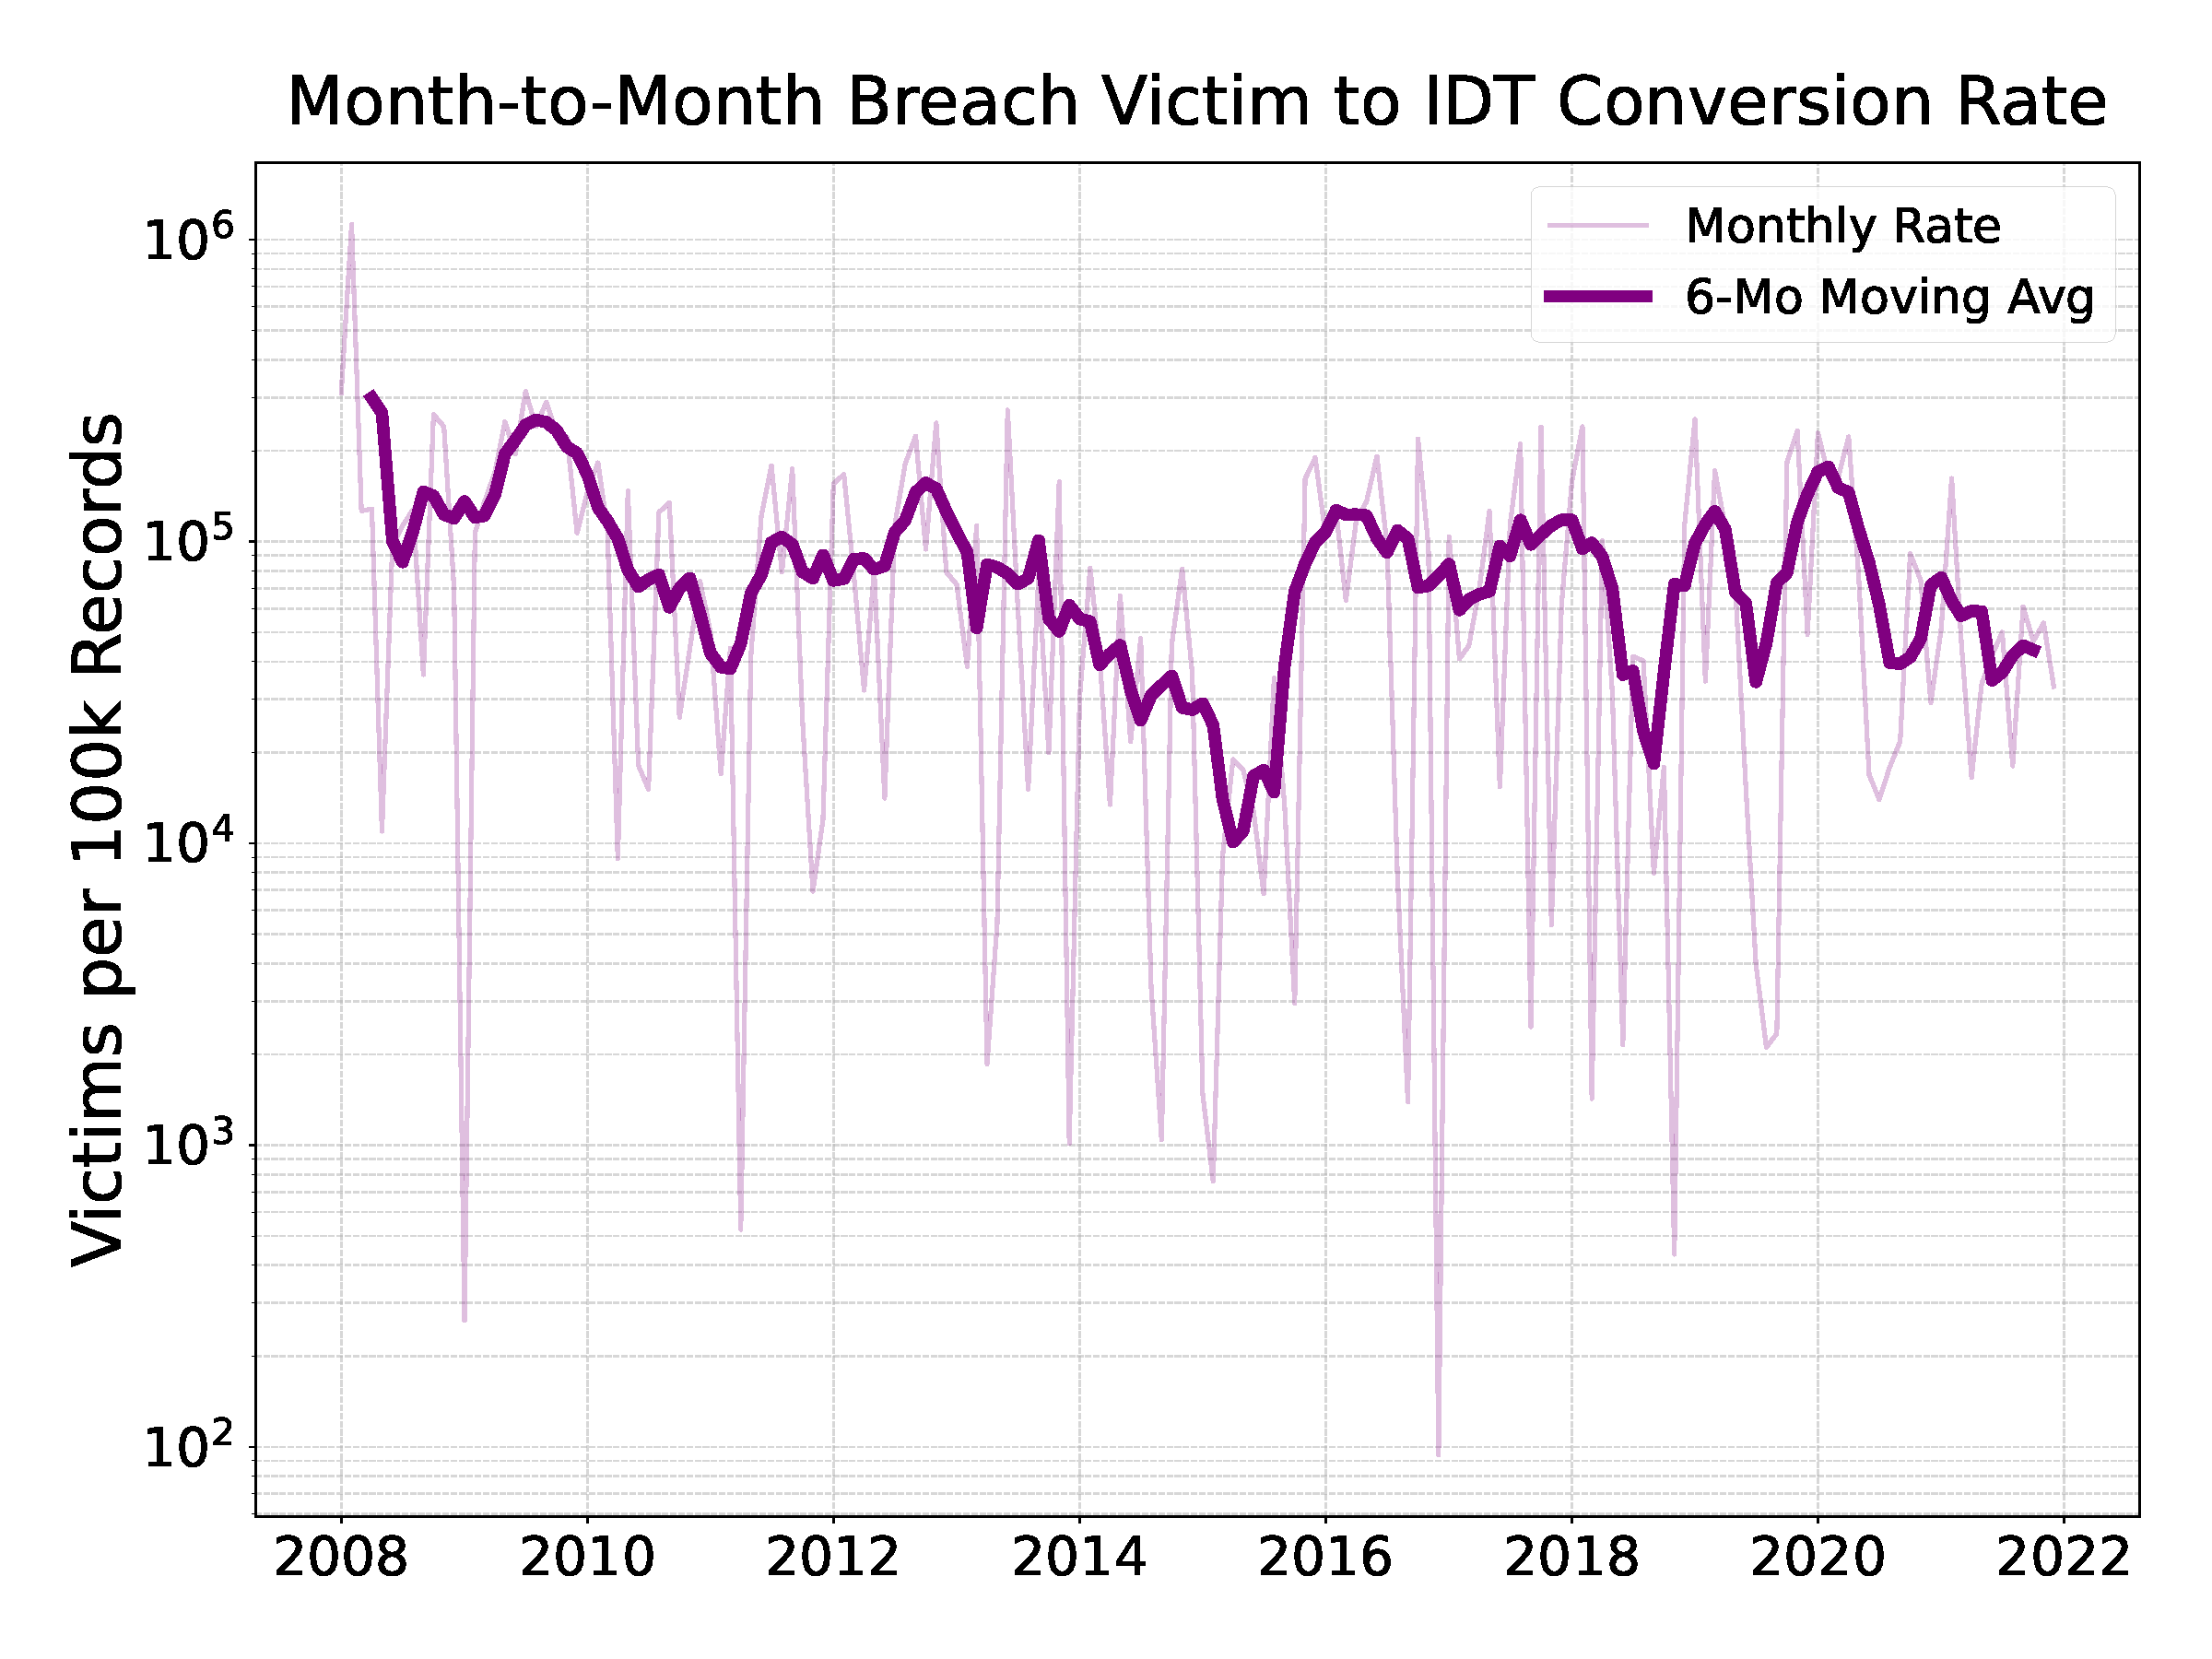
\includegraphics[width=\textwidth]{figures/part5/conversion_rate.pdf}
        \caption{Saturation model conversion rates from data being breached to becoming an IDT victim.}
        \label{fig:saturation_conversion_rate}
    \end{minipage}
    \hfill
    % Third Figure
    \begin{minipage}[t]{0.32\textwidth}
        \centering
        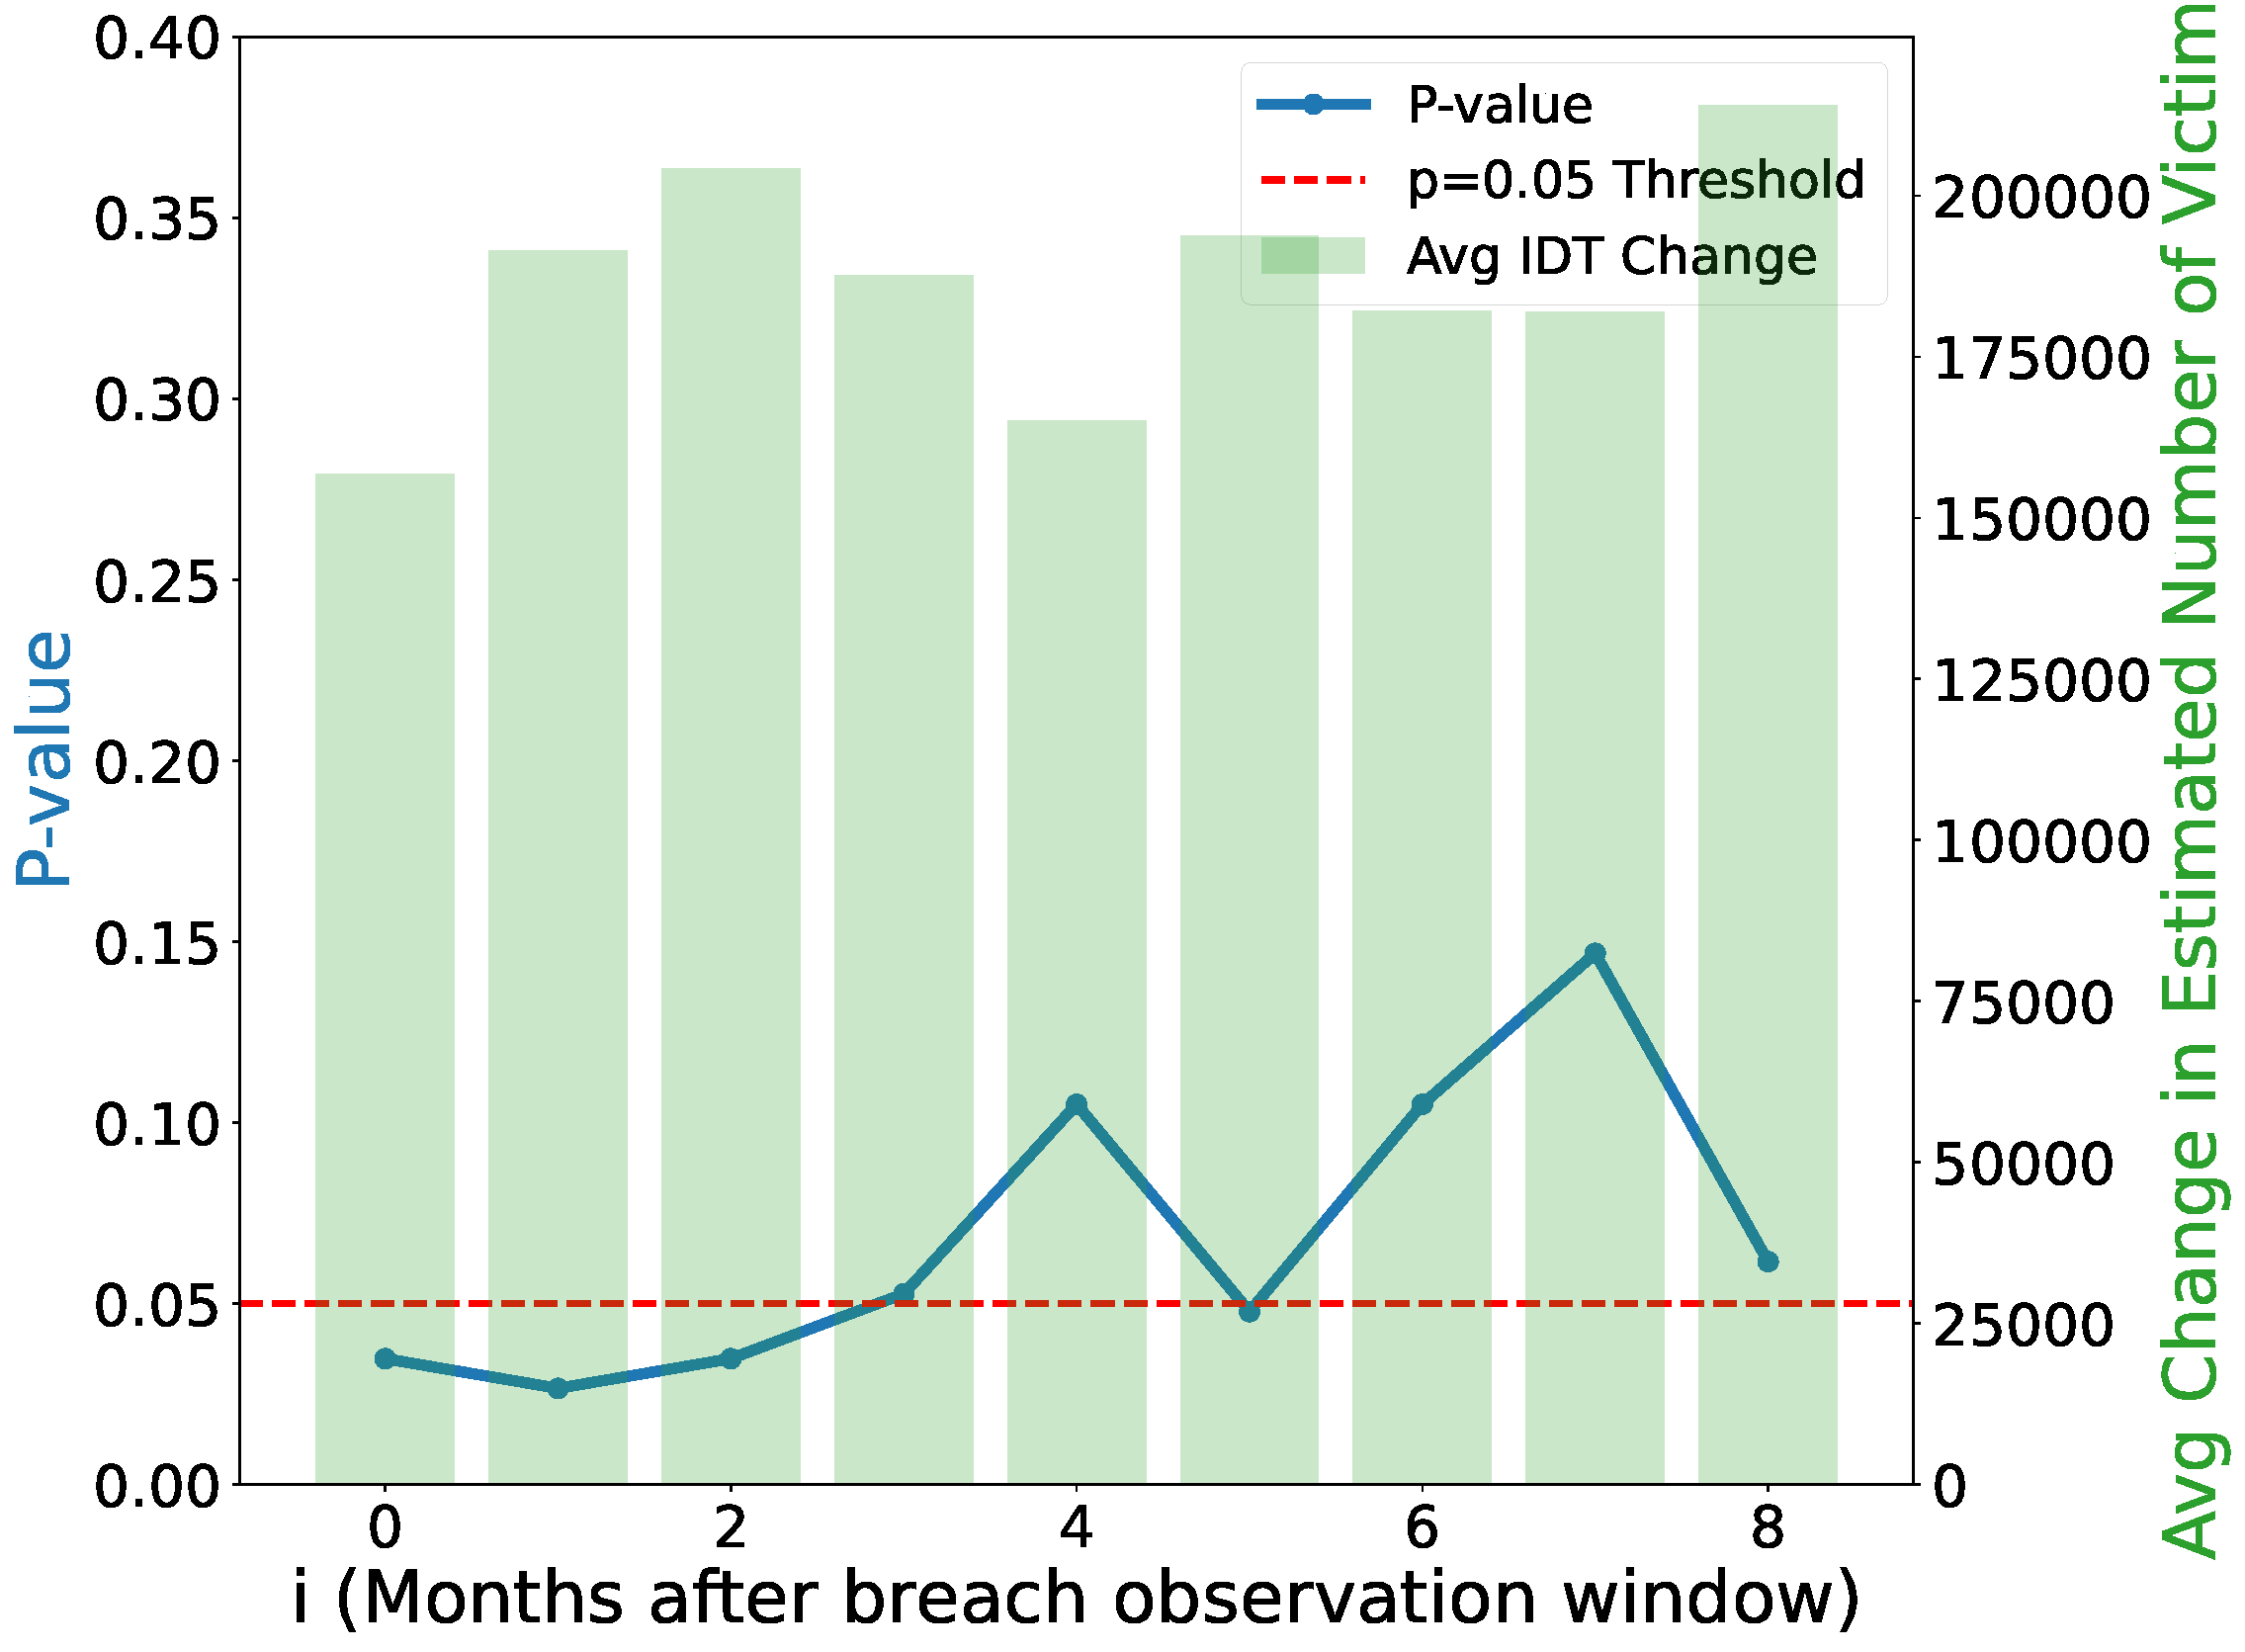
\includegraphics[width=\textwidth]{figures/part6/longitudinal_sweep_saturation_model.pdf}
        \caption{Wilcoxon signed-rank test results for the saturation model PRC data breach chronology data.}
        \label{fig:wilcoxon_sat}
    \end{minipage}
\end{figure}

\section{Harmonization Codes}
\label{app: dataset_harmonization}

The following new variables were created according to the mappings below in order to harmonize similar variables from different years of datasets.

\begin{table}[ht]
\centering
\caption{Harmonization Map for EXISTING\_BANK\_ACCT\_MISUSE\_12MO}
\label{tab:bank_misuse_codes}
\begin{tabular}{llll}
\toprule
\textbf{Year} & \textbf{Variable Name} & \textbf{Yes Code} & \textbf{No Code} \\
\midrule
2008 & \texttt{VS013} & 1  & 2  \\
2012 & \texttt{VS012} & 01 & 02 \\
2014 & \texttt{VS012} & 01 & 02 \\
2016 & \texttt{VS012} & 1  & 2  \\
2018 & \texttt{VS012} & 1  & 2  \\
2021 & \texttt{VS012} & 1  & 2  \\
\bottomrule
\end{tabular}
\end{table}


\begin{table}[ht]
\centering
\caption{Harmonization Map for EXISTING\_CC\_MISUSE\_12MO}
\label{tab:cc_misuse_codes}
\begin{tabular}{llll}
\toprule
\textbf{Year} & \textbf{Variable Name} & \textbf{Yes Code} & \textbf{No Code} \\
\midrule
2008 & \texttt{VS011} & 1  & 2  \\
2012 & \texttt{VS016} & 01 & 02 \\
2014 & \texttt{VS017} & 01 & 02 \\
2016 & \texttt{VS017} & 1  & 2  \\
2018 & \texttt{VS017} & 1  & 2  \\
2021 & \texttt{VS017} & 1  & 2  \\
\bottomrule
\end{tabular}
\end{table}

\begin{table}[ht]
\centering
\caption{Harmonization Map for EXISTING\_OTHER\_ACCT\_MISUSE\_12MO}
\label{tab:other_misuse_codes}
\begin{tabular}{llll}
\toprule
\textbf{Year} & \textbf{Variable Name} & \textbf{Yes Code} & \textbf{No Code} \\
\midrule
2008 & \texttt{VS015}  & 1 & 2 \\
2012 & \texttt{VS018}  & 1 & 2 \\
2014 & \texttt{VS019}  & 1 & 2 \\
2016 & \texttt{VS019}  & 1 & 2 \\
2018 & \texttt{VS019}  & 1 & 2 \\
\midrule % Optional line to separate the special case
\multirow{2}{*}{2021} & \texttt{VS019}  & 1 & 2 \\
     & \texttt{VS017E} & 1 & 2 \\
\bottomrule
\end{tabular}
\end{table}

\begin{table}[ht]
\centering
\caption{Harmonization Map for NEW\_ACCT\_OPENED\_12MO}
\label{tab:new_acct_codes}
\begin{tabular}{llll}
\toprule
\textbf{Year} & \textbf{Variable Name} & \textbf{Yes Code} & \textbf{No Code} \\
\midrule
2008 & \texttt{VS017} & 1  & 2  \\
2012 & \texttt{VS041} & 01 & 02 \\
2014 & \texttt{VS041} & 01 & 02 \\
2016 & \texttt{VS041} & 1  & 2  \\
2018 & \texttt{VS041} & 1  & 2  \\
2021 & \texttt{VS041} & 1  & 2  \\
\bottomrule
\end{tabular}
\end{table}

\begin{table}[ht]
\centering
\caption{Harmonization Map for OTHER\_FRAUDULENT\_PURPOSE\_12MO}
\label{tab:other_fraud_codes}
\begin{tabular}{llll}
\toprule
\textbf{Year} & \textbf{Variable Name} & \textbf{Yes Code} & \textbf{No Code} \\
\midrule
2008 & \texttt{VS019} & 1  & 2  \\
2012 & \texttt{VS067} & 01 & 02 \\
2014 & \texttt{VS063} & 01 & 02 \\
2016 & \texttt{VS063} & 1  & 2  \\
2018 & \texttt{VS063} & 1  & 2  \\
2021 & \texttt{VS063} & 1  & 2  \\
\bottomrule
\end{tabular}
\end{table}

\begin{longtable}{c c p{7.5cm}}
\caption{Harmonization Map for How Misuse Was Discovered.} \label{tab:how_discovered_final_long_vars} \\
\toprule
\textbf{Year} & \textbf{Variable} & \textbf{Original Codes} \\
\midrule
\endfirsthead

% \multicolumn{3}{c}%
% {{\bfseries \tablename\ \thetable{}} \\
\toprule
% \textbf{Year} & \textbf{Variable} & \textbf{Original Codes} \\
\midrule
\endhead

\bottomrule
\endfoot

% --- Category 1 ---
\multicolumn{3}{l}{\textbf{1: Noticed Problem with Account or Suspicious Computer Activity}} \\ \addlinespace
2008 & \texttt{VS088} & 2, 3, 5 \\
2012 & \texttt{VS095} & 002, 003, 005, 019, 020, 021 \\
2014 & \texttt{VS090} & 002, 003, 005, 009, 019, 021 \\
2016 & \texttt{VS090} & 2, 3, 5, 21, 22, 18 \\
2018 & \texttt{VS090} & 2, 3, 5, 16, 17, 18 \\
2021 & \texttt{VS090} & 2, 3, 5, 16, 17, 18 \\
\midrule

% --- Category 2 ---
\multicolumn{3}{l}{\textbf{2: Notified by Financial Institution or Monitoring Service}} \\ \addlinespace
2008 & \texttt{VS088} & 9, 10 \\
2012 & \texttt{VS095} & 009, 010, 011 \\
2014 & \texttt{VS090} & 010, 011, 012 \\
2016 & \texttt{VS090} & 10, 11, 12 \\
2018 & \texttt{VS090} & 10, 11, 12 \\
2021 & \texttt{VS090} & 10, 11, 12 \\
\midrule

% --- Category 3 ---
\multicolumn{3}{l}{\textbf{3: Notified by Other Person or Organization}} \\ \addlinespace
2008 & \texttt{VS088} & 12, 13, 15 \\
2012 & \texttt{VS095} & 012, 013, 015, 016 \\
2014 & \texttt{VS090} & 013, 014, 016, 017, 022 \\
2016 & \texttt{VS090} & 13, 14, 17, 19 \\
2018 & \texttt{VS090} & 13, 14, 19 \\
2021 & \texttt{VS090} & 13, 14, 19, 20, 21 \\
\midrule

% --- Category 4 ---
\multicolumn{3}{l}{\textbf{4: Received Bill, Merchandise, or Card Not Ordered/Owed}} \\ \addlinespace
2008 & \texttt{VS088} & 4, 8 \\
2012 & \texttt{VS095} & 004, 008, 018 \\
2014 & \texttt{VS090} & 004, 008, 018 \\
2016 & \texttt{VS090} & 4, 8, 20 \\
2018 & \texttt{VS090} & 4, 8 \\
2021 & \texttt{VS090} & 4, 8 \\
\midrule

% --- Category 5 ---
\multicolumn{3}{l}{\textbf{5: Checked Credit Report or Monitored Account}} \\ \addlinespace
2008 & \texttt{VS088} & 7, 16 \\
2012 & \texttt{VS095} & 007 \\
2014 & \texttt{VS090} & 007 \\
2016 & \texttt{VS090} & 7 \\
2018 & \texttt{VS090} & 7 \\
2021 & \texttt{VS090} & 7 \\
\midrule

% --- Category 7 ---
\multicolumn{3}{l}{\textbf{7: Other/Unspecified}} \\ \addlinespace
2008 & \texttt{VS088} & 14 \\
2012 & \texttt{VS095} & 001, 006, 014, 017, 020, 022, 023 \\
2014 & \texttt{VS090} & 001, 006, 009, 015, 020, 023 \\
2016 & \texttt{VS090} & 1, 6, 9, 15, 16, 20 \\
2018 & \texttt{VS090} & 1, 6, 9, 15 \\
2021 & \texttt{VS090} & 1, 6, 9, 15 \\

\end{longtable}

\begin{longtable}{c c p{7.5cm}}
\caption{Harmonization Map for Theft Method.} \label{tab:theft_method_vars} \\
\toprule
\textbf{Year} & \textbf{Variable} & \textbf{Original Codes} \\
\midrule
\endfirsthead

\multicolumn{3}{c}%
{{\bfseries \tablename\ \thetable{} -- continued from previous page}} \\
\toprule
\textbf{Year} & \textbf{Variable} & \textbf{Original Codes} \\
\midrule
\endhead

\bottomrule
\endfoot

% --- Category 1 ---
\multicolumn{3}{l}{\textbf{1: Lost or Stolen Physical Item (Wallet, Mail, etc.)}} \\ \addlinespace
2008 & \texttt{VS110} & 1, 3, 4 \\
2012 & \texttt{VS100} & 001, 002, 003, 004, 005 \\
2014 & \texttt{VS096} & 001, 002, 003, 004, 005, 020 \\
2016 & \texttt{VS096} & 1, 2, 3, 4, 5, 20 \\
2018 & \texttt{VS096} & 1, 2, 3, 4 \\
2021 & \texttt{VS096} & 1, 2, 3 \\
\midrule

% --- Category 2 ---
\multicolumn{3}{l}{\textbf{2: Stolen During a Transaction (Online or In-Person)}} \\ \addlinespace
2008 & \texttt{VS110} & 5 \\
2012 & \texttt{VS100} & 006, 007, 017, 019, 020 \\
2014 & \texttt{VS096} & 006, 007, 016, 017, 018 \\
2016 & \texttt{VS096} & 6, 7, 16, 17, 18 \\
2018 & \texttt{VS096} & 5, 6 \\
2021 & \texttt{VS096} & 5, 6 \\
\midrule

% --- Category 3 ---
\multicolumn{3}{l}{\textbf{3: Stolen from a Computer/Device (Hacking)}} \\ \addlinespace
2008 & \texttt{VS110} & 7 \\
2012 & \texttt{VS100} & 009 \\
2014 & \texttt{VS096} & 008 \\
2016 & \texttt{VS096} & 8, 21 \\
2018 & \texttt{VS096} & 7 \\
2021 & \texttt{VS096} & 4 \\
\midrule

% --- Category 4 ---
\multicolumn{3}{l}{\textbf{4: Deceived by a Scam (e.g., Phishing)}} \\ \addlinespace
2008 & \texttt{VS110} & 8 \\
2012 & \texttt{VS100} & 010 \\
2014 & \texttt{VS096} & 009 \\
2016 & \texttt{VS096} & 9 \\
2018 & \texttt{VS096} & 8 \\
2021 & \texttt{VS096} & 7 \\
\midrule

% --- Category 5 ---
\multicolumn{3}{l}{\textbf{5: Stolen from a Company/Employer (Data Breach)}} \\ \addlinespace
2008 & \texttt{VS110} & 9, 12, 14 \\
2012 & \texttt{VS100} & 011, 012, 021 \\
2014 & \texttt{VS096} & 010, 011, 019 \\
2016 & \texttt{VS096} & 10, 11, 19 \\
2018 & \texttt{VS096} & 9, 10 \\
2021 & \texttt{VS096} & 8, 9 \\
\midrule

% --- Category 7 ---
\multicolumn{3}{l}{\textbf{7: Other}} \\ \addlinespace
2008 & \texttt{VS110} & 6, 11 \\
2012 & \texttt{VS100} & 008, 013, 014, 015, 016, 018, 022 \\
2014 & \texttt{VS096} & 012, 013, 014, 015, 021 \\
2016 & \texttt{VS096} & 12, 13, 14, 15, 22 \\
2018 & \texttt{VS096} & 11, 12 \\
2021 & \texttt{VS096} & 10 \\

\end{longtable}

\begin{table}
\centering
\small % Using a smaller font to help the table fit
\caption{Recoding Map for Harmonized Household Income (HOUSEHOLD\_INCOME)}
\label{tab:income_recoding}
\begin{tabular}{llcccccc}
\toprule
\textbf{New} & \textbf{Harmonized Category} & \multicolumn{6}{c}{\textbf{Original Code by Year}} \\
\cmidrule(lr){3-8}
\textbf{Code} & & \textbf{2008} & \textbf{2012} & \textbf{2014} & \textbf{2016} & \textbf{2018} & \textbf{2021} \\
\midrule
1  & Less than \$5,000      & 1  & 1  & 01 & 1  & 1  & 1  \\
2  & \$5,000 to \$7,499       & 2  & 2  & 02 & 2  & 2  & 2  \\
3  & \$7,500 to \$9,999       & 3  & 3  & 03 & 3  & 3  & 3  \\
4  & \$10,000 to \$12,499     & 4  & 4  & 04 & 4  & 4  & 4  \\
5  & \$12,500 to \$14,999     & 5  & 5  & 05 & 5  & 5  & 5  \\
6  & \$15,000 to \$17,499     & 6  & 6  & 06 & 6  & 6  & 6  \\
7  & \$17,500 to \$19,999     & 7  & 7  & 07 & 7  & 7  & 7  \\
8  & \$20,000 to \$24,999     & 8  & 8  & 08 & 8  & 8  & 8  \\
9  & \$25,000 to \$29,999     & 9  & 9  & 09 & 9  & 9  & 9  \\
10 & \$30,000 to \$34,999     & 10 & 10 & 10 & 10 & 10 & 10 \\
11 & \$35,000 to \$39,999     & 11 & 11 & 11 & 11 & 11 & 11 \\
12 & \$40,000 to \$49,999     & 12 & 12 & 12 & 12 & 12 & 12 \\
13 & \$50,000 to \$74,999     & 13 & 13 & 13 & 13 & 13 & 13 \\
14 & \$75,000 and over      & 14 & 14 & 14 & 14 & 15-18* & 15-18* \\
\bottomrule
\multicolumn{8}{p{0.9\textwidth}}{\footnotesize *Note: For 2018 and 2021, the original codes 15, 16, 17, and 18 are all recoded into the harmonized category 14, as the income brackets were expanded in those survey years.} \\
\end{tabular}
\end{table}

\begin{table}[ht]
\centering
\caption{Recoding Map for Harmonized Education Level (PERSON\_EDUCATION)}
\label{tab:education_recoding}
\begin{tabular}{cll}
\toprule
\textbf{Harm.} & \textbf{Harmonized Category} & \textbf{Original Codes*} \\
\textbf{Code} & & \\
\midrule
1 & No Schooling/Kindergarten                 & 0 \\
2 & Elementary School (Grades 1-8)            & 1-8 \\
3 & Some High School (Grades 9-12, no diploma) & 9-12, 27 \\
4 & High School Graduate (or equivalent)      & 28 \\
5 & Some College/Associate Degree             & 21-26, 40, 41 \\
6 & Bachelor's Degree                         & 42 \\
7 & Graduate/Professional Degree              & 43, 44, 45 \\
\bottomrule
\multicolumn{3}{p{0.8\textwidth}}{\footnotesize *Note: Original codes are consistent for all survey years (2008, 2012, 2014, 2016, 2018, 2021). The 2014 survey zero-pads single-digit codes (e.g., '1' becomes '01').} \\
\end{tabular}
\end{table}

\begin{table}[ht]
\centering
\caption{Harmonization Map for OUT\_OF\_POCKET\_LOSS\_RECENT\_INCIDENT}.
\label{tab:map_oop_loss}
\begin{tabular}{ll}
\toprule
\textbf{Year} & \textbf{Source Variable} \\
\midrule
2008 & VS252 \\
2012 & VS299 \\
2014 & VS281 \\
2016 & VS281 \\
2018 & VS281 \\
2021 & VS281 \\
\bottomrule
\end{tabular}
\end{table}

\begin{table}[ht]
\centering
\caption{Harmonization Map for CONTACT\_HIRED\_LAWYER}
\label{tab:map_hired_lawyer}
\begin{tabular}{llll}
\toprule
\textbf{Year} & \textbf{Variable Name} & \textbf{Yes Code} & \textbf{No Code} \\
\midrule
2008 & VS202 & 1  & 2  \\
2012 & VS213 & 01 & 02 \\
2014 & VS197 & 01 & 02 \\
2016 & VS197 & 1  & 2  \\
2018 & VS197 & 1  & 2  \\
2021 & VS197 & 1  & 2  \\
\bottomrule
\end{tabular}
\end{table}

\begin{table}[ht]
\centering
\caption{Harmonization Map for HOURS\_SPENT\_RESOLVING\_PROBLEMS}
\label{tab:map_hours_spent}
\begin{tabular}{ll}
\toprule
\textbf{Year} & \textbf{Source Variable} \\
\midrule
2008 & VS257 \\
2012 & VS304 \\
2014 & VS286 \\
2016 & VS286 \\
2018 & VS286 \\
2021 & VS286 \\
\bottomrule
\end{tabular}
\end{table}

\begin{table}[ht]
\centering
\caption{Harmonization Map for HELP\_TYPE\_COUNSELING}
\label{tab:map_counseling}
\begin{tabular}{llll}
\toprule
\textbf{Year} & \textbf{Variable Name} & \textbf{Selected Code} & \textbf{Not Selected Code} \\
\midrule
2008 & VS228 & 1 & 0 \\
2012 & VS256 & 1 & 0 \\
2014 & VS239 & 1 & 0 \\
2016 & VS239 & 1 & 0 \\
2018 & VS239 & 1 & 0 \\
2021 & VS239 & 1 & 0 \\
\bottomrule
\end{tabular}
\end{table}

\begin{table}[ht]
\centering
\caption{Harmonization Map for HELP\_TYPE\_MEDICATION}
\label{tab:map_medication}
\begin{tabular}{llll}
\toprule
\textbf{Year} & \textbf{Variable Name} & \textbf{Selected Code} & \textbf{Not Selected Code} \\
\midrule
2008 & VS229 & 1 & 0 \\
2012 & VS257 & 1 & 0 \\
2014 & VS240 & 1 & 0 \\
2016 & VS240 & 1 & 0 \\
2018 & VS240 & 1 & 0 \\
2021 & VS240 & 1 & 0 \\
\bottomrule
\end{tabular}
\end{table}


\begin{table}[ht]
\centering
\caption{Harmonization Map for SOUGHT\_HELP\_PHYSICAL\_PROBLEMS}
\label{tab:map_phys_problems}
\begin{tabular}{llll}
\toprule
\textbf{Year} & \textbf{Variable Name} & \textbf{Yes Code} & \textbf{No Code} \\
\midrule
2008 & VS242 & 1  & 2  \\
2012 & VS283 & 1  & 2  \\
2014 & VS265 & 1  & 2  \\
2016 & VS265 & 1  & 2  \\
2018 & VS265 & 1  & 2  \\
2021 & VS265 & 1  & 2  \\
\bottomrule
\end{tabular}
\end{table}


\begin{table}[ht]
\centering
\caption{Harmonization Map for HELP\_TYPE\_VISITED\_MEDICAL\_PROFESSIONAL}
\label{tab:map_med_prof_revised}
\begin{tabular}{llll}
\toprule
\textbf{Year} & \textbf{Source Variable(s)} & \textbf{Selected Code} & \textbf{Not Selected Code} \\
\midrule
2008 & VS230, VS231 & 1 & 0 \\
2012 & VS258, VS259 & 1 & 0 \\
2014 & VS241, VS242 & 1 & 0 \\
2016 & VS241, VS242 & 1 & 0 \\
2018 & VS241A & 1 & 0 \\
2021 & VS241A & 1 & 0 \\
\bottomrule
\end{tabular}
\end{table}

\begin{table}[ht]
\centering
\caption{Harmonization Map for SOUGHT\_HELP\_EMOTIONAL\_DISTRESS}
\label{tab:map_emo_distress_revised}
\begin{tabular}{llll}
\toprule
\textbf{Year} & \textbf{Variable Name} & \textbf{Yes Code} & \textbf{No Code} \\
\midrule
2008 & VS227 & 1 & 2 \\
2012 & VS255 & 1 & 2 \\
2014 & VS238 & 1 & 2 \\
2016 & VS238 & 1 & 2 \\
2018 & VS238 & 1 & 2 \\
2021 & VS238 & 1 & 2 \\
\bottomrule
\end{tabular}
\end{table}
